\documentclass[a4paper,12pt]{article}
\usepackage[a4paper,top=1.3cm,bottom=2cm,left=1.5cm,right=1.5cm,marginparwidth=0.75cm]{geometry}

% Пакеты
\usepackage{mathtext} 
\usepackage{setspace}
\usepackage{tabularx}
\usepackage{cmap}
\usepackage{longtable}
\usepackage{icomma}
\usepackage{euscript}
\usepackage{float}
\usepackage{cutwin}
\usepackage{mathrsfs}
\usepackage{adjustbox}
\usepackage{dashbox}
\usepackage[normalem]{ulem}
\usepackage[T2A]{fontenc}			
\usepackage[utf8]{inputenc}                 %!  закрепляет кодировку utf8
\usepackage[english,russian]{babel}         %!  подключает русский и английский
%математические шрифты:
\usepackage{amsmath,amsfonts,amssymb,amsthm,mathrsfs,mathtools} 
\usepackage[colorlinks, linkcolor = purple]{hyperref}      %!  оглавление для панели навигации по PDF-документу + гиперссылки
\usepackage{xcolor}                         %!  добавляет цвета
\usepackage{enumitem}                       %!  задание макета перечня.
\usepackage{xpatch}                         %?  работа с renewcommand и макросами              
\usepackage{cancel}                         %   зачёкивания текста (!!!) для slash-нотации использовать \usepackage{slashed}!!
\usepackage{upgreek}                        %   заглавные греческие буквы
\usepackage{lipsum}                         %?  для вставки кучи текста при форматировании
\usepackage[version=4]{mhchem}              %   химические формулы
\usepackage{multirow}                       %   объединение строк в матрицах
\usepackage{stackengine}                    %   stack символов
\usepackage{tikz}                           %!  рисунки
\usetikzlibrary{positioning}                %?  библиотека для тикза 
\usepackage{titletoc}                       %!  форматирование содержания и заголовков
\usepackage{titlesec}                       %!  форматирование содержания и заголовков
\usepackage{wrapfig}                        %   обтекание таблиц и рисунков
\usepackage{chngcntr}                       %!  для setcounter
\usepackage{fancyhdr}                       %!  для колонтитулов
\usepackage{makecell}                       %?  матрицы с разными выравниваниями и т.п
\usepackage{indentfirst}                    %   добавить indent перед первым 
\usepackage{tocloft}                        %?  изменение названий глав и разделов                       
\usepackage{soul}                           %   типографические примочки, типо зачёркивания и подчёркивания
\usepackage[stable]{footmisc}               %?  продвинутые сноски
\usepackage{subfig}                         %   несколько картинок рядом
%  задаёт поля страниц

% pgf plots
% \usepackage{pgfplots}
% \pgfplotsset{compat=1.17}

\mathtoolsset{showonlyrefs=true}

%Обозначения теорем и т.п
\theoremstyle{definition}
\newtheorem*{definition}{Определение}
\newtheorem{statement}{Предложение}[section]
\newtheorem{lemma}{Лемма}[section]
\newtheorem{theorem}{Теорема}[section]
\newtheorem*{theoremn}{Теорема}
\newtheorem*{corollary}{Следствие}
\newtheorem*{example}{Пример}
\newtheorem*{note}{Замечание}
\newtheorem*{problem}{Задача}

%Шарабара для содержания и внешнего вида нумерации
\counterwithout{footnote}{section}\DeclareRobustCommand{\divby}{%
	\mathrel{\text{\vbox{\baselineskip.65ex\lineskiplimit0pt\hbox{.}\hbox{.}\hbox{.}}}}%
}



%Толерантный квадратик чтд
%\makeatletter \renewenvironment{proof}[1][\proofname]{\par\pushQED{\qed}\normalfont\topsep6\p@\@plus6\p@\relax\trivlist\item[\hskip\labelsep\bfseries#1\@addpunct{.}]\ignorespaces}{\popQED\endtrivlist\@endpefalse} \makeatother
%\renewcommand\qedsymbol{$\squareulblack$}
%\newcommand{\usubseteq}{\mathbin{\rotatebox[origin=c]{90}{$\subset$}}}
%\DeclareFontEncoding{LS2}{}{\noaccents@}
%\DeclareFontSubstitution{LS2}{stix}{m}{n}
%\DeclareSymbolFont{arrows3}{LS2}{stixtt}{m}{n}
%\DeclareMathSymbol{\squareulblack}{\mathord}{arrows3}{"88}

%Разные операторы и символы
\newcommand{\dotpr}[2]{\bra{#1}\ket{#2}}
\let\AA\relax
%\let\oldvarphi\phi %оно делает так, что \phi становится правильным фи
%\let\phi\varphi
%\let\varphi\oldvarphi
\let\emptyset\varnothing
\DeclareMathOperator*{\esssup}{ess sup}
\DeclareMathOperator*{\ord}{ord}
\DeclareMathOperator*{\supp}{supp}
\DeclareMathOperator*{\pr}{pr}
\DeclareMathOperator*{\Ker}{Ker}
\DeclareMathOperator*{\Vol}{Vol}
\DeclareMathOperator*{\rg}{rk}
\DeclareMathOperator*{\Ima}{Im}
\DeclareMathOperator*{\Alt}{Alt}
\DeclareMathOperator*{\Sym}{Sym}
\newcommand{\eqdef}{\stackrel{\text{\tiny{def}}}{=}}
\newcommand{\pp}{\partial}
\newcommand{\AA}{\mathcal{A}}
\newcommand{\BB}{\mathcal{B}}
\newcommand{\MM}{\mathbb{M}}
\newcommand{\NN}{\mathbb{N}}
\newcommand{\ZZ}{\mathbb{Z}}
\newcommand{\QQ}{\mathbb{Q}}
\newcommand{\RR}{\mathbb{R}}
\newcommand{\CC}{\mathbb{C}}
\newcommand{\FFF}{\mathbb{F}}
\newcommand{\DD}{\mathcal{D}}
\newcommand{\FF}{\mathcal{F}}
\newcommand{\sS}{\mathcal{S}}
\newcommand*\circled[1]{\tikz[baseline=(char.base)]{
		\node[shape=circle,draw,inner sep=2pt] (char) {#1};}}


\title{
Лабораторная работа 2.1.3	\\
<<Определение $C_P$/$C_V$ по скорости звука в газе>>
}
\author{Балдин Виктор, Б01-303}
\date{\today}


\begin{document}
	\maketitle
	
	\paragraph{Цель работы:}  
	\begin{enumerate}
		\item измерение частоты колебаний и длины волны при резонансе звуковых колебаний в газе, заполняющем трубу;
		\item определение показателя адиабаты с помощью уравнения состояния идеального газа.
	\end{enumerate}
	
	\paragraph{В работе используются:} звуковой генератор ГЗ; электронный осциллограф ЭО; микрофон; телефон; раздвижная труба; теплоизолированная труба, обогреваемая водой из термостата; баллон со сжатым углекислым газом; газгольдер.
	
	\section{Теоретические сведения}
	
	Скорость распространения звуковой волны в газах зависит от показателя адиабаты $\gamma $. На измерении скорости звука основан один из наиболее точных методов определения показателя адиабаты.
	
	Скорость звука в газах определяется формулой:
	
	\begin{equation}
		c=\sqrt{\gamma\frac{RT}{\mu}}.
		\label{velocity}
	\end{equation}
	где $ R $ -- газовая постоянная, $ T $ -- температура газа, а $ \mu $ -- его молярная масса. Преобразуя эту формулу, найдем
	\begin{equation}\label{gamma}
		\gamma = \frac{\mu}{RT}c^2.
	\end{equation}
	
	Таким образом, для определения показателя адиабаты достаточно измерить температуру газа и скорость распространения звука (молярная масса газа предполагается известной).
	
	Звуковая волна, распространяющаяся вдоль трубы, испытывает многократные отражения от торцов. Звуковые колебания в трубе являются наложением всех отраженных волн и очень сложны. Картина упрощается, если длина трубы $ L $ равна целому числу полуволн, то есть когда \[ L=n\lambda/2, \] где $ \lambda $ -- длина волны звука в трубе, а $ n $ -- любое целое число. Если это условие выполнено, то волна, отраженная от торца трубы, вернувшаяся к ее началу и вновь отраженная, совпадает по фазе с падающей. Совпадающие по фазе волны усиливают друг друга. Амплитуда звуковых колебаний при этом резко возрастает -- наступает резонанс.
	
	При звуковых колебаниях слои газа, прилегающие к торцам трубы, не испытывают смещения. Узлы смещения повторяются по всей длине трубы через $ \lambda/2 $. Между узлами находятся максимумы смещения.
	
	Скорость звука c связана с его частотой $ f $ и длиной волны $ \lambda $ соотношением
	
	\begin{equation}\label{lambda_f}
		c=\lambda f.
	\end{equation}
	
	Подбор условий, при которых возникает резонанс, можно производить двояко:
	\begin{enumerate}
		\item При неизменной частоте $ f $ звукового генератора (а следовательно, и неизменной длине звуковой волны $ \lambda $) можно изменять длину трубы $ L $. Для этого применяется раздвижная труба. Длина раздвижной трубы постепенно увеличивается, и наблюдается ряд последовательных резонансов. Возникновение резонанса легко наблюдать на осциллографе по резкому увеличению амплитуды колебаний. Для последовательных резонансов имеем \begin{equation}\label{first}
			L_n=n\frac{\lambda}{2}, \quad L_{n+1}=(n+1)\frac{\lambda}{2}, \quad \dots, \quad L_{n+k} = n\frac{\lambda}{2}+k\frac{\lambda}{2},
		\end{equation} т. е. $ \lambda/2 $ равно угловому коэффициенту графика, изображающего зависимость длины трубы $ L $ от номера резонанса $ k $. Скорость звука находится по формуле \eqref{lambda_f}.
		\item При постоянной длине трубы можно изменять частоту звуковых колебаний. В этом случае следует плавно изменять частоту $ f $ звукового генератора, а следовательно, и длину звуковой волны $ \lambda $. Для последовательных резонансов получим 
		\begin{equation}\label{4}
			L=\frac{\lambda_1}{2}n=\frac{\lambda_2}{2}(n+1)=\dots=\frac{\lambda_{k+1}}{2}(n+k).
		\end{equation}
		
		Из \eqref{lambda_f} и \eqref{4} имеем:
		\[ f_1=\frac{c}{\lambda_1}=\frac{c}{2L}n, \quad f_2=\frac{c}{\lambda_2}=\frac{c}{2L}(n+1)=f_1+\frac{c}{2L},\quad \dots, \]
		\begin{equation}\label{5}
			f_{k+1}=\frac{c}{\lambda_{k+1}}=\frac{c}{2L}(n+k)=f_1+\frac{c}{2L}k.
		\end{equation}
		Скорость звука, деленная на $ 2L $, определяется, таким образом, по угловому коэффициенту графика зависимости частоты от номера резонанса.
	\end{enumerate}
	
	\section{Экспериментальная установка}
	
	Соответственно двум методам измерения скорости звука в работе имеются две установки (рис. \ref{img1} и \ref{img2}). В обеих установках звуковые колебания в трубе возбуждаются телефоном Т и улавливаются микрофоном М. Мембрана телефона приводится в движение переменным током звуковой частоты; в качестве источника переменной ЭДС используется звуковой генератор ГЗ. Возникающий в микрофоне сигнал наблюдается на осциллографе ЭО.
	
	Микрофон и телефон присоединены к установке через тонкие резиновые трубки. Такая связь достаточна для возбуждения и обнаружения звуковых колебаний в трубе и в то же время мало возмущает эти колебания: при расчетах оба торца трубы можно считать неподвижными, а влиянием соединительных отверстий пренебречь.
	
	Первая установка (рис. \ref{img1}) содержит раздвижную трубу с миллиметровой шкалой. Через патрубок (на рисунке не показан) труба может наполняться воздухом или углекислым газом из газгольдера. На этой установке производятся измерения $ \gamma $ для воздуха и для $ CO_2 $. Вторая установка (рис. \ref{img2}) содержит теплоизолированную трубу постоянной длины. Воздух в трубе нагревается водой из термостата. Температура газа принимается равной температуре омывающей трубу воды. На этой установке измеряется зависимость скорости звука от температуры.
	
	\begin{figure}[H]
		\begin{center}
			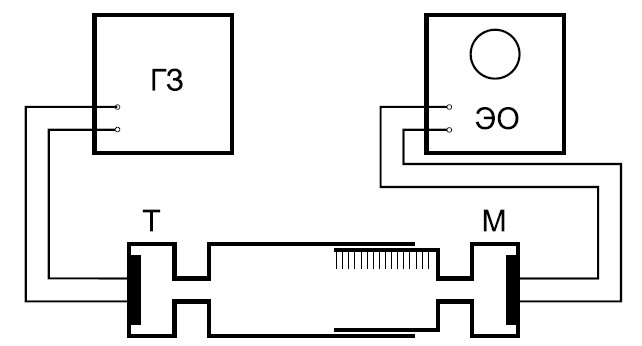
\includegraphics[width=12cm]{ust1.jpg}
		\end{center}
		\caption{Установка для измерения скорости звука при помощи раздвижной трубы}
		\label{img1}
	\end{figure}
	
	\begin{figure}[H]
		\begin{center}
			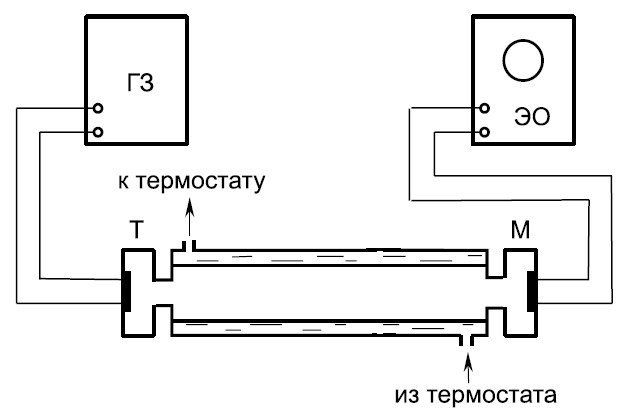
\includegraphics[width=12cm]{ust2.jpg}
		\end{center}
		\caption{Установка для изучения зависимости скорости звука от температуры}
		\label{img2}
	\end{figure}
	
	\section{Ход работы}
	
	\subsection{Измерение $ C_P/C_V $ для воздуха при помощи установки с раздвижной трубой}
	
	\label{ident}
	
	Проведём измерение коэффициента $ C_p/C_v $ для воздуха при помощи установки с раздвижной трубой. Для проведения серии измерений фиксируем частоту звукового сигнала и оставляем её неизменной при до окончания снятия показаний. Увеличиваем и уменьшаем длину трубки, чтобы добиться резонанса, возникновение которого устанавливается при помощи осциллографа. При возникновении резонанса фиксируем то расстояние, на которое была выдвинута трубка прибора. Данные измерения проводим для нескольких значений частот. Полученные результаты заносим в таблицу.
	
	\begin{table}[H]
		\centering
		\begin{tabular}{|c|c|c|c|c|c|}
		\hline
		$L$, см & $f_1$, Гц & $f_2$, Гц & $f_3$, Гц & $f_4$, Гц & $f_5$, Гц \\ \hline
		4       & 245       & 485       & 744       & 976       & 1204      \\ \hline
		5       & 235       & 480       & 731       & 958       & 1170      \\ \hline
		6       & 218       & 431       & 648       & 866       & 1096      \\ \hline
		7       & 210       & 410       & 633       & 828       & 1067      \\ \hline
		8       & 184       & 369       & 537       & 724       & 908       \\ \hline
		\end{tabular}
		\end{table}
	Для каждого измерения величины <<выдвига>> трубы $ \sigma_l = 0,5 $ мм. Также для каждого измерения вычислим $ \Delta L = L - l_0 $. Погрешность определения этой величины составит $ \sigma_{\Delta L}=~\sqrt{2}\sigma_l \approx~0,7 $~мм.
	
	По полученным данным построим графики зависимости $ f(n) $.
	
	\begin{figure}[h!]
		\centering
		%% Creator: Matplotlib, PGF backend
%%
%% To include the figure in your LaTeX document, write
%%   \input{<filename>.pgf}
%%
%% Make sure the required packages are loaded in your preamble
%%   \usepackage{pgf}
%%
%% Also ensure that all the required font packages are loaded; for instance,
%% the lmodern package is sometimes necessary when using math font.
%%   \usepackage{lmodern}
%%
%% Figures using additional raster images can only be included by \input if
%% they are in the same directory as the main LaTeX file. For loading figures
%% from other directories you can use the `import` package
%%   \usepackage{import}
%%
%% and then include the figures with
%%   \import{<path to file>}{<filename>.pgf}
%%
%% Matplotlib used the following preamble
%%   
%%   \makeatletter\@ifpackageloaded{underscore}{}{\usepackage[strings]{underscore}}\makeatother
%%
\begingroup%
\makeatletter%
\begin{pgfpicture}%
\pgfpathrectangle{\pgfpointorigin}{\pgfqpoint{7.000000in}{4.000000in}}%
\pgfusepath{use as bounding box, clip}%
\begin{pgfscope}%
\pgfsetbuttcap%
\pgfsetmiterjoin%
\definecolor{currentfill}{rgb}{1.000000,1.000000,1.000000}%
\pgfsetfillcolor{currentfill}%
\pgfsetlinewidth{0.000000pt}%
\definecolor{currentstroke}{rgb}{1.000000,1.000000,1.000000}%
\pgfsetstrokecolor{currentstroke}%
\pgfsetdash{}{0pt}%
\pgfpathmoveto{\pgfqpoint{0.000000in}{0.000000in}}%
\pgfpathlineto{\pgfqpoint{7.000000in}{0.000000in}}%
\pgfpathlineto{\pgfqpoint{7.000000in}{4.000000in}}%
\pgfpathlineto{\pgfqpoint{0.000000in}{4.000000in}}%
\pgfpathlineto{\pgfqpoint{0.000000in}{0.000000in}}%
\pgfpathclose%
\pgfusepath{fill}%
\end{pgfscope}%
\begin{pgfscope}%
\pgfsetbuttcap%
\pgfsetmiterjoin%
\definecolor{currentfill}{rgb}{1.000000,1.000000,1.000000}%
\pgfsetfillcolor{currentfill}%
\pgfsetlinewidth{0.000000pt}%
\definecolor{currentstroke}{rgb}{0.000000,0.000000,0.000000}%
\pgfsetstrokecolor{currentstroke}%
\pgfsetstrokeopacity{0.000000}%
\pgfsetdash{}{0pt}%
\pgfpathmoveto{\pgfqpoint{0.875000in}{0.440000in}}%
\pgfpathlineto{\pgfqpoint{6.300000in}{0.440000in}}%
\pgfpathlineto{\pgfqpoint{6.300000in}{3.520000in}}%
\pgfpathlineto{\pgfqpoint{0.875000in}{3.520000in}}%
\pgfpathlineto{\pgfqpoint{0.875000in}{0.440000in}}%
\pgfpathclose%
\pgfusepath{fill}%
\end{pgfscope}%
\begin{pgfscope}%
\pgfpathrectangle{\pgfqpoint{0.875000in}{0.440000in}}{\pgfqpoint{5.425000in}{3.080000in}}%
\pgfusepath{clip}%
\pgfsetbuttcap%
\pgfsetroundjoin%
\definecolor{currentfill}{rgb}{0.121569,0.466667,0.705882}%
\pgfsetfillcolor{currentfill}%
\pgfsetlinewidth{1.003750pt}%
\definecolor{currentstroke}{rgb}{0.121569,0.466667,0.705882}%
\pgfsetstrokecolor{currentstroke}%
\pgfsetdash{}{0pt}%
\pgfsys@defobject{currentmarker}{\pgfqpoint{-0.015528in}{-0.015528in}}{\pgfqpoint{0.015528in}{0.015528in}}{%
\pgfpathmoveto{\pgfqpoint{0.000000in}{-0.015528in}}%
\pgfpathcurveto{\pgfqpoint{0.004118in}{-0.015528in}}{\pgfqpoint{0.008068in}{-0.013892in}}{\pgfqpoint{0.010980in}{-0.010980in}}%
\pgfpathcurveto{\pgfqpoint{0.013892in}{-0.008068in}}{\pgfqpoint{0.015528in}{-0.004118in}}{\pgfqpoint{0.015528in}{0.000000in}}%
\pgfpathcurveto{\pgfqpoint{0.015528in}{0.004118in}}{\pgfqpoint{0.013892in}{0.008068in}}{\pgfqpoint{0.010980in}{0.010980in}}%
\pgfpathcurveto{\pgfqpoint{0.008068in}{0.013892in}}{\pgfqpoint{0.004118in}{0.015528in}}{\pgfqpoint{0.000000in}{0.015528in}}%
\pgfpathcurveto{\pgfqpoint{-0.004118in}{0.015528in}}{\pgfqpoint{-0.008068in}{0.013892in}}{\pgfqpoint{-0.010980in}{0.010980in}}%
\pgfpathcurveto{\pgfqpoint{-0.013892in}{0.008068in}}{\pgfqpoint{-0.015528in}{0.004118in}}{\pgfqpoint{-0.015528in}{0.000000in}}%
\pgfpathcurveto{\pgfqpoint{-0.015528in}{-0.004118in}}{\pgfqpoint{-0.013892in}{-0.008068in}}{\pgfqpoint{-0.010980in}{-0.010980in}}%
\pgfpathcurveto{\pgfqpoint{-0.008068in}{-0.013892in}}{\pgfqpoint{-0.004118in}{-0.015528in}}{\pgfqpoint{0.000000in}{-0.015528in}}%
\pgfpathlineto{\pgfqpoint{0.000000in}{-0.015528in}}%
\pgfpathclose%
\pgfusepath{stroke,fill}%
}%
\begin{pgfscope}%
\pgfsys@transformshift{2.107955in}{1.154347in}%
\pgfsys@useobject{currentmarker}{}%
\end{pgfscope}%
\begin{pgfscope}%
\pgfsys@transformshift{3.094318in}{1.728694in}%
\pgfsys@useobject{currentmarker}{}%
\end{pgfscope}%
\begin{pgfscope}%
\pgfsys@transformshift{4.080682in}{2.317106in}%
\pgfsys@useobject{currentmarker}{}%
\end{pgfscope}%
\begin{pgfscope}%
\pgfsys@transformshift{5.067045in}{2.849257in}%
\pgfsys@useobject{currentmarker}{}%
\end{pgfscope}%
\begin{pgfscope}%
\pgfsys@transformshift{6.053409in}{3.346242in}%
\pgfsys@useobject{currentmarker}{}%
\end{pgfscope}%
\end{pgfscope}%
\begin{pgfscope}%
\pgfpathrectangle{\pgfqpoint{0.875000in}{0.440000in}}{\pgfqpoint{5.425000in}{3.080000in}}%
\pgfusepath{clip}%
\pgfsetbuttcap%
\pgfsetroundjoin%
\definecolor{currentfill}{rgb}{1.000000,0.498039,0.054902}%
\pgfsetfillcolor{currentfill}%
\pgfsetlinewidth{1.003750pt}%
\definecolor{currentstroke}{rgb}{1.000000,0.498039,0.054902}%
\pgfsetstrokecolor{currentstroke}%
\pgfsetdash{}{0pt}%
\pgfsys@defobject{currentmarker}{\pgfqpoint{-0.015528in}{-0.015528in}}{\pgfqpoint{0.015528in}{0.015528in}}{%
\pgfpathmoveto{\pgfqpoint{0.000000in}{-0.015528in}}%
\pgfpathcurveto{\pgfqpoint{0.004118in}{-0.015528in}}{\pgfqpoint{0.008068in}{-0.013892in}}{\pgfqpoint{0.010980in}{-0.010980in}}%
\pgfpathcurveto{\pgfqpoint{0.013892in}{-0.008068in}}{\pgfqpoint{0.015528in}{-0.004118in}}{\pgfqpoint{0.015528in}{0.000000in}}%
\pgfpathcurveto{\pgfqpoint{0.015528in}{0.004118in}}{\pgfqpoint{0.013892in}{0.008068in}}{\pgfqpoint{0.010980in}{0.010980in}}%
\pgfpathcurveto{\pgfqpoint{0.008068in}{0.013892in}}{\pgfqpoint{0.004118in}{0.015528in}}{\pgfqpoint{0.000000in}{0.015528in}}%
\pgfpathcurveto{\pgfqpoint{-0.004118in}{0.015528in}}{\pgfqpoint{-0.008068in}{0.013892in}}{\pgfqpoint{-0.010980in}{0.010980in}}%
\pgfpathcurveto{\pgfqpoint{-0.013892in}{0.008068in}}{\pgfqpoint{-0.015528in}{0.004118in}}{\pgfqpoint{-0.015528in}{0.000000in}}%
\pgfpathcurveto{\pgfqpoint{-0.015528in}{-0.004118in}}{\pgfqpoint{-0.013892in}{-0.008068in}}{\pgfqpoint{-0.010980in}{-0.010980in}}%
\pgfpathcurveto{\pgfqpoint{-0.008068in}{-0.013892in}}{\pgfqpoint{-0.004118in}{-0.015528in}}{\pgfqpoint{0.000000in}{-0.015528in}}%
\pgfpathlineto{\pgfqpoint{0.000000in}{-0.015528in}}%
\pgfpathclose%
\pgfusepath{stroke,fill}%
}%
\begin{pgfscope}%
\pgfsys@transformshift{2.107955in}{1.114494in}%
\pgfsys@useobject{currentmarker}{}%
\end{pgfscope}%
\begin{pgfscope}%
\pgfsys@transformshift{3.094318in}{1.613825in}%
\pgfsys@useobject{currentmarker}{}%
\end{pgfscope}%
\begin{pgfscope}%
\pgfsys@transformshift{4.080682in}{2.122532in}%
\pgfsys@useobject{currentmarker}{}%
\end{pgfscope}%
\begin{pgfscope}%
\pgfsys@transformshift{5.067045in}{2.633583in}%
\pgfsys@useobject{currentmarker}{}%
\end{pgfscope}%
\begin{pgfscope}%
\pgfsys@transformshift{6.053409in}{3.172766in}%
\pgfsys@useobject{currentmarker}{}%
\end{pgfscope}%
\end{pgfscope}%
\begin{pgfscope}%
\pgfpathrectangle{\pgfqpoint{0.875000in}{0.440000in}}{\pgfqpoint{5.425000in}{3.080000in}}%
\pgfusepath{clip}%
\pgfsetbuttcap%
\pgfsetroundjoin%
\definecolor{currentfill}{rgb}{0.172549,0.627451,0.172549}%
\pgfsetfillcolor{currentfill}%
\pgfsetlinewidth{1.003750pt}%
\definecolor{currentstroke}{rgb}{0.172549,0.627451,0.172549}%
\pgfsetstrokecolor{currentstroke}%
\pgfsetdash{}{0pt}%
\pgfsys@defobject{currentmarker}{\pgfqpoint{-0.015528in}{-0.015528in}}{\pgfqpoint{0.015528in}{0.015528in}}{%
\pgfpathmoveto{\pgfqpoint{0.000000in}{-0.015528in}}%
\pgfpathcurveto{\pgfqpoint{0.004118in}{-0.015528in}}{\pgfqpoint{0.008068in}{-0.013892in}}{\pgfqpoint{0.010980in}{-0.010980in}}%
\pgfpathcurveto{\pgfqpoint{0.013892in}{-0.008068in}}{\pgfqpoint{0.015528in}{-0.004118in}}{\pgfqpoint{0.015528in}{0.000000in}}%
\pgfpathcurveto{\pgfqpoint{0.015528in}{0.004118in}}{\pgfqpoint{0.013892in}{0.008068in}}{\pgfqpoint{0.010980in}{0.010980in}}%
\pgfpathcurveto{\pgfqpoint{0.008068in}{0.013892in}}{\pgfqpoint{0.004118in}{0.015528in}}{\pgfqpoint{0.000000in}{0.015528in}}%
\pgfpathcurveto{\pgfqpoint{-0.004118in}{0.015528in}}{\pgfqpoint{-0.008068in}{0.013892in}}{\pgfqpoint{-0.010980in}{0.010980in}}%
\pgfpathcurveto{\pgfqpoint{-0.013892in}{0.008068in}}{\pgfqpoint{-0.015528in}{0.004118in}}{\pgfqpoint{-0.015528in}{0.000000in}}%
\pgfpathcurveto{\pgfqpoint{-0.015528in}{-0.004118in}}{\pgfqpoint{-0.013892in}{-0.008068in}}{\pgfqpoint{-0.010980in}{-0.010980in}}%
\pgfpathcurveto{\pgfqpoint{-0.008068in}{-0.013892in}}{\pgfqpoint{-0.004118in}{-0.015528in}}{\pgfqpoint{0.000000in}{-0.015528in}}%
\pgfpathlineto{\pgfqpoint{0.000000in}{-0.015528in}}%
\pgfpathclose%
\pgfusepath{stroke,fill}%
}%
\begin{pgfscope}%
\pgfsys@transformshift{2.107955in}{1.095740in}%
\pgfsys@useobject{currentmarker}{}%
\end{pgfscope}%
\begin{pgfscope}%
\pgfsys@transformshift{3.094318in}{1.564595in}%
\pgfsys@useobject{currentmarker}{}%
\end{pgfscope}%
\begin{pgfscope}%
\pgfsys@transformshift{4.080682in}{2.087368in}%
\pgfsys@useobject{currentmarker}{}%
\end{pgfscope}%
\begin{pgfscope}%
\pgfsys@transformshift{5.067045in}{2.544501in}%
\pgfsys@useobject{currentmarker}{}%
\end{pgfscope}%
\begin{pgfscope}%
\pgfsys@transformshift{6.053409in}{3.104782in}%
\pgfsys@useobject{currentmarker}{}%
\end{pgfscope}%
\end{pgfscope}%
\begin{pgfscope}%
\pgfpathrectangle{\pgfqpoint{0.875000in}{0.440000in}}{\pgfqpoint{5.425000in}{3.080000in}}%
\pgfusepath{clip}%
\pgfsetbuttcap%
\pgfsetroundjoin%
\definecolor{currentfill}{rgb}{0.839216,0.152941,0.156863}%
\pgfsetfillcolor{currentfill}%
\pgfsetlinewidth{1.003750pt}%
\definecolor{currentstroke}{rgb}{0.839216,0.152941,0.156863}%
\pgfsetstrokecolor{currentstroke}%
\pgfsetdash{}{0pt}%
\pgfsys@defobject{currentmarker}{\pgfqpoint{-0.015528in}{-0.015528in}}{\pgfqpoint{0.015528in}{0.015528in}}{%
\pgfpathmoveto{\pgfqpoint{0.000000in}{-0.015528in}}%
\pgfpathcurveto{\pgfqpoint{0.004118in}{-0.015528in}}{\pgfqpoint{0.008068in}{-0.013892in}}{\pgfqpoint{0.010980in}{-0.010980in}}%
\pgfpathcurveto{\pgfqpoint{0.013892in}{-0.008068in}}{\pgfqpoint{0.015528in}{-0.004118in}}{\pgfqpoint{0.015528in}{0.000000in}}%
\pgfpathcurveto{\pgfqpoint{0.015528in}{0.004118in}}{\pgfqpoint{0.013892in}{0.008068in}}{\pgfqpoint{0.010980in}{0.010980in}}%
\pgfpathcurveto{\pgfqpoint{0.008068in}{0.013892in}}{\pgfqpoint{0.004118in}{0.015528in}}{\pgfqpoint{0.000000in}{0.015528in}}%
\pgfpathcurveto{\pgfqpoint{-0.004118in}{0.015528in}}{\pgfqpoint{-0.008068in}{0.013892in}}{\pgfqpoint{-0.010980in}{0.010980in}}%
\pgfpathcurveto{\pgfqpoint{-0.013892in}{0.008068in}}{\pgfqpoint{-0.015528in}{0.004118in}}{\pgfqpoint{-0.015528in}{0.000000in}}%
\pgfpathcurveto{\pgfqpoint{-0.015528in}{-0.004118in}}{\pgfqpoint{-0.013892in}{-0.008068in}}{\pgfqpoint{-0.010980in}{-0.010980in}}%
\pgfpathcurveto{\pgfqpoint{-0.008068in}{-0.013892in}}{\pgfqpoint{-0.004118in}{-0.015528in}}{\pgfqpoint{0.000000in}{-0.015528in}}%
\pgfpathlineto{\pgfqpoint{0.000000in}{-0.015528in}}%
\pgfpathclose%
\pgfusepath{stroke,fill}%
}%
\begin{pgfscope}%
\pgfsys@transformshift{2.107955in}{1.034789in}%
\pgfsys@useobject{currentmarker}{}%
\end{pgfscope}%
\begin{pgfscope}%
\pgfsys@transformshift{3.094318in}{1.468480in}%
\pgfsys@useobject{currentmarker}{}%
\end{pgfscope}%
\begin{pgfscope}%
\pgfsys@transformshift{4.080682in}{1.862317in}%
\pgfsys@useobject{currentmarker}{}%
\end{pgfscope}%
\begin{pgfscope}%
\pgfsys@transformshift{5.067045in}{2.300697in}%
\pgfsys@useobject{currentmarker}{}%
\end{pgfscope}%
\begin{pgfscope}%
\pgfsys@transformshift{6.053409in}{2.732043in}%
\pgfsys@useobject{currentmarker}{}%
\end{pgfscope}%
\end{pgfscope}%
\begin{pgfscope}%
\pgfpathrectangle{\pgfqpoint{0.875000in}{0.440000in}}{\pgfqpoint{5.425000in}{3.080000in}}%
\pgfusepath{clip}%
\pgfsetrectcap%
\pgfsetroundjoin%
\pgfsetlinewidth{0.803000pt}%
\definecolor{currentstroke}{rgb}{0.690196,0.690196,0.690196}%
\pgfsetstrokecolor{currentstroke}%
\pgfsetdash{}{0pt}%
\pgfpathmoveto{\pgfqpoint{1.121591in}{0.440000in}}%
\pgfpathlineto{\pgfqpoint{1.121591in}{3.520000in}}%
\pgfusepath{stroke}%
\end{pgfscope}%
\begin{pgfscope}%
\pgfsetbuttcap%
\pgfsetroundjoin%
\definecolor{currentfill}{rgb}{0.000000,0.000000,0.000000}%
\pgfsetfillcolor{currentfill}%
\pgfsetlinewidth{0.803000pt}%
\definecolor{currentstroke}{rgb}{0.000000,0.000000,0.000000}%
\pgfsetstrokecolor{currentstroke}%
\pgfsetdash{}{0pt}%
\pgfsys@defobject{currentmarker}{\pgfqpoint{0.000000in}{-0.048611in}}{\pgfqpoint{0.000000in}{0.000000in}}{%
\pgfpathmoveto{\pgfqpoint{0.000000in}{0.000000in}}%
\pgfpathlineto{\pgfqpoint{0.000000in}{-0.048611in}}%
\pgfusepath{stroke,fill}%
}%
\begin{pgfscope}%
\pgfsys@transformshift{1.121591in}{0.440000in}%
\pgfsys@useobject{currentmarker}{}%
\end{pgfscope}%
\end{pgfscope}%
\begin{pgfscope}%
\definecolor{textcolor}{rgb}{0.000000,0.000000,0.000000}%
\pgfsetstrokecolor{textcolor}%
\pgfsetfillcolor{textcolor}%
\pgftext[x=1.121591in,y=0.342778in,,top]{\color{textcolor}\rmfamily\fontsize{10.000000}{12.000000}\selectfont \(\displaystyle {0}\)}%
\end{pgfscope}%
\begin{pgfscope}%
\pgfpathrectangle{\pgfqpoint{0.875000in}{0.440000in}}{\pgfqpoint{5.425000in}{3.080000in}}%
\pgfusepath{clip}%
\pgfsetrectcap%
\pgfsetroundjoin%
\pgfsetlinewidth{0.803000pt}%
\definecolor{currentstroke}{rgb}{0.690196,0.690196,0.690196}%
\pgfsetstrokecolor{currentstroke}%
\pgfsetdash{}{0pt}%
\pgfpathmoveto{\pgfqpoint{2.107955in}{0.440000in}}%
\pgfpathlineto{\pgfqpoint{2.107955in}{3.520000in}}%
\pgfusepath{stroke}%
\end{pgfscope}%
\begin{pgfscope}%
\pgfsetbuttcap%
\pgfsetroundjoin%
\definecolor{currentfill}{rgb}{0.000000,0.000000,0.000000}%
\pgfsetfillcolor{currentfill}%
\pgfsetlinewidth{0.803000pt}%
\definecolor{currentstroke}{rgb}{0.000000,0.000000,0.000000}%
\pgfsetstrokecolor{currentstroke}%
\pgfsetdash{}{0pt}%
\pgfsys@defobject{currentmarker}{\pgfqpoint{0.000000in}{-0.048611in}}{\pgfqpoint{0.000000in}{0.000000in}}{%
\pgfpathmoveto{\pgfqpoint{0.000000in}{0.000000in}}%
\pgfpathlineto{\pgfqpoint{0.000000in}{-0.048611in}}%
\pgfusepath{stroke,fill}%
}%
\begin{pgfscope}%
\pgfsys@transformshift{2.107955in}{0.440000in}%
\pgfsys@useobject{currentmarker}{}%
\end{pgfscope}%
\end{pgfscope}%
\begin{pgfscope}%
\definecolor{textcolor}{rgb}{0.000000,0.000000,0.000000}%
\pgfsetstrokecolor{textcolor}%
\pgfsetfillcolor{textcolor}%
\pgftext[x=2.107955in,y=0.342778in,,top]{\color{textcolor}\rmfamily\fontsize{10.000000}{12.000000}\selectfont \(\displaystyle {1}\)}%
\end{pgfscope}%
\begin{pgfscope}%
\pgfpathrectangle{\pgfqpoint{0.875000in}{0.440000in}}{\pgfqpoint{5.425000in}{3.080000in}}%
\pgfusepath{clip}%
\pgfsetrectcap%
\pgfsetroundjoin%
\pgfsetlinewidth{0.803000pt}%
\definecolor{currentstroke}{rgb}{0.690196,0.690196,0.690196}%
\pgfsetstrokecolor{currentstroke}%
\pgfsetdash{}{0pt}%
\pgfpathmoveto{\pgfqpoint{3.094318in}{0.440000in}}%
\pgfpathlineto{\pgfqpoint{3.094318in}{3.520000in}}%
\pgfusepath{stroke}%
\end{pgfscope}%
\begin{pgfscope}%
\pgfsetbuttcap%
\pgfsetroundjoin%
\definecolor{currentfill}{rgb}{0.000000,0.000000,0.000000}%
\pgfsetfillcolor{currentfill}%
\pgfsetlinewidth{0.803000pt}%
\definecolor{currentstroke}{rgb}{0.000000,0.000000,0.000000}%
\pgfsetstrokecolor{currentstroke}%
\pgfsetdash{}{0pt}%
\pgfsys@defobject{currentmarker}{\pgfqpoint{0.000000in}{-0.048611in}}{\pgfqpoint{0.000000in}{0.000000in}}{%
\pgfpathmoveto{\pgfqpoint{0.000000in}{0.000000in}}%
\pgfpathlineto{\pgfqpoint{0.000000in}{-0.048611in}}%
\pgfusepath{stroke,fill}%
}%
\begin{pgfscope}%
\pgfsys@transformshift{3.094318in}{0.440000in}%
\pgfsys@useobject{currentmarker}{}%
\end{pgfscope}%
\end{pgfscope}%
\begin{pgfscope}%
\definecolor{textcolor}{rgb}{0.000000,0.000000,0.000000}%
\pgfsetstrokecolor{textcolor}%
\pgfsetfillcolor{textcolor}%
\pgftext[x=3.094318in,y=0.342778in,,top]{\color{textcolor}\rmfamily\fontsize{10.000000}{12.000000}\selectfont \(\displaystyle {2}\)}%
\end{pgfscope}%
\begin{pgfscope}%
\pgfpathrectangle{\pgfqpoint{0.875000in}{0.440000in}}{\pgfqpoint{5.425000in}{3.080000in}}%
\pgfusepath{clip}%
\pgfsetrectcap%
\pgfsetroundjoin%
\pgfsetlinewidth{0.803000pt}%
\definecolor{currentstroke}{rgb}{0.690196,0.690196,0.690196}%
\pgfsetstrokecolor{currentstroke}%
\pgfsetdash{}{0pt}%
\pgfpathmoveto{\pgfqpoint{4.080682in}{0.440000in}}%
\pgfpathlineto{\pgfqpoint{4.080682in}{3.520000in}}%
\pgfusepath{stroke}%
\end{pgfscope}%
\begin{pgfscope}%
\pgfsetbuttcap%
\pgfsetroundjoin%
\definecolor{currentfill}{rgb}{0.000000,0.000000,0.000000}%
\pgfsetfillcolor{currentfill}%
\pgfsetlinewidth{0.803000pt}%
\definecolor{currentstroke}{rgb}{0.000000,0.000000,0.000000}%
\pgfsetstrokecolor{currentstroke}%
\pgfsetdash{}{0pt}%
\pgfsys@defobject{currentmarker}{\pgfqpoint{0.000000in}{-0.048611in}}{\pgfqpoint{0.000000in}{0.000000in}}{%
\pgfpathmoveto{\pgfqpoint{0.000000in}{0.000000in}}%
\pgfpathlineto{\pgfqpoint{0.000000in}{-0.048611in}}%
\pgfusepath{stroke,fill}%
}%
\begin{pgfscope}%
\pgfsys@transformshift{4.080682in}{0.440000in}%
\pgfsys@useobject{currentmarker}{}%
\end{pgfscope}%
\end{pgfscope}%
\begin{pgfscope}%
\definecolor{textcolor}{rgb}{0.000000,0.000000,0.000000}%
\pgfsetstrokecolor{textcolor}%
\pgfsetfillcolor{textcolor}%
\pgftext[x=4.080682in,y=0.342778in,,top]{\color{textcolor}\rmfamily\fontsize{10.000000}{12.000000}\selectfont \(\displaystyle {3}\)}%
\end{pgfscope}%
\begin{pgfscope}%
\pgfpathrectangle{\pgfqpoint{0.875000in}{0.440000in}}{\pgfqpoint{5.425000in}{3.080000in}}%
\pgfusepath{clip}%
\pgfsetrectcap%
\pgfsetroundjoin%
\pgfsetlinewidth{0.803000pt}%
\definecolor{currentstroke}{rgb}{0.690196,0.690196,0.690196}%
\pgfsetstrokecolor{currentstroke}%
\pgfsetdash{}{0pt}%
\pgfpathmoveto{\pgfqpoint{5.067045in}{0.440000in}}%
\pgfpathlineto{\pgfqpoint{5.067045in}{3.520000in}}%
\pgfusepath{stroke}%
\end{pgfscope}%
\begin{pgfscope}%
\pgfsetbuttcap%
\pgfsetroundjoin%
\definecolor{currentfill}{rgb}{0.000000,0.000000,0.000000}%
\pgfsetfillcolor{currentfill}%
\pgfsetlinewidth{0.803000pt}%
\definecolor{currentstroke}{rgb}{0.000000,0.000000,0.000000}%
\pgfsetstrokecolor{currentstroke}%
\pgfsetdash{}{0pt}%
\pgfsys@defobject{currentmarker}{\pgfqpoint{0.000000in}{-0.048611in}}{\pgfqpoint{0.000000in}{0.000000in}}{%
\pgfpathmoveto{\pgfqpoint{0.000000in}{0.000000in}}%
\pgfpathlineto{\pgfqpoint{0.000000in}{-0.048611in}}%
\pgfusepath{stroke,fill}%
}%
\begin{pgfscope}%
\pgfsys@transformshift{5.067045in}{0.440000in}%
\pgfsys@useobject{currentmarker}{}%
\end{pgfscope}%
\end{pgfscope}%
\begin{pgfscope}%
\definecolor{textcolor}{rgb}{0.000000,0.000000,0.000000}%
\pgfsetstrokecolor{textcolor}%
\pgfsetfillcolor{textcolor}%
\pgftext[x=5.067045in,y=0.342778in,,top]{\color{textcolor}\rmfamily\fontsize{10.000000}{12.000000}\selectfont \(\displaystyle {4}\)}%
\end{pgfscope}%
\begin{pgfscope}%
\pgfpathrectangle{\pgfqpoint{0.875000in}{0.440000in}}{\pgfqpoint{5.425000in}{3.080000in}}%
\pgfusepath{clip}%
\pgfsetrectcap%
\pgfsetroundjoin%
\pgfsetlinewidth{0.803000pt}%
\definecolor{currentstroke}{rgb}{0.690196,0.690196,0.690196}%
\pgfsetstrokecolor{currentstroke}%
\pgfsetdash{}{0pt}%
\pgfpathmoveto{\pgfqpoint{6.053409in}{0.440000in}}%
\pgfpathlineto{\pgfqpoint{6.053409in}{3.520000in}}%
\pgfusepath{stroke}%
\end{pgfscope}%
\begin{pgfscope}%
\pgfsetbuttcap%
\pgfsetroundjoin%
\definecolor{currentfill}{rgb}{0.000000,0.000000,0.000000}%
\pgfsetfillcolor{currentfill}%
\pgfsetlinewidth{0.803000pt}%
\definecolor{currentstroke}{rgb}{0.000000,0.000000,0.000000}%
\pgfsetstrokecolor{currentstroke}%
\pgfsetdash{}{0pt}%
\pgfsys@defobject{currentmarker}{\pgfqpoint{0.000000in}{-0.048611in}}{\pgfqpoint{0.000000in}{0.000000in}}{%
\pgfpathmoveto{\pgfqpoint{0.000000in}{0.000000in}}%
\pgfpathlineto{\pgfqpoint{0.000000in}{-0.048611in}}%
\pgfusepath{stroke,fill}%
}%
\begin{pgfscope}%
\pgfsys@transformshift{6.053409in}{0.440000in}%
\pgfsys@useobject{currentmarker}{}%
\end{pgfscope}%
\end{pgfscope}%
\begin{pgfscope}%
\definecolor{textcolor}{rgb}{0.000000,0.000000,0.000000}%
\pgfsetstrokecolor{textcolor}%
\pgfsetfillcolor{textcolor}%
\pgftext[x=6.053409in,y=0.342778in,,top]{\color{textcolor}\rmfamily\fontsize{10.000000}{12.000000}\selectfont \(\displaystyle {5}\)}%
\end{pgfscope}%
\begin{pgfscope}%
\definecolor{textcolor}{rgb}{0.000000,0.000000,0.000000}%
\pgfsetstrokecolor{textcolor}%
\pgfsetfillcolor{textcolor}%
\pgftext[x=3.587500in,y=0.163766in,,top]{\color{textcolor}\rmfamily\fontsize{10.000000}{12.000000}\selectfont \(\displaystyle n\)}%
\end{pgfscope}%
\begin{pgfscope}%
\pgfpathrectangle{\pgfqpoint{0.875000in}{0.440000in}}{\pgfqpoint{5.425000in}{3.080000in}}%
\pgfusepath{clip}%
\pgfsetrectcap%
\pgfsetroundjoin%
\pgfsetlinewidth{0.803000pt}%
\definecolor{currentstroke}{rgb}{0.690196,0.690196,0.690196}%
\pgfsetstrokecolor{currentstroke}%
\pgfsetdash{}{0pt}%
\pgfpathmoveto{\pgfqpoint{0.875000in}{0.603443in}}%
\pgfpathlineto{\pgfqpoint{6.300000in}{0.603443in}}%
\pgfusepath{stroke}%
\end{pgfscope}%
\begin{pgfscope}%
\pgfsetbuttcap%
\pgfsetroundjoin%
\definecolor{currentfill}{rgb}{0.000000,0.000000,0.000000}%
\pgfsetfillcolor{currentfill}%
\pgfsetlinewidth{0.803000pt}%
\definecolor{currentstroke}{rgb}{0.000000,0.000000,0.000000}%
\pgfsetstrokecolor{currentstroke}%
\pgfsetdash{}{0pt}%
\pgfsys@defobject{currentmarker}{\pgfqpoint{-0.048611in}{0.000000in}}{\pgfqpoint{-0.000000in}{0.000000in}}{%
\pgfpathmoveto{\pgfqpoint{-0.000000in}{0.000000in}}%
\pgfpathlineto{\pgfqpoint{-0.048611in}{0.000000in}}%
\pgfusepath{stroke,fill}%
}%
\begin{pgfscope}%
\pgfsys@transformshift{0.875000in}{0.603443in}%
\pgfsys@useobject{currentmarker}{}%
\end{pgfscope}%
\end{pgfscope}%
\begin{pgfscope}%
\definecolor{textcolor}{rgb}{0.000000,0.000000,0.000000}%
\pgfsetstrokecolor{textcolor}%
\pgfsetfillcolor{textcolor}%
\pgftext[x=0.708333in, y=0.555217in, left, base]{\color{textcolor}\rmfamily\fontsize{10.000000}{12.000000}\selectfont \(\displaystyle {0}\)}%
\end{pgfscope}%
\begin{pgfscope}%
\pgfpathrectangle{\pgfqpoint{0.875000in}{0.440000in}}{\pgfqpoint{5.425000in}{3.080000in}}%
\pgfusepath{clip}%
\pgfsetrectcap%
\pgfsetroundjoin%
\pgfsetlinewidth{0.803000pt}%
\definecolor{currentstroke}{rgb}{0.690196,0.690196,0.690196}%
\pgfsetstrokecolor{currentstroke}%
\pgfsetdash{}{0pt}%
\pgfpathmoveto{\pgfqpoint{0.875000in}{1.072297in}}%
\pgfpathlineto{\pgfqpoint{6.300000in}{1.072297in}}%
\pgfusepath{stroke}%
\end{pgfscope}%
\begin{pgfscope}%
\pgfsetbuttcap%
\pgfsetroundjoin%
\definecolor{currentfill}{rgb}{0.000000,0.000000,0.000000}%
\pgfsetfillcolor{currentfill}%
\pgfsetlinewidth{0.803000pt}%
\definecolor{currentstroke}{rgb}{0.000000,0.000000,0.000000}%
\pgfsetstrokecolor{currentstroke}%
\pgfsetdash{}{0pt}%
\pgfsys@defobject{currentmarker}{\pgfqpoint{-0.048611in}{0.000000in}}{\pgfqpoint{-0.000000in}{0.000000in}}{%
\pgfpathmoveto{\pgfqpoint{-0.000000in}{0.000000in}}%
\pgfpathlineto{\pgfqpoint{-0.048611in}{0.000000in}}%
\pgfusepath{stroke,fill}%
}%
\begin{pgfscope}%
\pgfsys@transformshift{0.875000in}{1.072297in}%
\pgfsys@useobject{currentmarker}{}%
\end{pgfscope}%
\end{pgfscope}%
\begin{pgfscope}%
\definecolor{textcolor}{rgb}{0.000000,0.000000,0.000000}%
\pgfsetstrokecolor{textcolor}%
\pgfsetfillcolor{textcolor}%
\pgftext[x=0.569444in, y=1.024072in, left, base]{\color{textcolor}\rmfamily\fontsize{10.000000}{12.000000}\selectfont \(\displaystyle {200}\)}%
\end{pgfscope}%
\begin{pgfscope}%
\pgfpathrectangle{\pgfqpoint{0.875000in}{0.440000in}}{\pgfqpoint{5.425000in}{3.080000in}}%
\pgfusepath{clip}%
\pgfsetrectcap%
\pgfsetroundjoin%
\pgfsetlinewidth{0.803000pt}%
\definecolor{currentstroke}{rgb}{0.690196,0.690196,0.690196}%
\pgfsetstrokecolor{currentstroke}%
\pgfsetdash{}{0pt}%
\pgfpathmoveto{\pgfqpoint{0.875000in}{1.541152in}}%
\pgfpathlineto{\pgfqpoint{6.300000in}{1.541152in}}%
\pgfusepath{stroke}%
\end{pgfscope}%
\begin{pgfscope}%
\pgfsetbuttcap%
\pgfsetroundjoin%
\definecolor{currentfill}{rgb}{0.000000,0.000000,0.000000}%
\pgfsetfillcolor{currentfill}%
\pgfsetlinewidth{0.803000pt}%
\definecolor{currentstroke}{rgb}{0.000000,0.000000,0.000000}%
\pgfsetstrokecolor{currentstroke}%
\pgfsetdash{}{0pt}%
\pgfsys@defobject{currentmarker}{\pgfqpoint{-0.048611in}{0.000000in}}{\pgfqpoint{-0.000000in}{0.000000in}}{%
\pgfpathmoveto{\pgfqpoint{-0.000000in}{0.000000in}}%
\pgfpathlineto{\pgfqpoint{-0.048611in}{0.000000in}}%
\pgfusepath{stroke,fill}%
}%
\begin{pgfscope}%
\pgfsys@transformshift{0.875000in}{1.541152in}%
\pgfsys@useobject{currentmarker}{}%
\end{pgfscope}%
\end{pgfscope}%
\begin{pgfscope}%
\definecolor{textcolor}{rgb}{0.000000,0.000000,0.000000}%
\pgfsetstrokecolor{textcolor}%
\pgfsetfillcolor{textcolor}%
\pgftext[x=0.569444in, y=1.492927in, left, base]{\color{textcolor}\rmfamily\fontsize{10.000000}{12.000000}\selectfont \(\displaystyle {400}\)}%
\end{pgfscope}%
\begin{pgfscope}%
\pgfpathrectangle{\pgfqpoint{0.875000in}{0.440000in}}{\pgfqpoint{5.425000in}{3.080000in}}%
\pgfusepath{clip}%
\pgfsetrectcap%
\pgfsetroundjoin%
\pgfsetlinewidth{0.803000pt}%
\definecolor{currentstroke}{rgb}{0.690196,0.690196,0.690196}%
\pgfsetstrokecolor{currentstroke}%
\pgfsetdash{}{0pt}%
\pgfpathmoveto{\pgfqpoint{0.875000in}{2.010007in}}%
\pgfpathlineto{\pgfqpoint{6.300000in}{2.010007in}}%
\pgfusepath{stroke}%
\end{pgfscope}%
\begin{pgfscope}%
\pgfsetbuttcap%
\pgfsetroundjoin%
\definecolor{currentfill}{rgb}{0.000000,0.000000,0.000000}%
\pgfsetfillcolor{currentfill}%
\pgfsetlinewidth{0.803000pt}%
\definecolor{currentstroke}{rgb}{0.000000,0.000000,0.000000}%
\pgfsetstrokecolor{currentstroke}%
\pgfsetdash{}{0pt}%
\pgfsys@defobject{currentmarker}{\pgfqpoint{-0.048611in}{0.000000in}}{\pgfqpoint{-0.000000in}{0.000000in}}{%
\pgfpathmoveto{\pgfqpoint{-0.000000in}{0.000000in}}%
\pgfpathlineto{\pgfqpoint{-0.048611in}{0.000000in}}%
\pgfusepath{stroke,fill}%
}%
\begin{pgfscope}%
\pgfsys@transformshift{0.875000in}{2.010007in}%
\pgfsys@useobject{currentmarker}{}%
\end{pgfscope}%
\end{pgfscope}%
\begin{pgfscope}%
\definecolor{textcolor}{rgb}{0.000000,0.000000,0.000000}%
\pgfsetstrokecolor{textcolor}%
\pgfsetfillcolor{textcolor}%
\pgftext[x=0.569444in, y=1.961781in, left, base]{\color{textcolor}\rmfamily\fontsize{10.000000}{12.000000}\selectfont \(\displaystyle {600}\)}%
\end{pgfscope}%
\begin{pgfscope}%
\pgfpathrectangle{\pgfqpoint{0.875000in}{0.440000in}}{\pgfqpoint{5.425000in}{3.080000in}}%
\pgfusepath{clip}%
\pgfsetrectcap%
\pgfsetroundjoin%
\pgfsetlinewidth{0.803000pt}%
\definecolor{currentstroke}{rgb}{0.690196,0.690196,0.690196}%
\pgfsetstrokecolor{currentstroke}%
\pgfsetdash{}{0pt}%
\pgfpathmoveto{\pgfqpoint{0.875000in}{2.478861in}}%
\pgfpathlineto{\pgfqpoint{6.300000in}{2.478861in}}%
\pgfusepath{stroke}%
\end{pgfscope}%
\begin{pgfscope}%
\pgfsetbuttcap%
\pgfsetroundjoin%
\definecolor{currentfill}{rgb}{0.000000,0.000000,0.000000}%
\pgfsetfillcolor{currentfill}%
\pgfsetlinewidth{0.803000pt}%
\definecolor{currentstroke}{rgb}{0.000000,0.000000,0.000000}%
\pgfsetstrokecolor{currentstroke}%
\pgfsetdash{}{0pt}%
\pgfsys@defobject{currentmarker}{\pgfqpoint{-0.048611in}{0.000000in}}{\pgfqpoint{-0.000000in}{0.000000in}}{%
\pgfpathmoveto{\pgfqpoint{-0.000000in}{0.000000in}}%
\pgfpathlineto{\pgfqpoint{-0.048611in}{0.000000in}}%
\pgfusepath{stroke,fill}%
}%
\begin{pgfscope}%
\pgfsys@transformshift{0.875000in}{2.478861in}%
\pgfsys@useobject{currentmarker}{}%
\end{pgfscope}%
\end{pgfscope}%
\begin{pgfscope}%
\definecolor{textcolor}{rgb}{0.000000,0.000000,0.000000}%
\pgfsetstrokecolor{textcolor}%
\pgfsetfillcolor{textcolor}%
\pgftext[x=0.569444in, y=2.430636in, left, base]{\color{textcolor}\rmfamily\fontsize{10.000000}{12.000000}\selectfont \(\displaystyle {800}\)}%
\end{pgfscope}%
\begin{pgfscope}%
\pgfpathrectangle{\pgfqpoint{0.875000in}{0.440000in}}{\pgfqpoint{5.425000in}{3.080000in}}%
\pgfusepath{clip}%
\pgfsetrectcap%
\pgfsetroundjoin%
\pgfsetlinewidth{0.803000pt}%
\definecolor{currentstroke}{rgb}{0.690196,0.690196,0.690196}%
\pgfsetstrokecolor{currentstroke}%
\pgfsetdash{}{0pt}%
\pgfpathmoveto{\pgfqpoint{0.875000in}{2.947716in}}%
\pgfpathlineto{\pgfqpoint{6.300000in}{2.947716in}}%
\pgfusepath{stroke}%
\end{pgfscope}%
\begin{pgfscope}%
\pgfsetbuttcap%
\pgfsetroundjoin%
\definecolor{currentfill}{rgb}{0.000000,0.000000,0.000000}%
\pgfsetfillcolor{currentfill}%
\pgfsetlinewidth{0.803000pt}%
\definecolor{currentstroke}{rgb}{0.000000,0.000000,0.000000}%
\pgfsetstrokecolor{currentstroke}%
\pgfsetdash{}{0pt}%
\pgfsys@defobject{currentmarker}{\pgfqpoint{-0.048611in}{0.000000in}}{\pgfqpoint{-0.000000in}{0.000000in}}{%
\pgfpathmoveto{\pgfqpoint{-0.000000in}{0.000000in}}%
\pgfpathlineto{\pgfqpoint{-0.048611in}{0.000000in}}%
\pgfusepath{stroke,fill}%
}%
\begin{pgfscope}%
\pgfsys@transformshift{0.875000in}{2.947716in}%
\pgfsys@useobject{currentmarker}{}%
\end{pgfscope}%
\end{pgfscope}%
\begin{pgfscope}%
\definecolor{textcolor}{rgb}{0.000000,0.000000,0.000000}%
\pgfsetstrokecolor{textcolor}%
\pgfsetfillcolor{textcolor}%
\pgftext[x=0.499999in, y=2.899491in, left, base]{\color{textcolor}\rmfamily\fontsize{10.000000}{12.000000}\selectfont \(\displaystyle {1000}\)}%
\end{pgfscope}%
\begin{pgfscope}%
\pgfpathrectangle{\pgfqpoint{0.875000in}{0.440000in}}{\pgfqpoint{5.425000in}{3.080000in}}%
\pgfusepath{clip}%
\pgfsetrectcap%
\pgfsetroundjoin%
\pgfsetlinewidth{0.803000pt}%
\definecolor{currentstroke}{rgb}{0.690196,0.690196,0.690196}%
\pgfsetstrokecolor{currentstroke}%
\pgfsetdash{}{0pt}%
\pgfpathmoveto{\pgfqpoint{0.875000in}{3.416571in}}%
\pgfpathlineto{\pgfqpoint{6.300000in}{3.416571in}}%
\pgfusepath{stroke}%
\end{pgfscope}%
\begin{pgfscope}%
\pgfsetbuttcap%
\pgfsetroundjoin%
\definecolor{currentfill}{rgb}{0.000000,0.000000,0.000000}%
\pgfsetfillcolor{currentfill}%
\pgfsetlinewidth{0.803000pt}%
\definecolor{currentstroke}{rgb}{0.000000,0.000000,0.000000}%
\pgfsetstrokecolor{currentstroke}%
\pgfsetdash{}{0pt}%
\pgfsys@defobject{currentmarker}{\pgfqpoint{-0.048611in}{0.000000in}}{\pgfqpoint{-0.000000in}{0.000000in}}{%
\pgfpathmoveto{\pgfqpoint{-0.000000in}{0.000000in}}%
\pgfpathlineto{\pgfqpoint{-0.048611in}{0.000000in}}%
\pgfusepath{stroke,fill}%
}%
\begin{pgfscope}%
\pgfsys@transformshift{0.875000in}{3.416571in}%
\pgfsys@useobject{currentmarker}{}%
\end{pgfscope}%
\end{pgfscope}%
\begin{pgfscope}%
\definecolor{textcolor}{rgb}{0.000000,0.000000,0.000000}%
\pgfsetstrokecolor{textcolor}%
\pgfsetfillcolor{textcolor}%
\pgftext[x=0.499999in, y=3.368345in, left, base]{\color{textcolor}\rmfamily\fontsize{10.000000}{12.000000}\selectfont \(\displaystyle {1200}\)}%
\end{pgfscope}%
\begin{pgfscope}%
\definecolor{textcolor}{rgb}{0.000000,0.000000,0.000000}%
\pgfsetstrokecolor{textcolor}%
\pgfsetfillcolor{textcolor}%
\pgftext[x=0.444444in,y=1.980000in,,bottom,rotate=90.000000]{\color{textcolor}\rmfamily\fontsize{10.000000}{12.000000}\selectfont \(\displaystyle f\), Hz}%
\end{pgfscope}%
\begin{pgfscope}%
\pgfpathrectangle{\pgfqpoint{0.875000in}{0.440000in}}{\pgfqpoint{5.425000in}{3.080000in}}%
\pgfusepath{clip}%
\pgfsetrectcap%
\pgfsetroundjoin%
\pgfsetlinewidth{1.505625pt}%
\definecolor{currentstroke}{rgb}{0.121569,0.466667,0.705882}%
\pgfsetstrokecolor{currentstroke}%
\pgfsetdash{}{0pt}%
\pgfpathmoveto{\pgfqpoint{1.121591in}{0.627823in}}%
\pgfpathlineto{\pgfqpoint{1.171407in}{0.655623in}}%
\pgfpathlineto{\pgfqpoint{1.221224in}{0.683423in}}%
\pgfpathlineto{\pgfqpoint{1.271040in}{0.711222in}}%
\pgfpathlineto{\pgfqpoint{1.320856in}{0.739022in}}%
\pgfpathlineto{\pgfqpoint{1.370673in}{0.766822in}}%
\pgfpathlineto{\pgfqpoint{1.420489in}{0.794622in}}%
\pgfpathlineto{\pgfqpoint{1.470305in}{0.822422in}}%
\pgfpathlineto{\pgfqpoint{1.520122in}{0.850221in}}%
\pgfpathlineto{\pgfqpoint{1.569938in}{0.878021in}}%
\pgfpathlineto{\pgfqpoint{1.619754in}{0.905821in}}%
\pgfpathlineto{\pgfqpoint{1.669571in}{0.933621in}}%
\pgfpathlineto{\pgfqpoint{1.719387in}{0.961420in}}%
\pgfpathlineto{\pgfqpoint{1.769203in}{0.989220in}}%
\pgfpathlineto{\pgfqpoint{1.819020in}{1.017020in}}%
\pgfpathlineto{\pgfqpoint{1.868836in}{1.044820in}}%
\pgfpathlineto{\pgfqpoint{1.918652in}{1.072619in}}%
\pgfpathlineto{\pgfqpoint{1.968469in}{1.100419in}}%
\pgfpathlineto{\pgfqpoint{2.018285in}{1.128219in}}%
\pgfpathlineto{\pgfqpoint{2.068101in}{1.156019in}}%
\pgfpathlineto{\pgfqpoint{2.117918in}{1.183818in}}%
\pgfpathlineto{\pgfqpoint{2.167734in}{1.211618in}}%
\pgfpathlineto{\pgfqpoint{2.217551in}{1.239418in}}%
\pgfpathlineto{\pgfqpoint{2.267367in}{1.267218in}}%
\pgfpathlineto{\pgfqpoint{2.317183in}{1.295018in}}%
\pgfpathlineto{\pgfqpoint{2.367000in}{1.322817in}}%
\pgfpathlineto{\pgfqpoint{2.416816in}{1.350617in}}%
\pgfpathlineto{\pgfqpoint{2.466632in}{1.378417in}}%
\pgfpathlineto{\pgfqpoint{2.516449in}{1.406217in}}%
\pgfpathlineto{\pgfqpoint{2.566265in}{1.434016in}}%
\pgfpathlineto{\pgfqpoint{2.616081in}{1.461816in}}%
\pgfpathlineto{\pgfqpoint{2.665898in}{1.489616in}}%
\pgfpathlineto{\pgfqpoint{2.715714in}{1.517416in}}%
\pgfpathlineto{\pgfqpoint{2.765530in}{1.545215in}}%
\pgfpathlineto{\pgfqpoint{2.815347in}{1.573015in}}%
\pgfpathlineto{\pgfqpoint{2.865163in}{1.600815in}}%
\pgfpathlineto{\pgfqpoint{2.914979in}{1.628615in}}%
\pgfpathlineto{\pgfqpoint{2.964796in}{1.656415in}}%
\pgfpathlineto{\pgfqpoint{3.014612in}{1.684214in}}%
\pgfpathlineto{\pgfqpoint{3.064428in}{1.712014in}}%
\pgfpathlineto{\pgfqpoint{3.114245in}{1.739814in}}%
\pgfpathlineto{\pgfqpoint{3.164061in}{1.767614in}}%
\pgfpathlineto{\pgfqpoint{3.213877in}{1.795413in}}%
\pgfpathlineto{\pgfqpoint{3.263694in}{1.823213in}}%
\pgfpathlineto{\pgfqpoint{3.313510in}{1.851013in}}%
\pgfpathlineto{\pgfqpoint{3.363326in}{1.878813in}}%
\pgfpathlineto{\pgfqpoint{3.413143in}{1.906612in}}%
\pgfpathlineto{\pgfqpoint{3.462959in}{1.934412in}}%
\pgfpathlineto{\pgfqpoint{3.512775in}{1.962212in}}%
\pgfpathlineto{\pgfqpoint{3.562592in}{1.990012in}}%
\pgfpathlineto{\pgfqpoint{3.612408in}{2.017811in}}%
\pgfpathlineto{\pgfqpoint{3.662225in}{2.045611in}}%
\pgfpathlineto{\pgfqpoint{3.712041in}{2.073411in}}%
\pgfpathlineto{\pgfqpoint{3.761857in}{2.101211in}}%
\pgfpathlineto{\pgfqpoint{3.811674in}{2.129011in}}%
\pgfpathlineto{\pgfqpoint{3.861490in}{2.156810in}}%
\pgfpathlineto{\pgfqpoint{3.911306in}{2.184610in}}%
\pgfpathlineto{\pgfqpoint{3.961123in}{2.212410in}}%
\pgfpathlineto{\pgfqpoint{4.010939in}{2.240210in}}%
\pgfpathlineto{\pgfqpoint{4.060755in}{2.268009in}}%
\pgfpathlineto{\pgfqpoint{4.110572in}{2.295809in}}%
\pgfpathlineto{\pgfqpoint{4.160388in}{2.323609in}}%
\pgfpathlineto{\pgfqpoint{4.210204in}{2.351409in}}%
\pgfpathlineto{\pgfqpoint{4.260021in}{2.379208in}}%
\pgfpathlineto{\pgfqpoint{4.309837in}{2.407008in}}%
\pgfpathlineto{\pgfqpoint{4.359653in}{2.434808in}}%
\pgfpathlineto{\pgfqpoint{4.409470in}{2.462608in}}%
\pgfpathlineto{\pgfqpoint{4.459286in}{2.490407in}}%
\pgfpathlineto{\pgfqpoint{4.509102in}{2.518207in}}%
\pgfpathlineto{\pgfqpoint{4.558919in}{2.546007in}}%
\pgfpathlineto{\pgfqpoint{4.608735in}{2.573807in}}%
\pgfpathlineto{\pgfqpoint{4.658551in}{2.601607in}}%
\pgfpathlineto{\pgfqpoint{4.708368in}{2.629406in}}%
\pgfpathlineto{\pgfqpoint{4.758184in}{2.657206in}}%
\pgfpathlineto{\pgfqpoint{4.808000in}{2.685006in}}%
\pgfpathlineto{\pgfqpoint{4.857817in}{2.712806in}}%
\pgfpathlineto{\pgfqpoint{4.907633in}{2.740605in}}%
\pgfpathlineto{\pgfqpoint{4.957449in}{2.768405in}}%
\pgfpathlineto{\pgfqpoint{5.007266in}{2.796205in}}%
\pgfpathlineto{\pgfqpoint{5.057082in}{2.824005in}}%
\pgfpathlineto{\pgfqpoint{5.106899in}{2.851804in}}%
\pgfpathlineto{\pgfqpoint{5.156715in}{2.879604in}}%
\pgfpathlineto{\pgfqpoint{5.206531in}{2.907404in}}%
\pgfpathlineto{\pgfqpoint{5.256348in}{2.935204in}}%
\pgfpathlineto{\pgfqpoint{5.306164in}{2.963004in}}%
\pgfpathlineto{\pgfqpoint{5.355980in}{2.990803in}}%
\pgfpathlineto{\pgfqpoint{5.405797in}{3.018603in}}%
\pgfpathlineto{\pgfqpoint{5.455613in}{3.046403in}}%
\pgfpathlineto{\pgfqpoint{5.505429in}{3.074203in}}%
\pgfpathlineto{\pgfqpoint{5.555246in}{3.102002in}}%
\pgfpathlineto{\pgfqpoint{5.605062in}{3.129802in}}%
\pgfpathlineto{\pgfqpoint{5.654878in}{3.157602in}}%
\pgfpathlineto{\pgfqpoint{5.704695in}{3.185402in}}%
\pgfpathlineto{\pgfqpoint{5.754511in}{3.213201in}}%
\pgfpathlineto{\pgfqpoint{5.804327in}{3.241001in}}%
\pgfpathlineto{\pgfqpoint{5.854144in}{3.268801in}}%
\pgfpathlineto{\pgfqpoint{5.903960in}{3.296601in}}%
\pgfpathlineto{\pgfqpoint{5.953776in}{3.324400in}}%
\pgfpathlineto{\pgfqpoint{6.003593in}{3.352200in}}%
\pgfpathlineto{\pgfqpoint{6.053409in}{3.380000in}}%
\pgfusepath{stroke}%
\end{pgfscope}%
\begin{pgfscope}%
\pgfpathrectangle{\pgfqpoint{0.875000in}{0.440000in}}{\pgfqpoint{5.425000in}{3.080000in}}%
\pgfusepath{clip}%
\pgfsetrectcap%
\pgfsetroundjoin%
\pgfsetlinewidth{1.505625pt}%
\definecolor{currentstroke}{rgb}{1.000000,0.498039,0.054902}%
\pgfsetstrokecolor{currentstroke}%
\pgfsetdash{}{0pt}%
\pgfpathmoveto{\pgfqpoint{1.121591in}{0.590549in}}%
\pgfpathlineto{\pgfqpoint{1.171407in}{0.616490in}}%
\pgfpathlineto{\pgfqpoint{1.221224in}{0.642431in}}%
\pgfpathlineto{\pgfqpoint{1.271040in}{0.668372in}}%
\pgfpathlineto{\pgfqpoint{1.320856in}{0.694313in}}%
\pgfpathlineto{\pgfqpoint{1.370673in}{0.720254in}}%
\pgfpathlineto{\pgfqpoint{1.420489in}{0.746195in}}%
\pgfpathlineto{\pgfqpoint{1.470305in}{0.772136in}}%
\pgfpathlineto{\pgfqpoint{1.520122in}{0.798077in}}%
\pgfpathlineto{\pgfqpoint{1.569938in}{0.824018in}}%
\pgfpathlineto{\pgfqpoint{1.619754in}{0.849958in}}%
\pgfpathlineto{\pgfqpoint{1.669571in}{0.875899in}}%
\pgfpathlineto{\pgfqpoint{1.719387in}{0.901840in}}%
\pgfpathlineto{\pgfqpoint{1.769203in}{0.927781in}}%
\pgfpathlineto{\pgfqpoint{1.819020in}{0.953722in}}%
\pgfpathlineto{\pgfqpoint{1.868836in}{0.979663in}}%
\pgfpathlineto{\pgfqpoint{1.918652in}{1.005604in}}%
\pgfpathlineto{\pgfqpoint{1.968469in}{1.031545in}}%
\pgfpathlineto{\pgfqpoint{2.018285in}{1.057486in}}%
\pgfpathlineto{\pgfqpoint{2.068101in}{1.083427in}}%
\pgfpathlineto{\pgfqpoint{2.117918in}{1.109368in}}%
\pgfpathlineto{\pgfqpoint{2.167734in}{1.135309in}}%
\pgfpathlineto{\pgfqpoint{2.217551in}{1.161250in}}%
\pgfpathlineto{\pgfqpoint{2.267367in}{1.187190in}}%
\pgfpathlineto{\pgfqpoint{2.317183in}{1.213131in}}%
\pgfpathlineto{\pgfqpoint{2.367000in}{1.239072in}}%
\pgfpathlineto{\pgfqpoint{2.416816in}{1.265013in}}%
\pgfpathlineto{\pgfqpoint{2.466632in}{1.290954in}}%
\pgfpathlineto{\pgfqpoint{2.516449in}{1.316895in}}%
\pgfpathlineto{\pgfqpoint{2.566265in}{1.342836in}}%
\pgfpathlineto{\pgfqpoint{2.616081in}{1.368777in}}%
\pgfpathlineto{\pgfqpoint{2.665898in}{1.394718in}}%
\pgfpathlineto{\pgfqpoint{2.715714in}{1.420659in}}%
\pgfpathlineto{\pgfqpoint{2.765530in}{1.446600in}}%
\pgfpathlineto{\pgfqpoint{2.815347in}{1.472541in}}%
\pgfpathlineto{\pgfqpoint{2.865163in}{1.498482in}}%
\pgfpathlineto{\pgfqpoint{2.914979in}{1.524422in}}%
\pgfpathlineto{\pgfqpoint{2.964796in}{1.550363in}}%
\pgfpathlineto{\pgfqpoint{3.014612in}{1.576304in}}%
\pgfpathlineto{\pgfqpoint{3.064428in}{1.602245in}}%
\pgfpathlineto{\pgfqpoint{3.114245in}{1.628186in}}%
\pgfpathlineto{\pgfqpoint{3.164061in}{1.654127in}}%
\pgfpathlineto{\pgfqpoint{3.213877in}{1.680068in}}%
\pgfpathlineto{\pgfqpoint{3.263694in}{1.706009in}}%
\pgfpathlineto{\pgfqpoint{3.313510in}{1.731950in}}%
\pgfpathlineto{\pgfqpoint{3.363326in}{1.757891in}}%
\pgfpathlineto{\pgfqpoint{3.413143in}{1.783832in}}%
\pgfpathlineto{\pgfqpoint{3.462959in}{1.809773in}}%
\pgfpathlineto{\pgfqpoint{3.512775in}{1.835714in}}%
\pgfpathlineto{\pgfqpoint{3.562592in}{1.861654in}}%
\pgfpathlineto{\pgfqpoint{3.612408in}{1.887595in}}%
\pgfpathlineto{\pgfqpoint{3.662225in}{1.913536in}}%
\pgfpathlineto{\pgfqpoint{3.712041in}{1.939477in}}%
\pgfpathlineto{\pgfqpoint{3.761857in}{1.965418in}}%
\pgfpathlineto{\pgfqpoint{3.811674in}{1.991359in}}%
\pgfpathlineto{\pgfqpoint{3.861490in}{2.017300in}}%
\pgfpathlineto{\pgfqpoint{3.911306in}{2.043241in}}%
\pgfpathlineto{\pgfqpoint{3.961123in}{2.069182in}}%
\pgfpathlineto{\pgfqpoint{4.010939in}{2.095123in}}%
\pgfpathlineto{\pgfqpoint{4.060755in}{2.121064in}}%
\pgfpathlineto{\pgfqpoint{4.110572in}{2.147005in}}%
\pgfpathlineto{\pgfqpoint{4.160388in}{2.172946in}}%
\pgfpathlineto{\pgfqpoint{4.210204in}{2.198886in}}%
\pgfpathlineto{\pgfqpoint{4.260021in}{2.224827in}}%
\pgfpathlineto{\pgfqpoint{4.309837in}{2.250768in}}%
\pgfpathlineto{\pgfqpoint{4.359653in}{2.276709in}}%
\pgfpathlineto{\pgfqpoint{4.409470in}{2.302650in}}%
\pgfpathlineto{\pgfqpoint{4.459286in}{2.328591in}}%
\pgfpathlineto{\pgfqpoint{4.509102in}{2.354532in}}%
\pgfpathlineto{\pgfqpoint{4.558919in}{2.380473in}}%
\pgfpathlineto{\pgfqpoint{4.608735in}{2.406414in}}%
\pgfpathlineto{\pgfqpoint{4.658551in}{2.432355in}}%
\pgfpathlineto{\pgfqpoint{4.708368in}{2.458296in}}%
\pgfpathlineto{\pgfqpoint{4.758184in}{2.484237in}}%
\pgfpathlineto{\pgfqpoint{4.808000in}{2.510178in}}%
\pgfpathlineto{\pgfqpoint{4.857817in}{2.536118in}}%
\pgfpathlineto{\pgfqpoint{4.907633in}{2.562059in}}%
\pgfpathlineto{\pgfqpoint{4.957449in}{2.588000in}}%
\pgfpathlineto{\pgfqpoint{5.007266in}{2.613941in}}%
\pgfpathlineto{\pgfqpoint{5.057082in}{2.639882in}}%
\pgfpathlineto{\pgfqpoint{5.106899in}{2.665823in}}%
\pgfpathlineto{\pgfqpoint{5.156715in}{2.691764in}}%
\pgfpathlineto{\pgfqpoint{5.206531in}{2.717705in}}%
\pgfpathlineto{\pgfqpoint{5.256348in}{2.743646in}}%
\pgfpathlineto{\pgfqpoint{5.306164in}{2.769587in}}%
\pgfpathlineto{\pgfqpoint{5.355980in}{2.795528in}}%
\pgfpathlineto{\pgfqpoint{5.405797in}{2.821469in}}%
\pgfpathlineto{\pgfqpoint{5.455613in}{2.847410in}}%
\pgfpathlineto{\pgfqpoint{5.505429in}{2.873350in}}%
\pgfpathlineto{\pgfqpoint{5.555246in}{2.899291in}}%
\pgfpathlineto{\pgfqpoint{5.605062in}{2.925232in}}%
\pgfpathlineto{\pgfqpoint{5.654878in}{2.951173in}}%
\pgfpathlineto{\pgfqpoint{5.704695in}{2.977114in}}%
\pgfpathlineto{\pgfqpoint{5.754511in}{3.003055in}}%
\pgfpathlineto{\pgfqpoint{5.804327in}{3.028996in}}%
\pgfpathlineto{\pgfqpoint{5.854144in}{3.054937in}}%
\pgfpathlineto{\pgfqpoint{5.903960in}{3.080878in}}%
\pgfpathlineto{\pgfqpoint{5.953776in}{3.106819in}}%
\pgfpathlineto{\pgfqpoint{6.003593in}{3.132760in}}%
\pgfpathlineto{\pgfqpoint{6.053409in}{3.158701in}}%
\pgfusepath{stroke}%
\end{pgfscope}%
\begin{pgfscope}%
\pgfpathrectangle{\pgfqpoint{0.875000in}{0.440000in}}{\pgfqpoint{5.425000in}{3.080000in}}%
\pgfusepath{clip}%
\pgfsetrectcap%
\pgfsetroundjoin%
\pgfsetlinewidth{1.505625pt}%
\definecolor{currentstroke}{rgb}{0.172549,0.627451,0.172549}%
\pgfsetstrokecolor{currentstroke}%
\pgfsetdash{}{0pt}%
\pgfpathmoveto{\pgfqpoint{1.121591in}{0.580000in}}%
\pgfpathlineto{\pgfqpoint{1.171407in}{0.605242in}}%
\pgfpathlineto{\pgfqpoint{1.221224in}{0.630485in}}%
\pgfpathlineto{\pgfqpoint{1.271040in}{0.655727in}}%
\pgfpathlineto{\pgfqpoint{1.320856in}{0.680970in}}%
\pgfpathlineto{\pgfqpoint{1.370673in}{0.706212in}}%
\pgfpathlineto{\pgfqpoint{1.420489in}{0.731454in}}%
\pgfpathlineto{\pgfqpoint{1.470305in}{0.756697in}}%
\pgfpathlineto{\pgfqpoint{1.520122in}{0.781939in}}%
\pgfpathlineto{\pgfqpoint{1.569938in}{0.807181in}}%
\pgfpathlineto{\pgfqpoint{1.619754in}{0.832424in}}%
\pgfpathlineto{\pgfqpoint{1.669571in}{0.857666in}}%
\pgfpathlineto{\pgfqpoint{1.719387in}{0.882909in}}%
\pgfpathlineto{\pgfqpoint{1.769203in}{0.908151in}}%
\pgfpathlineto{\pgfqpoint{1.819020in}{0.933393in}}%
\pgfpathlineto{\pgfqpoint{1.868836in}{0.958636in}}%
\pgfpathlineto{\pgfqpoint{1.918652in}{0.983878in}}%
\pgfpathlineto{\pgfqpoint{1.968469in}{1.009120in}}%
\pgfpathlineto{\pgfqpoint{2.018285in}{1.034363in}}%
\pgfpathlineto{\pgfqpoint{2.068101in}{1.059605in}}%
\pgfpathlineto{\pgfqpoint{2.117918in}{1.084848in}}%
\pgfpathlineto{\pgfqpoint{2.167734in}{1.110090in}}%
\pgfpathlineto{\pgfqpoint{2.217551in}{1.135332in}}%
\pgfpathlineto{\pgfqpoint{2.267367in}{1.160575in}}%
\pgfpathlineto{\pgfqpoint{2.317183in}{1.185817in}}%
\pgfpathlineto{\pgfqpoint{2.367000in}{1.211059in}}%
\pgfpathlineto{\pgfqpoint{2.416816in}{1.236302in}}%
\pgfpathlineto{\pgfqpoint{2.466632in}{1.261544in}}%
\pgfpathlineto{\pgfqpoint{2.516449in}{1.286787in}}%
\pgfpathlineto{\pgfqpoint{2.566265in}{1.312029in}}%
\pgfpathlineto{\pgfqpoint{2.616081in}{1.337271in}}%
\pgfpathlineto{\pgfqpoint{2.665898in}{1.362514in}}%
\pgfpathlineto{\pgfqpoint{2.715714in}{1.387756in}}%
\pgfpathlineto{\pgfqpoint{2.765530in}{1.412998in}}%
\pgfpathlineto{\pgfqpoint{2.815347in}{1.438241in}}%
\pgfpathlineto{\pgfqpoint{2.865163in}{1.463483in}}%
\pgfpathlineto{\pgfqpoint{2.914979in}{1.488726in}}%
\pgfpathlineto{\pgfqpoint{2.964796in}{1.513968in}}%
\pgfpathlineto{\pgfqpoint{3.014612in}{1.539210in}}%
\pgfpathlineto{\pgfqpoint{3.064428in}{1.564453in}}%
\pgfpathlineto{\pgfqpoint{3.114245in}{1.589695in}}%
\pgfpathlineto{\pgfqpoint{3.164061in}{1.614937in}}%
\pgfpathlineto{\pgfqpoint{3.213877in}{1.640180in}}%
\pgfpathlineto{\pgfqpoint{3.263694in}{1.665422in}}%
\pgfpathlineto{\pgfqpoint{3.313510in}{1.690665in}}%
\pgfpathlineto{\pgfqpoint{3.363326in}{1.715907in}}%
\pgfpathlineto{\pgfqpoint{3.413143in}{1.741149in}}%
\pgfpathlineto{\pgfqpoint{3.462959in}{1.766392in}}%
\pgfpathlineto{\pgfqpoint{3.512775in}{1.791634in}}%
\pgfpathlineto{\pgfqpoint{3.562592in}{1.816876in}}%
\pgfpathlineto{\pgfqpoint{3.612408in}{1.842119in}}%
\pgfpathlineto{\pgfqpoint{3.662225in}{1.867361in}}%
\pgfpathlineto{\pgfqpoint{3.712041in}{1.892604in}}%
\pgfpathlineto{\pgfqpoint{3.761857in}{1.917846in}}%
\pgfpathlineto{\pgfqpoint{3.811674in}{1.943088in}}%
\pgfpathlineto{\pgfqpoint{3.861490in}{1.968331in}}%
\pgfpathlineto{\pgfqpoint{3.911306in}{1.993573in}}%
\pgfpathlineto{\pgfqpoint{3.961123in}{2.018815in}}%
\pgfpathlineto{\pgfqpoint{4.010939in}{2.044058in}}%
\pgfpathlineto{\pgfqpoint{4.060755in}{2.069300in}}%
\pgfpathlineto{\pgfqpoint{4.110572in}{2.094543in}}%
\pgfpathlineto{\pgfqpoint{4.160388in}{2.119785in}}%
\pgfpathlineto{\pgfqpoint{4.210204in}{2.145027in}}%
\pgfpathlineto{\pgfqpoint{4.260021in}{2.170270in}}%
\pgfpathlineto{\pgfqpoint{4.309837in}{2.195512in}}%
\pgfpathlineto{\pgfqpoint{4.359653in}{2.220754in}}%
\pgfpathlineto{\pgfqpoint{4.409470in}{2.245997in}}%
\pgfpathlineto{\pgfqpoint{4.459286in}{2.271239in}}%
\pgfpathlineto{\pgfqpoint{4.509102in}{2.296482in}}%
\pgfpathlineto{\pgfqpoint{4.558919in}{2.321724in}}%
\pgfpathlineto{\pgfqpoint{4.608735in}{2.346966in}}%
\pgfpathlineto{\pgfqpoint{4.658551in}{2.372209in}}%
\pgfpathlineto{\pgfqpoint{4.708368in}{2.397451in}}%
\pgfpathlineto{\pgfqpoint{4.758184in}{2.422694in}}%
\pgfpathlineto{\pgfqpoint{4.808000in}{2.447936in}}%
\pgfpathlineto{\pgfqpoint{4.857817in}{2.473178in}}%
\pgfpathlineto{\pgfqpoint{4.907633in}{2.498421in}}%
\pgfpathlineto{\pgfqpoint{4.957449in}{2.523663in}}%
\pgfpathlineto{\pgfqpoint{5.007266in}{2.548905in}}%
\pgfpathlineto{\pgfqpoint{5.057082in}{2.574148in}}%
\pgfpathlineto{\pgfqpoint{5.106899in}{2.599390in}}%
\pgfpathlineto{\pgfqpoint{5.156715in}{2.624633in}}%
\pgfpathlineto{\pgfqpoint{5.206531in}{2.649875in}}%
\pgfpathlineto{\pgfqpoint{5.256348in}{2.675117in}}%
\pgfpathlineto{\pgfqpoint{5.306164in}{2.700360in}}%
\pgfpathlineto{\pgfqpoint{5.355980in}{2.725602in}}%
\pgfpathlineto{\pgfqpoint{5.405797in}{2.750844in}}%
\pgfpathlineto{\pgfqpoint{5.455613in}{2.776087in}}%
\pgfpathlineto{\pgfqpoint{5.505429in}{2.801329in}}%
\pgfpathlineto{\pgfqpoint{5.555246in}{2.826572in}}%
\pgfpathlineto{\pgfqpoint{5.605062in}{2.851814in}}%
\pgfpathlineto{\pgfqpoint{5.654878in}{2.877056in}}%
\pgfpathlineto{\pgfqpoint{5.704695in}{2.902299in}}%
\pgfpathlineto{\pgfqpoint{5.754511in}{2.927541in}}%
\pgfpathlineto{\pgfqpoint{5.804327in}{2.952783in}}%
\pgfpathlineto{\pgfqpoint{5.854144in}{2.978026in}}%
\pgfpathlineto{\pgfqpoint{5.903960in}{3.003268in}}%
\pgfpathlineto{\pgfqpoint{5.953776in}{3.028511in}}%
\pgfpathlineto{\pgfqpoint{6.003593in}{3.053753in}}%
\pgfpathlineto{\pgfqpoint{6.053409in}{3.078995in}}%
\pgfusepath{stroke}%
\end{pgfscope}%
\begin{pgfscope}%
\pgfpathrectangle{\pgfqpoint{0.875000in}{0.440000in}}{\pgfqpoint{5.425000in}{3.080000in}}%
\pgfusepath{clip}%
\pgfsetrectcap%
\pgfsetroundjoin%
\pgfsetlinewidth{1.505625pt}%
\definecolor{currentstroke}{rgb}{0.839216,0.152941,0.156863}%
\pgfsetstrokecolor{currentstroke}%
\pgfsetdash{}{0pt}%
\pgfpathmoveto{\pgfqpoint{1.121591in}{0.611648in}}%
\pgfpathlineto{\pgfqpoint{1.171407in}{0.632995in}}%
\pgfpathlineto{\pgfqpoint{1.221224in}{0.654342in}}%
\pgfpathlineto{\pgfqpoint{1.271040in}{0.675689in}}%
\pgfpathlineto{\pgfqpoint{1.320856in}{0.697036in}}%
\pgfpathlineto{\pgfqpoint{1.370673in}{0.718383in}}%
\pgfpathlineto{\pgfqpoint{1.420489in}{0.739730in}}%
\pgfpathlineto{\pgfqpoint{1.470305in}{0.761077in}}%
\pgfpathlineto{\pgfqpoint{1.520122in}{0.782424in}}%
\pgfpathlineto{\pgfqpoint{1.569938in}{0.803772in}}%
\pgfpathlineto{\pgfqpoint{1.619754in}{0.825119in}}%
\pgfpathlineto{\pgfqpoint{1.669571in}{0.846466in}}%
\pgfpathlineto{\pgfqpoint{1.719387in}{0.867813in}}%
\pgfpathlineto{\pgfqpoint{1.769203in}{0.889160in}}%
\pgfpathlineto{\pgfqpoint{1.819020in}{0.910507in}}%
\pgfpathlineto{\pgfqpoint{1.868836in}{0.931854in}}%
\pgfpathlineto{\pgfqpoint{1.918652in}{0.953201in}}%
\pgfpathlineto{\pgfqpoint{1.968469in}{0.974548in}}%
\pgfpathlineto{\pgfqpoint{2.018285in}{0.995895in}}%
\pgfpathlineto{\pgfqpoint{2.068101in}{1.017242in}}%
\pgfpathlineto{\pgfqpoint{2.117918in}{1.038590in}}%
\pgfpathlineto{\pgfqpoint{2.167734in}{1.059937in}}%
\pgfpathlineto{\pgfqpoint{2.217551in}{1.081284in}}%
\pgfpathlineto{\pgfqpoint{2.267367in}{1.102631in}}%
\pgfpathlineto{\pgfqpoint{2.317183in}{1.123978in}}%
\pgfpathlineto{\pgfqpoint{2.367000in}{1.145325in}}%
\pgfpathlineto{\pgfqpoint{2.416816in}{1.166672in}}%
\pgfpathlineto{\pgfqpoint{2.466632in}{1.188019in}}%
\pgfpathlineto{\pgfqpoint{2.516449in}{1.209366in}}%
\pgfpathlineto{\pgfqpoint{2.566265in}{1.230713in}}%
\pgfpathlineto{\pgfqpoint{2.616081in}{1.252061in}}%
\pgfpathlineto{\pgfqpoint{2.665898in}{1.273408in}}%
\pgfpathlineto{\pgfqpoint{2.715714in}{1.294755in}}%
\pgfpathlineto{\pgfqpoint{2.765530in}{1.316102in}}%
\pgfpathlineto{\pgfqpoint{2.815347in}{1.337449in}}%
\pgfpathlineto{\pgfqpoint{2.865163in}{1.358796in}}%
\pgfpathlineto{\pgfqpoint{2.914979in}{1.380143in}}%
\pgfpathlineto{\pgfqpoint{2.964796in}{1.401490in}}%
\pgfpathlineto{\pgfqpoint{3.014612in}{1.422837in}}%
\pgfpathlineto{\pgfqpoint{3.064428in}{1.444184in}}%
\pgfpathlineto{\pgfqpoint{3.114245in}{1.465531in}}%
\pgfpathlineto{\pgfqpoint{3.164061in}{1.486879in}}%
\pgfpathlineto{\pgfqpoint{3.213877in}{1.508226in}}%
\pgfpathlineto{\pgfqpoint{3.263694in}{1.529573in}}%
\pgfpathlineto{\pgfqpoint{3.313510in}{1.550920in}}%
\pgfpathlineto{\pgfqpoint{3.363326in}{1.572267in}}%
\pgfpathlineto{\pgfqpoint{3.413143in}{1.593614in}}%
\pgfpathlineto{\pgfqpoint{3.462959in}{1.614961in}}%
\pgfpathlineto{\pgfqpoint{3.512775in}{1.636308in}}%
\pgfpathlineto{\pgfqpoint{3.562592in}{1.657655in}}%
\pgfpathlineto{\pgfqpoint{3.612408in}{1.679002in}}%
\pgfpathlineto{\pgfqpoint{3.662225in}{1.700350in}}%
\pgfpathlineto{\pgfqpoint{3.712041in}{1.721697in}}%
\pgfpathlineto{\pgfqpoint{3.761857in}{1.743044in}}%
\pgfpathlineto{\pgfqpoint{3.811674in}{1.764391in}}%
\pgfpathlineto{\pgfqpoint{3.861490in}{1.785738in}}%
\pgfpathlineto{\pgfqpoint{3.911306in}{1.807085in}}%
\pgfpathlineto{\pgfqpoint{3.961123in}{1.828432in}}%
\pgfpathlineto{\pgfqpoint{4.010939in}{1.849779in}}%
\pgfpathlineto{\pgfqpoint{4.060755in}{1.871126in}}%
\pgfpathlineto{\pgfqpoint{4.110572in}{1.892473in}}%
\pgfpathlineto{\pgfqpoint{4.160388in}{1.913820in}}%
\pgfpathlineto{\pgfqpoint{4.210204in}{1.935168in}}%
\pgfpathlineto{\pgfqpoint{4.260021in}{1.956515in}}%
\pgfpathlineto{\pgfqpoint{4.309837in}{1.977862in}}%
\pgfpathlineto{\pgfqpoint{4.359653in}{1.999209in}}%
\pgfpathlineto{\pgfqpoint{4.409470in}{2.020556in}}%
\pgfpathlineto{\pgfqpoint{4.459286in}{2.041903in}}%
\pgfpathlineto{\pgfqpoint{4.509102in}{2.063250in}}%
\pgfpathlineto{\pgfqpoint{4.558919in}{2.084597in}}%
\pgfpathlineto{\pgfqpoint{4.608735in}{2.105944in}}%
\pgfpathlineto{\pgfqpoint{4.658551in}{2.127291in}}%
\pgfpathlineto{\pgfqpoint{4.708368in}{2.148638in}}%
\pgfpathlineto{\pgfqpoint{4.758184in}{2.169986in}}%
\pgfpathlineto{\pgfqpoint{4.808000in}{2.191333in}}%
\pgfpathlineto{\pgfqpoint{4.857817in}{2.212680in}}%
\pgfpathlineto{\pgfqpoint{4.907633in}{2.234027in}}%
\pgfpathlineto{\pgfqpoint{4.957449in}{2.255374in}}%
\pgfpathlineto{\pgfqpoint{5.007266in}{2.276721in}}%
\pgfpathlineto{\pgfqpoint{5.057082in}{2.298068in}}%
\pgfpathlineto{\pgfqpoint{5.106899in}{2.319415in}}%
\pgfpathlineto{\pgfqpoint{5.156715in}{2.340762in}}%
\pgfpathlineto{\pgfqpoint{5.206531in}{2.362109in}}%
\pgfpathlineto{\pgfqpoint{5.256348in}{2.383457in}}%
\pgfpathlineto{\pgfqpoint{5.306164in}{2.404804in}}%
\pgfpathlineto{\pgfqpoint{5.355980in}{2.426151in}}%
\pgfpathlineto{\pgfqpoint{5.405797in}{2.447498in}}%
\pgfpathlineto{\pgfqpoint{5.455613in}{2.468845in}}%
\pgfpathlineto{\pgfqpoint{5.505429in}{2.490192in}}%
\pgfpathlineto{\pgfqpoint{5.555246in}{2.511539in}}%
\pgfpathlineto{\pgfqpoint{5.605062in}{2.532886in}}%
\pgfpathlineto{\pgfqpoint{5.654878in}{2.554233in}}%
\pgfpathlineto{\pgfqpoint{5.704695in}{2.575580in}}%
\pgfpathlineto{\pgfqpoint{5.754511in}{2.596927in}}%
\pgfpathlineto{\pgfqpoint{5.804327in}{2.618275in}}%
\pgfpathlineto{\pgfqpoint{5.854144in}{2.639622in}}%
\pgfpathlineto{\pgfqpoint{5.903960in}{2.660969in}}%
\pgfpathlineto{\pgfqpoint{5.953776in}{2.682316in}}%
\pgfpathlineto{\pgfqpoint{6.003593in}{2.703663in}}%
\pgfpathlineto{\pgfqpoint{6.053409in}{2.725010in}}%
\pgfusepath{stroke}%
\end{pgfscope}%
\begin{pgfscope}%
\pgfsetrectcap%
\pgfsetmiterjoin%
\pgfsetlinewidth{0.803000pt}%
\definecolor{currentstroke}{rgb}{0.000000,0.000000,0.000000}%
\pgfsetstrokecolor{currentstroke}%
\pgfsetdash{}{0pt}%
\pgfpathmoveto{\pgfqpoint{0.875000in}{0.440000in}}%
\pgfpathlineto{\pgfqpoint{0.875000in}{3.520000in}}%
\pgfusepath{stroke}%
\end{pgfscope}%
\begin{pgfscope}%
\pgfsetrectcap%
\pgfsetmiterjoin%
\pgfsetlinewidth{0.803000pt}%
\definecolor{currentstroke}{rgb}{0.000000,0.000000,0.000000}%
\pgfsetstrokecolor{currentstroke}%
\pgfsetdash{}{0pt}%
\pgfpathmoveto{\pgfqpoint{6.300000in}{0.440000in}}%
\pgfpathlineto{\pgfqpoint{6.300000in}{3.520000in}}%
\pgfusepath{stroke}%
\end{pgfscope}%
\begin{pgfscope}%
\pgfsetrectcap%
\pgfsetmiterjoin%
\pgfsetlinewidth{0.803000pt}%
\definecolor{currentstroke}{rgb}{0.000000,0.000000,0.000000}%
\pgfsetstrokecolor{currentstroke}%
\pgfsetdash{}{0pt}%
\pgfpathmoveto{\pgfqpoint{0.875000in}{0.440000in}}%
\pgfpathlineto{\pgfqpoint{6.300000in}{0.440000in}}%
\pgfusepath{stroke}%
\end{pgfscope}%
\begin{pgfscope}%
\pgfsetrectcap%
\pgfsetmiterjoin%
\pgfsetlinewidth{0.803000pt}%
\definecolor{currentstroke}{rgb}{0.000000,0.000000,0.000000}%
\pgfsetstrokecolor{currentstroke}%
\pgfsetdash{}{0pt}%
\pgfpathmoveto{\pgfqpoint{0.875000in}{3.520000in}}%
\pgfpathlineto{\pgfqpoint{6.300000in}{3.520000in}}%
\pgfusepath{stroke}%
\end{pgfscope}%
\begin{pgfscope}%
\pgfsetbuttcap%
\pgfsetmiterjoin%
\definecolor{currentfill}{rgb}{1.000000,1.000000,1.000000}%
\pgfsetfillcolor{currentfill}%
\pgfsetfillopacity{0.800000}%
\pgfsetlinewidth{1.003750pt}%
\definecolor{currentstroke}{rgb}{0.800000,0.800000,0.800000}%
\pgfsetstrokecolor{currentstroke}%
\pgfsetstrokeopacity{0.800000}%
\pgfsetdash{}{0pt}%
\pgfpathmoveto{\pgfqpoint{0.972222in}{2.634198in}}%
\pgfpathlineto{\pgfqpoint{2.734246in}{2.634198in}}%
\pgfpathquadraticcurveto{\pgfqpoint{2.762024in}{2.634198in}}{\pgfqpoint{2.762024in}{2.661976in}}%
\pgfpathlineto{\pgfqpoint{2.762024in}{3.422778in}}%
\pgfpathquadraticcurveto{\pgfqpoint{2.762024in}{3.450556in}}{\pgfqpoint{2.734246in}{3.450556in}}%
\pgfpathlineto{\pgfqpoint{0.972222in}{3.450556in}}%
\pgfpathquadraticcurveto{\pgfqpoint{0.944444in}{3.450556in}}{\pgfqpoint{0.944444in}{3.422778in}}%
\pgfpathlineto{\pgfqpoint{0.944444in}{2.661976in}}%
\pgfpathquadraticcurveto{\pgfqpoint{0.944444in}{2.634198in}}{\pgfqpoint{0.972222in}{2.634198in}}%
\pgfpathlineto{\pgfqpoint{0.972222in}{2.634198in}}%
\pgfpathclose%
\pgfusepath{stroke,fill}%
\end{pgfscope}%
\begin{pgfscope}%
\pgfsetrectcap%
\pgfsetroundjoin%
\pgfsetlinewidth{1.505625pt}%
\definecolor{currentstroke}{rgb}{0.121569,0.466667,0.705882}%
\pgfsetstrokecolor{currentstroke}%
\pgfsetdash{}{0pt}%
\pgfpathmoveto{\pgfqpoint{1.000000in}{3.346389in}}%
\pgfpathlineto{\pgfqpoint{1.138889in}{3.346389in}}%
\pgfpathlineto{\pgfqpoint{1.277778in}{3.346389in}}%
\pgfusepath{stroke}%
\end{pgfscope}%
\begin{pgfscope}%
\definecolor{textcolor}{rgb}{0.000000,0.000000,0.000000}%
\pgfsetstrokecolor{textcolor}%
\pgfsetfillcolor{textcolor}%
\pgftext[x=1.388889in,y=3.297778in,left,base]{\color{textcolor}\rmfamily\fontsize{10.000000}{12.000000}\selectfont \(\displaystyle y = 234.80x + 10.40\)}%
\end{pgfscope}%
\begin{pgfscope}%
\pgfsetrectcap%
\pgfsetroundjoin%
\pgfsetlinewidth{1.505625pt}%
\definecolor{currentstroke}{rgb}{1.000000,0.498039,0.054902}%
\pgfsetstrokecolor{currentstroke}%
\pgfsetdash{}{0pt}%
\pgfpathmoveto{\pgfqpoint{1.000000in}{3.152716in}}%
\pgfpathlineto{\pgfqpoint{1.138889in}{3.152716in}}%
\pgfpathlineto{\pgfqpoint{1.277778in}{3.152716in}}%
\pgfusepath{stroke}%
\end{pgfscope}%
\begin{pgfscope}%
\definecolor{textcolor}{rgb}{0.000000,0.000000,0.000000}%
\pgfsetstrokecolor{textcolor}%
\pgfsetfillcolor{textcolor}%
\pgftext[x=1.388889in,y=3.104105in,left,base]{\color{textcolor}\rmfamily\fontsize{10.000000}{12.000000}\selectfont \(\displaystyle y = 219.10x + -5.50\)}%
\end{pgfscope}%
\begin{pgfscope}%
\pgfsetrectcap%
\pgfsetroundjoin%
\pgfsetlinewidth{1.505625pt}%
\definecolor{currentstroke}{rgb}{0.172549,0.627451,0.172549}%
\pgfsetstrokecolor{currentstroke}%
\pgfsetdash{}{0pt}%
\pgfpathmoveto{\pgfqpoint{1.000000in}{2.959043in}}%
\pgfpathlineto{\pgfqpoint{1.138889in}{2.959043in}}%
\pgfpathlineto{\pgfqpoint{1.277778in}{2.959043in}}%
\pgfusepath{stroke}%
\end{pgfscope}%
\begin{pgfscope}%
\definecolor{textcolor}{rgb}{0.000000,0.000000,0.000000}%
\pgfsetstrokecolor{textcolor}%
\pgfsetfillcolor{textcolor}%
\pgftext[x=1.388889in,y=2.910432in,left,base]{\color{textcolor}\rmfamily\fontsize{10.000000}{12.000000}\selectfont \(\displaystyle y = 213.20x + -10.00\)}%
\end{pgfscope}%
\begin{pgfscope}%
\pgfsetrectcap%
\pgfsetroundjoin%
\pgfsetlinewidth{1.505625pt}%
\definecolor{currentstroke}{rgb}{0.839216,0.152941,0.156863}%
\pgfsetstrokecolor{currentstroke}%
\pgfsetdash{}{0pt}%
\pgfpathmoveto{\pgfqpoint{1.000000in}{2.765371in}}%
\pgfpathlineto{\pgfqpoint{1.138889in}{2.765371in}}%
\pgfpathlineto{\pgfqpoint{1.277778in}{2.765371in}}%
\pgfusepath{stroke}%
\end{pgfscope}%
\begin{pgfscope}%
\definecolor{textcolor}{rgb}{0.000000,0.000000,0.000000}%
\pgfsetstrokecolor{textcolor}%
\pgfsetfillcolor{textcolor}%
\pgftext[x=1.388889in,y=2.716759in,left,base]{\color{textcolor}\rmfamily\fontsize{10.000000}{12.000000}\selectfont \(\displaystyle y = 180.30x + 3.50\)}%
\end{pgfscope}%
\end{pgfpicture}%
\makeatother%
\endgroup%

		\caption{Зависимость $ f $ от $ n $ для воздуха}
		\label{graph1}
	\end{figure}
	
	Аппроксимируем полученные зависимости прямыми $ y=ax $ используя метод наименьших квадратов. Коэффициент $ a $ находим согласно следующей формуле:
	
	\begin{equation}\label{mnk:a}
		a=\frac{\left\langle fn \right\rangle}{\left\langle n^2 \right\rangle}.
	\end{equation}
	

	
	Случайную погрешность определения $ a $ оценим следующим образом:
	
	\begin{equation}\label{mnk:sigma_a}
		\sigma^\text{случ}_a=\sqrt{\frac{1}{N-1}\left(\frac{\left\langle f^2 \right\rangle}{\left\langle n^2 \right\rangle}-a^2\right)},
	\end{equation}
	где $ N $ -- колличество измерений. Систематическая погрешность определения $ a $ равна $ \sigma_a^\text{сист} = \sigma_{\Delta L} $. Тогда полная погрешность определения коэффициента $ a $ может быть вычислена по следующей формуле:
	
	\begin{equation}\label{mnk:full_sigma}
		\sigma_a=\sqrt{\left(\sigma^\text{случ}_a\right)^2+\left(\sigma^\text{сист}_a\right)^2}.
	\end{equation}
	

	Согласно \eqref{first}, угловой коэффициент наклона прямой $ a $ равен $ \lambda/2 $. По этой формуле вычислим $ \lambda $ и результаты также занесём в таблицу.
	
	Согласно \eqref{lambda_f}, скорость звука в воздухе можно вычислить по следующей формуле: 
	\[ c = \lambda f. \]
	
	Погрешность такого вычисления равна \[ \sigma_c=c\sqrt{\varepsilon_f^2+\varepsilon_\lambda^2}. \] При этом в каждом измерении примем $ \sigma_f \approx 1 $ Гц.
	
	Эти результаты также заносим в таблицу \ref{tab:resO2}.
	
	Таким образом, мы получили значение $ c $ для каждого отдельного значения частоты. Усредняя вычисленные значения, в итоге получаем \[\boxed{ c = (347,9 \pm 1,9) \text{ м/с}}\quad (\varepsilon=0,5\%) \]
	
	Также, по формуле \eqref{gamma}, вычислим $ C_P/C_V $:
	
	\[ \frac{C_p}{C_v} = \gamma = \frac{\mu}{RT}c^2. \]
	
	При этом для воздуха $ \displaystyle \mu \approx 0,02898 \text{ } \frac{\text{кг}}{\text{моль}} $. Во время эксперимента температура в лаборатории равнялась $ T = (26,0 \pm 0,1) \text{ } ^\circ C $. Тогда погрешность такого вычисления можно оценить по следующей формуле:
	\[ \sigma_\gamma = \gamma\sqrt{\varepsilon_f^2+\left(2\varepsilon_c\right)^2}.\]
	
	В итоге получаем:
	
	\[ \boxed{\gamma = 1,41 \pm 0,01}\quad (\varepsilon=0,6\%) \]
	
	\subsection{Измерение $ C_P/C_V $ для углекислого газа при помощи установки с раздвижной трубой}
	
	В этой части работы проведём измерения, аналогичные проведённым в п. \ref{ident}, для трубы, заполненной углекислым газом. Занесем результаты измерений зависимости номера резонанса от величины, на которую выдвинута труба, в таблицу.

	\begin{table}[H]
		\centering
		\begin{tabular}{|c|c|c|c|c|c|}
		\hline
		$L$, см & $f_1$, Гц & $f_2$, Гц & $f_3$, Гц & $f_4$, Гц & $f_5$, Гц \\ \hline
		20      & 134       & 253       & 382       & 522       & 661       \\ \hline
		17      & 138       & 289       & 409       & 540       & 680       \\ \hline
		14      & 142       & 290       & 407       & 563       & 796       \\ \hline
		\end{tabular}
		\end{table}

	Строим графики зависимости $ f(n) $. Аппроксимируем зависимости прямыми $ y=ax+b $. 
	Вычисляем также $ \lambda $ и $ c $ для каждого значения длины $L$.
	
	\begin{figure}[h!]
		\centering
		%% Creator: Matplotlib, PGF backend
%%
%% To include the figure in your LaTeX document, write
%%   \input{<filename>.pgf}
%%
%% Make sure the required packages are loaded in your preamble
%%   \usepackage{pgf}
%%
%% Also ensure that all the required font packages are loaded; for instance,
%% the lmodern package is sometimes necessary when using math font.
%%   \usepackage{lmodern}
%%
%% Figures using additional raster images can only be included by \input if
%% they are in the same directory as the main LaTeX file. For loading figures
%% from other directories you can use the `import` package
%%   \usepackage{import}
%%
%% and then include the figures with
%%   \import{<path to file>}{<filename>.pgf}
%%
%% Matplotlib used the following preamble
%%   
%%   \makeatletter\@ifpackageloaded{underscore}{}{\usepackage[strings]{underscore}}\makeatother
%%
\begingroup%
\makeatletter%
\begin{pgfpicture}%
\pgfpathrectangle{\pgfpointorigin}{\pgfqpoint{7.000000in}{4.000000in}}%
\pgfusepath{use as bounding box, clip}%
\begin{pgfscope}%
\pgfsetbuttcap%
\pgfsetmiterjoin%
\definecolor{currentfill}{rgb}{1.000000,1.000000,1.000000}%
\pgfsetfillcolor{currentfill}%
\pgfsetlinewidth{0.000000pt}%
\definecolor{currentstroke}{rgb}{1.000000,1.000000,1.000000}%
\pgfsetstrokecolor{currentstroke}%
\pgfsetdash{}{0pt}%
\pgfpathmoveto{\pgfqpoint{0.000000in}{0.000000in}}%
\pgfpathlineto{\pgfqpoint{7.000000in}{0.000000in}}%
\pgfpathlineto{\pgfqpoint{7.000000in}{4.000000in}}%
\pgfpathlineto{\pgfqpoint{0.000000in}{4.000000in}}%
\pgfpathlineto{\pgfqpoint{0.000000in}{0.000000in}}%
\pgfpathclose%
\pgfusepath{fill}%
\end{pgfscope}%
\begin{pgfscope}%
\pgfsetbuttcap%
\pgfsetmiterjoin%
\definecolor{currentfill}{rgb}{1.000000,1.000000,1.000000}%
\pgfsetfillcolor{currentfill}%
\pgfsetlinewidth{0.000000pt}%
\definecolor{currentstroke}{rgb}{0.000000,0.000000,0.000000}%
\pgfsetstrokecolor{currentstroke}%
\pgfsetstrokeopacity{0.000000}%
\pgfsetdash{}{0pt}%
\pgfpathmoveto{\pgfqpoint{0.875000in}{0.440000in}}%
\pgfpathlineto{\pgfqpoint{6.300000in}{0.440000in}}%
\pgfpathlineto{\pgfqpoint{6.300000in}{3.520000in}}%
\pgfpathlineto{\pgfqpoint{0.875000in}{3.520000in}}%
\pgfpathlineto{\pgfqpoint{0.875000in}{0.440000in}}%
\pgfpathclose%
\pgfusepath{fill}%
\end{pgfscope}%
\begin{pgfscope}%
\pgfpathrectangle{\pgfqpoint{0.875000in}{0.440000in}}{\pgfqpoint{5.425000in}{3.080000in}}%
\pgfusepath{clip}%
\pgfsetbuttcap%
\pgfsetroundjoin%
\definecolor{currentfill}{rgb}{0.121569,0.466667,0.705882}%
\pgfsetfillcolor{currentfill}%
\pgfsetlinewidth{1.003750pt}%
\definecolor{currentstroke}{rgb}{0.121569,0.466667,0.705882}%
\pgfsetstrokecolor{currentstroke}%
\pgfsetdash{}{0pt}%
\pgfsys@defobject{currentmarker}{\pgfqpoint{-0.015528in}{-0.015528in}}{\pgfqpoint{0.015528in}{0.015528in}}{%
\pgfpathmoveto{\pgfqpoint{0.000000in}{-0.015528in}}%
\pgfpathcurveto{\pgfqpoint{0.004118in}{-0.015528in}}{\pgfqpoint{0.008068in}{-0.013892in}}{\pgfqpoint{0.010980in}{-0.010980in}}%
\pgfpathcurveto{\pgfqpoint{0.013892in}{-0.008068in}}{\pgfqpoint{0.015528in}{-0.004118in}}{\pgfqpoint{0.015528in}{0.000000in}}%
\pgfpathcurveto{\pgfqpoint{0.015528in}{0.004118in}}{\pgfqpoint{0.013892in}{0.008068in}}{\pgfqpoint{0.010980in}{0.010980in}}%
\pgfpathcurveto{\pgfqpoint{0.008068in}{0.013892in}}{\pgfqpoint{0.004118in}{0.015528in}}{\pgfqpoint{0.000000in}{0.015528in}}%
\pgfpathcurveto{\pgfqpoint{-0.004118in}{0.015528in}}{\pgfqpoint{-0.008068in}{0.013892in}}{\pgfqpoint{-0.010980in}{0.010980in}}%
\pgfpathcurveto{\pgfqpoint{-0.013892in}{0.008068in}}{\pgfqpoint{-0.015528in}{0.004118in}}{\pgfqpoint{-0.015528in}{0.000000in}}%
\pgfpathcurveto{\pgfqpoint{-0.015528in}{-0.004118in}}{\pgfqpoint{-0.013892in}{-0.008068in}}{\pgfqpoint{-0.010980in}{-0.010980in}}%
\pgfpathcurveto{\pgfqpoint{-0.008068in}{-0.013892in}}{\pgfqpoint{-0.004118in}{-0.015528in}}{\pgfqpoint{0.000000in}{-0.015528in}}%
\pgfpathlineto{\pgfqpoint{0.000000in}{-0.015528in}}%
\pgfpathclose%
\pgfusepath{stroke,fill}%
}%
\begin{pgfscope}%
\pgfsys@transformshift{2.107955in}{1.199441in}%
\pgfsys@useobject{currentmarker}{}%
\end{pgfscope}%
\begin{pgfscope}%
\pgfsys@transformshift{3.094318in}{1.762151in}%
\pgfsys@useobject{currentmarker}{}%
\end{pgfscope}%
\begin{pgfscope}%
\pgfsys@transformshift{4.080682in}{2.338642in}%
\pgfsys@useobject{currentmarker}{}%
\end{pgfscope}%
\begin{pgfscope}%
\pgfsys@transformshift{5.067045in}{2.860010in}%
\pgfsys@useobject{currentmarker}{}%
\end{pgfscope}%
\begin{pgfscope}%
\pgfsys@transformshift{6.053409in}{3.346926in}%
\pgfsys@useobject{currentmarker}{}%
\end{pgfscope}%
\end{pgfscope}%
\begin{pgfscope}%
\pgfpathrectangle{\pgfqpoint{0.875000in}{0.440000in}}{\pgfqpoint{5.425000in}{3.080000in}}%
\pgfusepath{clip}%
\pgfsetbuttcap%
\pgfsetroundjoin%
\definecolor{currentfill}{rgb}{1.000000,0.498039,0.054902}%
\pgfsetfillcolor{currentfill}%
\pgfsetlinewidth{1.003750pt}%
\definecolor{currentstroke}{rgb}{1.000000,0.498039,0.054902}%
\pgfsetstrokecolor{currentstroke}%
\pgfsetdash{}{0pt}%
\pgfsys@defobject{currentmarker}{\pgfqpoint{-0.015528in}{-0.015528in}}{\pgfqpoint{0.015528in}{0.015528in}}{%
\pgfpathmoveto{\pgfqpoint{0.000000in}{-0.015528in}}%
\pgfpathcurveto{\pgfqpoint{0.004118in}{-0.015528in}}{\pgfqpoint{0.008068in}{-0.013892in}}{\pgfqpoint{0.010980in}{-0.010980in}}%
\pgfpathcurveto{\pgfqpoint{0.013892in}{-0.008068in}}{\pgfqpoint{0.015528in}{-0.004118in}}{\pgfqpoint{0.015528in}{0.000000in}}%
\pgfpathcurveto{\pgfqpoint{0.015528in}{0.004118in}}{\pgfqpoint{0.013892in}{0.008068in}}{\pgfqpoint{0.010980in}{0.010980in}}%
\pgfpathcurveto{\pgfqpoint{0.008068in}{0.013892in}}{\pgfqpoint{0.004118in}{0.015528in}}{\pgfqpoint{0.000000in}{0.015528in}}%
\pgfpathcurveto{\pgfqpoint{-0.004118in}{0.015528in}}{\pgfqpoint{-0.008068in}{0.013892in}}{\pgfqpoint{-0.010980in}{0.010980in}}%
\pgfpathcurveto{\pgfqpoint{-0.013892in}{0.008068in}}{\pgfqpoint{-0.015528in}{0.004118in}}{\pgfqpoint{-0.015528in}{0.000000in}}%
\pgfpathcurveto{\pgfqpoint{-0.015528in}{-0.004118in}}{\pgfqpoint{-0.013892in}{-0.008068in}}{\pgfqpoint{-0.010980in}{-0.010980in}}%
\pgfpathcurveto{\pgfqpoint{-0.008068in}{-0.013892in}}{\pgfqpoint{-0.004118in}{-0.015528in}}{\pgfqpoint{0.000000in}{-0.015528in}}%
\pgfpathlineto{\pgfqpoint{0.000000in}{-0.015528in}}%
\pgfpathclose%
\pgfusepath{stroke,fill}%
}%
\begin{pgfscope}%
\pgfsys@transformshift{2.107955in}{1.160395in}%
\pgfsys@useobject{currentmarker}{}%
\end{pgfscope}%
\begin{pgfscope}%
\pgfsys@transformshift{3.094318in}{1.649609in}%
\pgfsys@useobject{currentmarker}{}%
\end{pgfscope}%
\begin{pgfscope}%
\pgfsys@transformshift{4.080682in}{2.148009in}%
\pgfsys@useobject{currentmarker}{}%
\end{pgfscope}%
\begin{pgfscope}%
\pgfsys@transformshift{5.067045in}{2.648706in}%
\pgfsys@useobject{currentmarker}{}%
\end{pgfscope}%
\begin{pgfscope}%
\pgfsys@transformshift{6.053409in}{3.176965in}%
\pgfsys@useobject{currentmarker}{}%
\end{pgfscope}%
\end{pgfscope}%
\begin{pgfscope}%
\pgfpathrectangle{\pgfqpoint{0.875000in}{0.440000in}}{\pgfqpoint{5.425000in}{3.080000in}}%
\pgfusepath{clip}%
\pgfsetbuttcap%
\pgfsetroundjoin%
\definecolor{currentfill}{rgb}{0.172549,0.627451,0.172549}%
\pgfsetfillcolor{currentfill}%
\pgfsetlinewidth{1.003750pt}%
\definecolor{currentstroke}{rgb}{0.172549,0.627451,0.172549}%
\pgfsetstrokecolor{currentstroke}%
\pgfsetdash{}{0pt}%
\pgfsys@defobject{currentmarker}{\pgfqpoint{-0.015528in}{-0.015528in}}{\pgfqpoint{0.015528in}{0.015528in}}{%
\pgfpathmoveto{\pgfqpoint{0.000000in}{-0.015528in}}%
\pgfpathcurveto{\pgfqpoint{0.004118in}{-0.015528in}}{\pgfqpoint{0.008068in}{-0.013892in}}{\pgfqpoint{0.010980in}{-0.010980in}}%
\pgfpathcurveto{\pgfqpoint{0.013892in}{-0.008068in}}{\pgfqpoint{0.015528in}{-0.004118in}}{\pgfqpoint{0.015528in}{0.000000in}}%
\pgfpathcurveto{\pgfqpoint{0.015528in}{0.004118in}}{\pgfqpoint{0.013892in}{0.008068in}}{\pgfqpoint{0.010980in}{0.010980in}}%
\pgfpathcurveto{\pgfqpoint{0.008068in}{0.013892in}}{\pgfqpoint{0.004118in}{0.015528in}}{\pgfqpoint{0.000000in}{0.015528in}}%
\pgfpathcurveto{\pgfqpoint{-0.004118in}{0.015528in}}{\pgfqpoint{-0.008068in}{0.013892in}}{\pgfqpoint{-0.010980in}{0.010980in}}%
\pgfpathcurveto{\pgfqpoint{-0.013892in}{0.008068in}}{\pgfqpoint{-0.015528in}{0.004118in}}{\pgfqpoint{-0.015528in}{0.000000in}}%
\pgfpathcurveto{\pgfqpoint{-0.015528in}{-0.004118in}}{\pgfqpoint{-0.013892in}{-0.008068in}}{\pgfqpoint{-0.010980in}{-0.010980in}}%
\pgfpathcurveto{\pgfqpoint{-0.008068in}{-0.013892in}}{\pgfqpoint{-0.004118in}{-0.015528in}}{\pgfqpoint{0.000000in}{-0.015528in}}%
\pgfpathlineto{\pgfqpoint{0.000000in}{-0.015528in}}%
\pgfpathclose%
\pgfusepath{stroke,fill}%
}%
\begin{pgfscope}%
\pgfsys@transformshift{2.107955in}{1.142021in}%
\pgfsys@useobject{currentmarker}{}%
\end{pgfscope}%
\begin{pgfscope}%
\pgfsys@transformshift{3.094318in}{1.601376in}%
\pgfsys@useobject{currentmarker}{}%
\end{pgfscope}%
\begin{pgfscope}%
\pgfsys@transformshift{4.080682in}{2.113558in}%
\pgfsys@useobject{currentmarker}{}%
\end{pgfscope}%
\begin{pgfscope}%
\pgfsys@transformshift{5.067045in}{2.561429in}%
\pgfsys@useobject{currentmarker}{}%
\end{pgfscope}%
\begin{pgfscope}%
\pgfsys@transformshift{6.053409in}{3.110358in}%
\pgfsys@useobject{currentmarker}{}%
\end{pgfscope}%
\end{pgfscope}%
\begin{pgfscope}%
\pgfpathrectangle{\pgfqpoint{0.875000in}{0.440000in}}{\pgfqpoint{5.425000in}{3.080000in}}%
\pgfusepath{clip}%
\pgfsetbuttcap%
\pgfsetroundjoin%
\definecolor{currentfill}{rgb}{0.839216,0.152941,0.156863}%
\pgfsetfillcolor{currentfill}%
\pgfsetlinewidth{1.003750pt}%
\definecolor{currentstroke}{rgb}{0.839216,0.152941,0.156863}%
\pgfsetstrokecolor{currentstroke}%
\pgfsetdash{}{0pt}%
\pgfsys@defobject{currentmarker}{\pgfqpoint{-0.015528in}{-0.015528in}}{\pgfqpoint{0.015528in}{0.015528in}}{%
\pgfpathmoveto{\pgfqpoint{0.000000in}{-0.015528in}}%
\pgfpathcurveto{\pgfqpoint{0.004118in}{-0.015528in}}{\pgfqpoint{0.008068in}{-0.013892in}}{\pgfqpoint{0.010980in}{-0.010980in}}%
\pgfpathcurveto{\pgfqpoint{0.013892in}{-0.008068in}}{\pgfqpoint{0.015528in}{-0.004118in}}{\pgfqpoint{0.015528in}{0.000000in}}%
\pgfpathcurveto{\pgfqpoint{0.015528in}{0.004118in}}{\pgfqpoint{0.013892in}{0.008068in}}{\pgfqpoint{0.010980in}{0.010980in}}%
\pgfpathcurveto{\pgfqpoint{0.008068in}{0.013892in}}{\pgfqpoint{0.004118in}{0.015528in}}{\pgfqpoint{0.000000in}{0.015528in}}%
\pgfpathcurveto{\pgfqpoint{-0.004118in}{0.015528in}}{\pgfqpoint{-0.008068in}{0.013892in}}{\pgfqpoint{-0.010980in}{0.010980in}}%
\pgfpathcurveto{\pgfqpoint{-0.013892in}{0.008068in}}{\pgfqpoint{-0.015528in}{0.004118in}}{\pgfqpoint{-0.015528in}{0.000000in}}%
\pgfpathcurveto{\pgfqpoint{-0.015528in}{-0.004118in}}{\pgfqpoint{-0.013892in}{-0.008068in}}{\pgfqpoint{-0.010980in}{-0.010980in}}%
\pgfpathcurveto{\pgfqpoint{-0.008068in}{-0.013892in}}{\pgfqpoint{-0.004118in}{-0.015528in}}{\pgfqpoint{0.000000in}{-0.015528in}}%
\pgfpathlineto{\pgfqpoint{0.000000in}{-0.015528in}}%
\pgfpathclose%
\pgfusepath{stroke,fill}%
}%
\begin{pgfscope}%
\pgfsys@transformshift{2.107955in}{1.082305in}%
\pgfsys@useobject{currentmarker}{}%
\end{pgfscope}%
\begin{pgfscope}%
\pgfsys@transformshift{3.094318in}{1.507209in}%
\pgfsys@useobject{currentmarker}{}%
\end{pgfscope}%
\begin{pgfscope}%
\pgfsys@transformshift{4.080682in}{1.893067in}%
\pgfsys@useobject{currentmarker}{}%
\end{pgfscope}%
\begin{pgfscope}%
\pgfsys@transformshift{5.067045in}{2.322564in}%
\pgfsys@useobject{currentmarker}{}%
\end{pgfscope}%
\begin{pgfscope}%
\pgfsys@transformshift{6.053409in}{2.745171in}%
\pgfsys@useobject{currentmarker}{}%
\end{pgfscope}%
\end{pgfscope}%
\begin{pgfscope}%
\pgfpathrectangle{\pgfqpoint{0.875000in}{0.440000in}}{\pgfqpoint{5.425000in}{3.080000in}}%
\pgfusepath{clip}%
\pgfsetbuttcap%
\pgfsetroundjoin%
\definecolor{currentfill}{rgb}{0.580392,0.403922,0.741176}%
\pgfsetfillcolor{currentfill}%
\pgfsetlinewidth{1.003750pt}%
\definecolor{currentstroke}{rgb}{0.580392,0.403922,0.741176}%
\pgfsetstrokecolor{currentstroke}%
\pgfsetdash{}{0pt}%
\pgfsys@defobject{currentmarker}{\pgfqpoint{-0.015528in}{-0.015528in}}{\pgfqpoint{0.015528in}{0.015528in}}{%
\pgfpathmoveto{\pgfqpoint{0.000000in}{-0.015528in}}%
\pgfpathcurveto{\pgfqpoint{0.004118in}{-0.015528in}}{\pgfqpoint{0.008068in}{-0.013892in}}{\pgfqpoint{0.010980in}{-0.010980in}}%
\pgfpathcurveto{\pgfqpoint{0.013892in}{-0.008068in}}{\pgfqpoint{0.015528in}{-0.004118in}}{\pgfqpoint{0.015528in}{0.000000in}}%
\pgfpathcurveto{\pgfqpoint{0.015528in}{0.004118in}}{\pgfqpoint{0.013892in}{0.008068in}}{\pgfqpoint{0.010980in}{0.010980in}}%
\pgfpathcurveto{\pgfqpoint{0.008068in}{0.013892in}}{\pgfqpoint{0.004118in}{0.015528in}}{\pgfqpoint{0.000000in}{0.015528in}}%
\pgfpathcurveto{\pgfqpoint{-0.004118in}{0.015528in}}{\pgfqpoint{-0.008068in}{0.013892in}}{\pgfqpoint{-0.010980in}{0.010980in}}%
\pgfpathcurveto{\pgfqpoint{-0.013892in}{0.008068in}}{\pgfqpoint{-0.015528in}{0.004118in}}{\pgfqpoint{-0.015528in}{0.000000in}}%
\pgfpathcurveto{\pgfqpoint{-0.015528in}{-0.004118in}}{\pgfqpoint{-0.013892in}{-0.008068in}}{\pgfqpoint{-0.010980in}{-0.010980in}}%
\pgfpathcurveto{\pgfqpoint{-0.008068in}{-0.013892in}}{\pgfqpoint{-0.004118in}{-0.015528in}}{\pgfqpoint{0.000000in}{-0.015528in}}%
\pgfpathlineto{\pgfqpoint{0.000000in}{-0.015528in}}%
\pgfpathclose%
\pgfusepath{stroke,fill}%
}%
\begin{pgfscope}%
\pgfsys@transformshift{2.107955in}{0.976653in}%
\pgfsys@useobject{currentmarker}{}%
\end{pgfscope}%
\begin{pgfscope}%
\pgfsys@transformshift{3.094318in}{1.323466in}%
\pgfsys@useobject{currentmarker}{}%
\end{pgfscope}%
\begin{pgfscope}%
\pgfsys@transformshift{4.080682in}{1.599080in}%
\pgfsys@useobject{currentmarker}{}%
\end{pgfscope}%
\begin{pgfscope}%
\pgfsys@transformshift{5.067045in}{1.899957in}%
\pgfsys@useobject{currentmarker}{}%
\end{pgfscope}%
\begin{pgfscope}%
\pgfsys@transformshift{6.053409in}{2.221506in}%
\pgfsys@useobject{currentmarker}{}%
\end{pgfscope}%
\end{pgfscope}%
\begin{pgfscope}%
\pgfpathrectangle{\pgfqpoint{0.875000in}{0.440000in}}{\pgfqpoint{5.425000in}{3.080000in}}%
\pgfusepath{clip}%
\pgfsetbuttcap%
\pgfsetroundjoin%
\definecolor{currentfill}{rgb}{0.549020,0.337255,0.294118}%
\pgfsetfillcolor{currentfill}%
\pgfsetlinewidth{1.003750pt}%
\definecolor{currentstroke}{rgb}{0.549020,0.337255,0.294118}%
\pgfsetstrokecolor{currentstroke}%
\pgfsetdash{}{0pt}%
\pgfsys@defobject{currentmarker}{\pgfqpoint{-0.015528in}{-0.015528in}}{\pgfqpoint{0.015528in}{0.015528in}}{%
\pgfpathmoveto{\pgfqpoint{0.000000in}{-0.015528in}}%
\pgfpathcurveto{\pgfqpoint{0.004118in}{-0.015528in}}{\pgfqpoint{0.008068in}{-0.013892in}}{\pgfqpoint{0.010980in}{-0.010980in}}%
\pgfpathcurveto{\pgfqpoint{0.013892in}{-0.008068in}}{\pgfqpoint{0.015528in}{-0.004118in}}{\pgfqpoint{0.015528in}{0.000000in}}%
\pgfpathcurveto{\pgfqpoint{0.015528in}{0.004118in}}{\pgfqpoint{0.013892in}{0.008068in}}{\pgfqpoint{0.010980in}{0.010980in}}%
\pgfpathcurveto{\pgfqpoint{0.008068in}{0.013892in}}{\pgfqpoint{0.004118in}{0.015528in}}{\pgfqpoint{0.000000in}{0.015528in}}%
\pgfpathcurveto{\pgfqpoint{-0.004118in}{0.015528in}}{\pgfqpoint{-0.008068in}{0.013892in}}{\pgfqpoint{-0.010980in}{0.010980in}}%
\pgfpathcurveto{\pgfqpoint{-0.013892in}{0.008068in}}{\pgfqpoint{-0.015528in}{0.004118in}}{\pgfqpoint{-0.015528in}{0.000000in}}%
\pgfpathcurveto{\pgfqpoint{-0.015528in}{-0.004118in}}{\pgfqpoint{-0.013892in}{-0.008068in}}{\pgfqpoint{-0.010980in}{-0.010980in}}%
\pgfpathcurveto{\pgfqpoint{-0.008068in}{-0.013892in}}{\pgfqpoint{-0.004118in}{-0.015528in}}{\pgfqpoint{0.000000in}{-0.015528in}}%
\pgfpathlineto{\pgfqpoint{0.000000in}{-0.015528in}}%
\pgfpathclose%
\pgfusepath{stroke,fill}%
}%
\begin{pgfscope}%
\pgfsys@transformshift{2.107955in}{0.985840in}%
\pgfsys@useobject{currentmarker}{}%
\end{pgfscope}%
\begin{pgfscope}%
\pgfsys@transformshift{3.094318in}{1.325763in}%
\pgfsys@useobject{currentmarker}{}%
\end{pgfscope}%
\begin{pgfscope}%
\pgfsys@transformshift{4.080682in}{1.594486in}%
\pgfsys@useobject{currentmarker}{}%
\end{pgfscope}%
\begin{pgfscope}%
\pgfsys@transformshift{5.067045in}{1.952783in}%
\pgfsys@useobject{currentmarker}{}%
\end{pgfscope}%
\begin{pgfscope}%
\pgfsys@transformshift{6.053409in}{2.487932in}%
\pgfsys@useobject{currentmarker}{}%
\end{pgfscope}%
\end{pgfscope}%
\begin{pgfscope}%
\pgfsetbuttcap%
\pgfsetroundjoin%
\definecolor{currentfill}{rgb}{0.000000,0.000000,0.000000}%
\pgfsetfillcolor{currentfill}%
\pgfsetlinewidth{0.803000pt}%
\definecolor{currentstroke}{rgb}{0.000000,0.000000,0.000000}%
\pgfsetstrokecolor{currentstroke}%
\pgfsetdash{}{0pt}%
\pgfsys@defobject{currentmarker}{\pgfqpoint{0.000000in}{-0.048611in}}{\pgfqpoint{0.000000in}{0.000000in}}{%
\pgfpathmoveto{\pgfqpoint{0.000000in}{0.000000in}}%
\pgfpathlineto{\pgfqpoint{0.000000in}{-0.048611in}}%
\pgfusepath{stroke,fill}%
}%
\begin{pgfscope}%
\pgfsys@transformshift{1.121591in}{0.440000in}%
\pgfsys@useobject{currentmarker}{}%
\end{pgfscope}%
\end{pgfscope}%
\begin{pgfscope}%
\definecolor{textcolor}{rgb}{0.000000,0.000000,0.000000}%
\pgfsetstrokecolor{textcolor}%
\pgfsetfillcolor{textcolor}%
\pgftext[x=1.121591in,y=0.342778in,,top]{\color{textcolor}\rmfamily\fontsize{10.000000}{12.000000}\selectfont \(\displaystyle {0}\)}%
\end{pgfscope}%
\begin{pgfscope}%
\pgfsetbuttcap%
\pgfsetroundjoin%
\definecolor{currentfill}{rgb}{0.000000,0.000000,0.000000}%
\pgfsetfillcolor{currentfill}%
\pgfsetlinewidth{0.803000pt}%
\definecolor{currentstroke}{rgb}{0.000000,0.000000,0.000000}%
\pgfsetstrokecolor{currentstroke}%
\pgfsetdash{}{0pt}%
\pgfsys@defobject{currentmarker}{\pgfqpoint{0.000000in}{-0.048611in}}{\pgfqpoint{0.000000in}{0.000000in}}{%
\pgfpathmoveto{\pgfqpoint{0.000000in}{0.000000in}}%
\pgfpathlineto{\pgfqpoint{0.000000in}{-0.048611in}}%
\pgfusepath{stroke,fill}%
}%
\begin{pgfscope}%
\pgfsys@transformshift{2.107955in}{0.440000in}%
\pgfsys@useobject{currentmarker}{}%
\end{pgfscope}%
\end{pgfscope}%
\begin{pgfscope}%
\definecolor{textcolor}{rgb}{0.000000,0.000000,0.000000}%
\pgfsetstrokecolor{textcolor}%
\pgfsetfillcolor{textcolor}%
\pgftext[x=2.107955in,y=0.342778in,,top]{\color{textcolor}\rmfamily\fontsize{10.000000}{12.000000}\selectfont \(\displaystyle {1}\)}%
\end{pgfscope}%
\begin{pgfscope}%
\pgfsetbuttcap%
\pgfsetroundjoin%
\definecolor{currentfill}{rgb}{0.000000,0.000000,0.000000}%
\pgfsetfillcolor{currentfill}%
\pgfsetlinewidth{0.803000pt}%
\definecolor{currentstroke}{rgb}{0.000000,0.000000,0.000000}%
\pgfsetstrokecolor{currentstroke}%
\pgfsetdash{}{0pt}%
\pgfsys@defobject{currentmarker}{\pgfqpoint{0.000000in}{-0.048611in}}{\pgfqpoint{0.000000in}{0.000000in}}{%
\pgfpathmoveto{\pgfqpoint{0.000000in}{0.000000in}}%
\pgfpathlineto{\pgfqpoint{0.000000in}{-0.048611in}}%
\pgfusepath{stroke,fill}%
}%
\begin{pgfscope}%
\pgfsys@transformshift{3.094318in}{0.440000in}%
\pgfsys@useobject{currentmarker}{}%
\end{pgfscope}%
\end{pgfscope}%
\begin{pgfscope}%
\definecolor{textcolor}{rgb}{0.000000,0.000000,0.000000}%
\pgfsetstrokecolor{textcolor}%
\pgfsetfillcolor{textcolor}%
\pgftext[x=3.094318in,y=0.342778in,,top]{\color{textcolor}\rmfamily\fontsize{10.000000}{12.000000}\selectfont \(\displaystyle {2}\)}%
\end{pgfscope}%
\begin{pgfscope}%
\pgfsetbuttcap%
\pgfsetroundjoin%
\definecolor{currentfill}{rgb}{0.000000,0.000000,0.000000}%
\pgfsetfillcolor{currentfill}%
\pgfsetlinewidth{0.803000pt}%
\definecolor{currentstroke}{rgb}{0.000000,0.000000,0.000000}%
\pgfsetstrokecolor{currentstroke}%
\pgfsetdash{}{0pt}%
\pgfsys@defobject{currentmarker}{\pgfqpoint{0.000000in}{-0.048611in}}{\pgfqpoint{0.000000in}{0.000000in}}{%
\pgfpathmoveto{\pgfqpoint{0.000000in}{0.000000in}}%
\pgfpathlineto{\pgfqpoint{0.000000in}{-0.048611in}}%
\pgfusepath{stroke,fill}%
}%
\begin{pgfscope}%
\pgfsys@transformshift{4.080682in}{0.440000in}%
\pgfsys@useobject{currentmarker}{}%
\end{pgfscope}%
\end{pgfscope}%
\begin{pgfscope}%
\definecolor{textcolor}{rgb}{0.000000,0.000000,0.000000}%
\pgfsetstrokecolor{textcolor}%
\pgfsetfillcolor{textcolor}%
\pgftext[x=4.080682in,y=0.342778in,,top]{\color{textcolor}\rmfamily\fontsize{10.000000}{12.000000}\selectfont \(\displaystyle {3}\)}%
\end{pgfscope}%
\begin{pgfscope}%
\pgfsetbuttcap%
\pgfsetroundjoin%
\definecolor{currentfill}{rgb}{0.000000,0.000000,0.000000}%
\pgfsetfillcolor{currentfill}%
\pgfsetlinewidth{0.803000pt}%
\definecolor{currentstroke}{rgb}{0.000000,0.000000,0.000000}%
\pgfsetstrokecolor{currentstroke}%
\pgfsetdash{}{0pt}%
\pgfsys@defobject{currentmarker}{\pgfqpoint{0.000000in}{-0.048611in}}{\pgfqpoint{0.000000in}{0.000000in}}{%
\pgfpathmoveto{\pgfqpoint{0.000000in}{0.000000in}}%
\pgfpathlineto{\pgfqpoint{0.000000in}{-0.048611in}}%
\pgfusepath{stroke,fill}%
}%
\begin{pgfscope}%
\pgfsys@transformshift{5.067045in}{0.440000in}%
\pgfsys@useobject{currentmarker}{}%
\end{pgfscope}%
\end{pgfscope}%
\begin{pgfscope}%
\definecolor{textcolor}{rgb}{0.000000,0.000000,0.000000}%
\pgfsetstrokecolor{textcolor}%
\pgfsetfillcolor{textcolor}%
\pgftext[x=5.067045in,y=0.342778in,,top]{\color{textcolor}\rmfamily\fontsize{10.000000}{12.000000}\selectfont \(\displaystyle {4}\)}%
\end{pgfscope}%
\begin{pgfscope}%
\pgfsetbuttcap%
\pgfsetroundjoin%
\definecolor{currentfill}{rgb}{0.000000,0.000000,0.000000}%
\pgfsetfillcolor{currentfill}%
\pgfsetlinewidth{0.803000pt}%
\definecolor{currentstroke}{rgb}{0.000000,0.000000,0.000000}%
\pgfsetstrokecolor{currentstroke}%
\pgfsetdash{}{0pt}%
\pgfsys@defobject{currentmarker}{\pgfqpoint{0.000000in}{-0.048611in}}{\pgfqpoint{0.000000in}{0.000000in}}{%
\pgfpathmoveto{\pgfqpoint{0.000000in}{0.000000in}}%
\pgfpathlineto{\pgfqpoint{0.000000in}{-0.048611in}}%
\pgfusepath{stroke,fill}%
}%
\begin{pgfscope}%
\pgfsys@transformshift{6.053409in}{0.440000in}%
\pgfsys@useobject{currentmarker}{}%
\end{pgfscope}%
\end{pgfscope}%
\begin{pgfscope}%
\definecolor{textcolor}{rgb}{0.000000,0.000000,0.000000}%
\pgfsetstrokecolor{textcolor}%
\pgfsetfillcolor{textcolor}%
\pgftext[x=6.053409in,y=0.342778in,,top]{\color{textcolor}\rmfamily\fontsize{10.000000}{12.000000}\selectfont \(\displaystyle {5}\)}%
\end{pgfscope}%
\begin{pgfscope}%
\definecolor{textcolor}{rgb}{0.000000,0.000000,0.000000}%
\pgfsetstrokecolor{textcolor}%
\pgfsetfillcolor{textcolor}%
\pgftext[x=3.587500in,y=0.163766in,,top]{\color{textcolor}\rmfamily\fontsize{10.000000}{12.000000}\selectfont \(\displaystyle n\)}%
\end{pgfscope}%
\begin{pgfscope}%
\pgfsetbuttcap%
\pgfsetroundjoin%
\definecolor{currentfill}{rgb}{0.000000,0.000000,0.000000}%
\pgfsetfillcolor{currentfill}%
\pgfsetlinewidth{0.803000pt}%
\definecolor{currentstroke}{rgb}{0.000000,0.000000,0.000000}%
\pgfsetstrokecolor{currentstroke}%
\pgfsetdash{}{0pt}%
\pgfsys@defobject{currentmarker}{\pgfqpoint{-0.048611in}{0.000000in}}{\pgfqpoint{-0.000000in}{0.000000in}}{%
\pgfpathmoveto{\pgfqpoint{-0.000000in}{0.000000in}}%
\pgfpathlineto{\pgfqpoint{-0.048611in}{0.000000in}}%
\pgfusepath{stroke,fill}%
}%
\begin{pgfscope}%
\pgfsys@transformshift{0.875000in}{0.659698in}%
\pgfsys@useobject{currentmarker}{}%
\end{pgfscope}%
\end{pgfscope}%
\begin{pgfscope}%
\definecolor{textcolor}{rgb}{0.000000,0.000000,0.000000}%
\pgfsetstrokecolor{textcolor}%
\pgfsetfillcolor{textcolor}%
\pgftext[x=0.708333in, y=0.611473in, left, base]{\color{textcolor}\rmfamily\fontsize{10.000000}{12.000000}\selectfont \(\displaystyle {0}\)}%
\end{pgfscope}%
\begin{pgfscope}%
\pgfsetbuttcap%
\pgfsetroundjoin%
\definecolor{currentfill}{rgb}{0.000000,0.000000,0.000000}%
\pgfsetfillcolor{currentfill}%
\pgfsetlinewidth{0.803000pt}%
\definecolor{currentstroke}{rgb}{0.000000,0.000000,0.000000}%
\pgfsetstrokecolor{currentstroke}%
\pgfsetdash{}{0pt}%
\pgfsys@defobject{currentmarker}{\pgfqpoint{-0.048611in}{0.000000in}}{\pgfqpoint{-0.000000in}{0.000000in}}{%
\pgfpathmoveto{\pgfqpoint{-0.000000in}{0.000000in}}%
\pgfpathlineto{\pgfqpoint{-0.048611in}{0.000000in}}%
\pgfusepath{stroke,fill}%
}%
\begin{pgfscope}%
\pgfsys@transformshift{0.875000in}{1.119053in}%
\pgfsys@useobject{currentmarker}{}%
\end{pgfscope}%
\end{pgfscope}%
\begin{pgfscope}%
\definecolor{textcolor}{rgb}{0.000000,0.000000,0.000000}%
\pgfsetstrokecolor{textcolor}%
\pgfsetfillcolor{textcolor}%
\pgftext[x=0.569444in, y=1.070828in, left, base]{\color{textcolor}\rmfamily\fontsize{10.000000}{12.000000}\selectfont \(\displaystyle {200}\)}%
\end{pgfscope}%
\begin{pgfscope}%
\pgfsetbuttcap%
\pgfsetroundjoin%
\definecolor{currentfill}{rgb}{0.000000,0.000000,0.000000}%
\pgfsetfillcolor{currentfill}%
\pgfsetlinewidth{0.803000pt}%
\definecolor{currentstroke}{rgb}{0.000000,0.000000,0.000000}%
\pgfsetstrokecolor{currentstroke}%
\pgfsetdash{}{0pt}%
\pgfsys@defobject{currentmarker}{\pgfqpoint{-0.048611in}{0.000000in}}{\pgfqpoint{-0.000000in}{0.000000in}}{%
\pgfpathmoveto{\pgfqpoint{-0.000000in}{0.000000in}}%
\pgfpathlineto{\pgfqpoint{-0.048611in}{0.000000in}}%
\pgfusepath{stroke,fill}%
}%
\begin{pgfscope}%
\pgfsys@transformshift{0.875000in}{1.578409in}%
\pgfsys@useobject{currentmarker}{}%
\end{pgfscope}%
\end{pgfscope}%
\begin{pgfscope}%
\definecolor{textcolor}{rgb}{0.000000,0.000000,0.000000}%
\pgfsetstrokecolor{textcolor}%
\pgfsetfillcolor{textcolor}%
\pgftext[x=0.569444in, y=1.530183in, left, base]{\color{textcolor}\rmfamily\fontsize{10.000000}{12.000000}\selectfont \(\displaystyle {400}\)}%
\end{pgfscope}%
\begin{pgfscope}%
\pgfsetbuttcap%
\pgfsetroundjoin%
\definecolor{currentfill}{rgb}{0.000000,0.000000,0.000000}%
\pgfsetfillcolor{currentfill}%
\pgfsetlinewidth{0.803000pt}%
\definecolor{currentstroke}{rgb}{0.000000,0.000000,0.000000}%
\pgfsetstrokecolor{currentstroke}%
\pgfsetdash{}{0pt}%
\pgfsys@defobject{currentmarker}{\pgfqpoint{-0.048611in}{0.000000in}}{\pgfqpoint{-0.000000in}{0.000000in}}{%
\pgfpathmoveto{\pgfqpoint{-0.000000in}{0.000000in}}%
\pgfpathlineto{\pgfqpoint{-0.048611in}{0.000000in}}%
\pgfusepath{stroke,fill}%
}%
\begin{pgfscope}%
\pgfsys@transformshift{0.875000in}{2.037764in}%
\pgfsys@useobject{currentmarker}{}%
\end{pgfscope}%
\end{pgfscope}%
\begin{pgfscope}%
\definecolor{textcolor}{rgb}{0.000000,0.000000,0.000000}%
\pgfsetstrokecolor{textcolor}%
\pgfsetfillcolor{textcolor}%
\pgftext[x=0.569444in, y=1.989539in, left, base]{\color{textcolor}\rmfamily\fontsize{10.000000}{12.000000}\selectfont \(\displaystyle {600}\)}%
\end{pgfscope}%
\begin{pgfscope}%
\pgfsetbuttcap%
\pgfsetroundjoin%
\definecolor{currentfill}{rgb}{0.000000,0.000000,0.000000}%
\pgfsetfillcolor{currentfill}%
\pgfsetlinewidth{0.803000pt}%
\definecolor{currentstroke}{rgb}{0.000000,0.000000,0.000000}%
\pgfsetstrokecolor{currentstroke}%
\pgfsetdash{}{0pt}%
\pgfsys@defobject{currentmarker}{\pgfqpoint{-0.048611in}{0.000000in}}{\pgfqpoint{-0.000000in}{0.000000in}}{%
\pgfpathmoveto{\pgfqpoint{-0.000000in}{0.000000in}}%
\pgfpathlineto{\pgfqpoint{-0.048611in}{0.000000in}}%
\pgfusepath{stroke,fill}%
}%
\begin{pgfscope}%
\pgfsys@transformshift{0.875000in}{2.497119in}%
\pgfsys@useobject{currentmarker}{}%
\end{pgfscope}%
\end{pgfscope}%
\begin{pgfscope}%
\definecolor{textcolor}{rgb}{0.000000,0.000000,0.000000}%
\pgfsetstrokecolor{textcolor}%
\pgfsetfillcolor{textcolor}%
\pgftext[x=0.569444in, y=2.448894in, left, base]{\color{textcolor}\rmfamily\fontsize{10.000000}{12.000000}\selectfont \(\displaystyle {800}\)}%
\end{pgfscope}%
\begin{pgfscope}%
\pgfsetbuttcap%
\pgfsetroundjoin%
\definecolor{currentfill}{rgb}{0.000000,0.000000,0.000000}%
\pgfsetfillcolor{currentfill}%
\pgfsetlinewidth{0.803000pt}%
\definecolor{currentstroke}{rgb}{0.000000,0.000000,0.000000}%
\pgfsetstrokecolor{currentstroke}%
\pgfsetdash{}{0pt}%
\pgfsys@defobject{currentmarker}{\pgfqpoint{-0.048611in}{0.000000in}}{\pgfqpoint{-0.000000in}{0.000000in}}{%
\pgfpathmoveto{\pgfqpoint{-0.000000in}{0.000000in}}%
\pgfpathlineto{\pgfqpoint{-0.048611in}{0.000000in}}%
\pgfusepath{stroke,fill}%
}%
\begin{pgfscope}%
\pgfsys@transformshift{0.875000in}{2.956474in}%
\pgfsys@useobject{currentmarker}{}%
\end{pgfscope}%
\end{pgfscope}%
\begin{pgfscope}%
\definecolor{textcolor}{rgb}{0.000000,0.000000,0.000000}%
\pgfsetstrokecolor{textcolor}%
\pgfsetfillcolor{textcolor}%
\pgftext[x=0.499999in, y=2.908249in, left, base]{\color{textcolor}\rmfamily\fontsize{10.000000}{12.000000}\selectfont \(\displaystyle {1000}\)}%
\end{pgfscope}%
\begin{pgfscope}%
\pgfsetbuttcap%
\pgfsetroundjoin%
\definecolor{currentfill}{rgb}{0.000000,0.000000,0.000000}%
\pgfsetfillcolor{currentfill}%
\pgfsetlinewidth{0.803000pt}%
\definecolor{currentstroke}{rgb}{0.000000,0.000000,0.000000}%
\pgfsetstrokecolor{currentstroke}%
\pgfsetdash{}{0pt}%
\pgfsys@defobject{currentmarker}{\pgfqpoint{-0.048611in}{0.000000in}}{\pgfqpoint{-0.000000in}{0.000000in}}{%
\pgfpathmoveto{\pgfqpoint{-0.000000in}{0.000000in}}%
\pgfpathlineto{\pgfqpoint{-0.048611in}{0.000000in}}%
\pgfusepath{stroke,fill}%
}%
\begin{pgfscope}%
\pgfsys@transformshift{0.875000in}{3.415830in}%
\pgfsys@useobject{currentmarker}{}%
\end{pgfscope}%
\end{pgfscope}%
\begin{pgfscope}%
\definecolor{textcolor}{rgb}{0.000000,0.000000,0.000000}%
\pgfsetstrokecolor{textcolor}%
\pgfsetfillcolor{textcolor}%
\pgftext[x=0.499999in, y=3.367604in, left, base]{\color{textcolor}\rmfamily\fontsize{10.000000}{12.000000}\selectfont \(\displaystyle {1200}\)}%
\end{pgfscope}%
\begin{pgfscope}%
\definecolor{textcolor}{rgb}{0.000000,0.000000,0.000000}%
\pgfsetstrokecolor{textcolor}%
\pgfsetfillcolor{textcolor}%
\pgftext[x=0.444444in,y=1.980000in,,bottom,rotate=90.000000]{\color{textcolor}\rmfamily\fontsize{10.000000}{12.000000}\selectfont \(\displaystyle f\), Hz}%
\end{pgfscope}%
\begin{pgfscope}%
\pgfpathrectangle{\pgfqpoint{0.875000in}{0.440000in}}{\pgfqpoint{5.425000in}{3.080000in}}%
\pgfusepath{clip}%
\pgfsetrectcap%
\pgfsetroundjoin%
\pgfsetlinewidth{1.505625pt}%
\definecolor{currentstroke}{rgb}{0.121569,0.466667,0.705882}%
\pgfsetstrokecolor{currentstroke}%
\pgfsetdash{}{0pt}%
\pgfpathmoveto{\pgfqpoint{1.121591in}{0.683585in}}%
\pgfpathlineto{\pgfqpoint{1.171407in}{0.710821in}}%
\pgfpathlineto{\pgfqpoint{1.221224in}{0.738058in}}%
\pgfpathlineto{\pgfqpoint{1.271040in}{0.765294in}}%
\pgfpathlineto{\pgfqpoint{1.320856in}{0.792531in}}%
\pgfpathlineto{\pgfqpoint{1.370673in}{0.819767in}}%
\pgfpathlineto{\pgfqpoint{1.420489in}{0.847004in}}%
\pgfpathlineto{\pgfqpoint{1.470305in}{0.874240in}}%
\pgfpathlineto{\pgfqpoint{1.520122in}{0.901477in}}%
\pgfpathlineto{\pgfqpoint{1.569938in}{0.928713in}}%
\pgfpathlineto{\pgfqpoint{1.619754in}{0.955950in}}%
\pgfpathlineto{\pgfqpoint{1.669571in}{0.983186in}}%
\pgfpathlineto{\pgfqpoint{1.719387in}{1.010423in}}%
\pgfpathlineto{\pgfqpoint{1.769203in}{1.037659in}}%
\pgfpathlineto{\pgfqpoint{1.819020in}{1.064896in}}%
\pgfpathlineto{\pgfqpoint{1.868836in}{1.092132in}}%
\pgfpathlineto{\pgfqpoint{1.918652in}{1.119369in}}%
\pgfpathlineto{\pgfqpoint{1.968469in}{1.146605in}}%
\pgfpathlineto{\pgfqpoint{2.018285in}{1.173842in}}%
\pgfpathlineto{\pgfqpoint{2.068101in}{1.201078in}}%
\pgfpathlineto{\pgfqpoint{2.117918in}{1.228315in}}%
\pgfpathlineto{\pgfqpoint{2.167734in}{1.255552in}}%
\pgfpathlineto{\pgfqpoint{2.217551in}{1.282788in}}%
\pgfpathlineto{\pgfqpoint{2.267367in}{1.310025in}}%
\pgfpathlineto{\pgfqpoint{2.317183in}{1.337261in}}%
\pgfpathlineto{\pgfqpoint{2.367000in}{1.364498in}}%
\pgfpathlineto{\pgfqpoint{2.416816in}{1.391734in}}%
\pgfpathlineto{\pgfqpoint{2.466632in}{1.418971in}}%
\pgfpathlineto{\pgfqpoint{2.516449in}{1.446207in}}%
\pgfpathlineto{\pgfqpoint{2.566265in}{1.473444in}}%
\pgfpathlineto{\pgfqpoint{2.616081in}{1.500680in}}%
\pgfpathlineto{\pgfqpoint{2.665898in}{1.527917in}}%
\pgfpathlineto{\pgfqpoint{2.715714in}{1.555153in}}%
\pgfpathlineto{\pgfqpoint{2.765530in}{1.582390in}}%
\pgfpathlineto{\pgfqpoint{2.815347in}{1.609626in}}%
\pgfpathlineto{\pgfqpoint{2.865163in}{1.636863in}}%
\pgfpathlineto{\pgfqpoint{2.914979in}{1.664099in}}%
\pgfpathlineto{\pgfqpoint{2.964796in}{1.691336in}}%
\pgfpathlineto{\pgfqpoint{3.014612in}{1.718572in}}%
\pgfpathlineto{\pgfqpoint{3.064428in}{1.745809in}}%
\pgfpathlineto{\pgfqpoint{3.114245in}{1.773045in}}%
\pgfpathlineto{\pgfqpoint{3.164061in}{1.800282in}}%
\pgfpathlineto{\pgfqpoint{3.213877in}{1.827518in}}%
\pgfpathlineto{\pgfqpoint{3.263694in}{1.854755in}}%
\pgfpathlineto{\pgfqpoint{3.313510in}{1.881991in}}%
\pgfpathlineto{\pgfqpoint{3.363326in}{1.909228in}}%
\pgfpathlineto{\pgfqpoint{3.413143in}{1.936464in}}%
\pgfpathlineto{\pgfqpoint{3.462959in}{1.963701in}}%
\pgfpathlineto{\pgfqpoint{3.512775in}{1.990938in}}%
\pgfpathlineto{\pgfqpoint{3.562592in}{2.018174in}}%
\pgfpathlineto{\pgfqpoint{3.612408in}{2.045411in}}%
\pgfpathlineto{\pgfqpoint{3.662225in}{2.072647in}}%
\pgfpathlineto{\pgfqpoint{3.712041in}{2.099884in}}%
\pgfpathlineto{\pgfqpoint{3.761857in}{2.127120in}}%
\pgfpathlineto{\pgfqpoint{3.811674in}{2.154357in}}%
\pgfpathlineto{\pgfqpoint{3.861490in}{2.181593in}}%
\pgfpathlineto{\pgfqpoint{3.911306in}{2.208830in}}%
\pgfpathlineto{\pgfqpoint{3.961123in}{2.236066in}}%
\pgfpathlineto{\pgfqpoint{4.010939in}{2.263303in}}%
\pgfpathlineto{\pgfqpoint{4.060755in}{2.290539in}}%
\pgfpathlineto{\pgfqpoint{4.110572in}{2.317776in}}%
\pgfpathlineto{\pgfqpoint{4.160388in}{2.345012in}}%
\pgfpathlineto{\pgfqpoint{4.210204in}{2.372249in}}%
\pgfpathlineto{\pgfqpoint{4.260021in}{2.399485in}}%
\pgfpathlineto{\pgfqpoint{4.309837in}{2.426722in}}%
\pgfpathlineto{\pgfqpoint{4.359653in}{2.453958in}}%
\pgfpathlineto{\pgfqpoint{4.409470in}{2.481195in}}%
\pgfpathlineto{\pgfqpoint{4.459286in}{2.508431in}}%
\pgfpathlineto{\pgfqpoint{4.509102in}{2.535668in}}%
\pgfpathlineto{\pgfqpoint{4.558919in}{2.562904in}}%
\pgfpathlineto{\pgfqpoint{4.608735in}{2.590141in}}%
\pgfpathlineto{\pgfqpoint{4.658551in}{2.617377in}}%
\pgfpathlineto{\pgfqpoint{4.708368in}{2.644614in}}%
\pgfpathlineto{\pgfqpoint{4.758184in}{2.671851in}}%
\pgfpathlineto{\pgfqpoint{4.808000in}{2.699087in}}%
\pgfpathlineto{\pgfqpoint{4.857817in}{2.726324in}}%
\pgfpathlineto{\pgfqpoint{4.907633in}{2.753560in}}%
\pgfpathlineto{\pgfqpoint{4.957449in}{2.780797in}}%
\pgfpathlineto{\pgfqpoint{5.007266in}{2.808033in}}%
\pgfpathlineto{\pgfqpoint{5.057082in}{2.835270in}}%
\pgfpathlineto{\pgfqpoint{5.106899in}{2.862506in}}%
\pgfpathlineto{\pgfqpoint{5.156715in}{2.889743in}}%
\pgfpathlineto{\pgfqpoint{5.206531in}{2.916979in}}%
\pgfpathlineto{\pgfqpoint{5.256348in}{2.944216in}}%
\pgfpathlineto{\pgfqpoint{5.306164in}{2.971452in}}%
\pgfpathlineto{\pgfqpoint{5.355980in}{2.998689in}}%
\pgfpathlineto{\pgfqpoint{5.405797in}{3.025925in}}%
\pgfpathlineto{\pgfqpoint{5.455613in}{3.053162in}}%
\pgfpathlineto{\pgfqpoint{5.505429in}{3.080398in}}%
\pgfpathlineto{\pgfqpoint{5.555246in}{3.107635in}}%
\pgfpathlineto{\pgfqpoint{5.605062in}{3.134871in}}%
\pgfpathlineto{\pgfqpoint{5.654878in}{3.162108in}}%
\pgfpathlineto{\pgfqpoint{5.704695in}{3.189344in}}%
\pgfpathlineto{\pgfqpoint{5.754511in}{3.216581in}}%
\pgfpathlineto{\pgfqpoint{5.804327in}{3.243817in}}%
\pgfpathlineto{\pgfqpoint{5.854144in}{3.271054in}}%
\pgfpathlineto{\pgfqpoint{5.903960in}{3.298290in}}%
\pgfpathlineto{\pgfqpoint{5.953776in}{3.325527in}}%
\pgfpathlineto{\pgfqpoint{6.003593in}{3.352763in}}%
\pgfpathlineto{\pgfqpoint{6.053409in}{3.380000in}}%
\pgfusepath{stroke}%
\end{pgfscope}%
\begin{pgfscope}%
\pgfpathrectangle{\pgfqpoint{0.875000in}{0.440000in}}{\pgfqpoint{5.425000in}{3.080000in}}%
\pgfusepath{clip}%
\pgfsetrectcap%
\pgfsetroundjoin%
\pgfsetlinewidth{1.505625pt}%
\definecolor{currentstroke}{rgb}{1.000000,0.498039,0.054902}%
\pgfsetstrokecolor{currentstroke}%
\pgfsetdash{}{0pt}%
\pgfpathmoveto{\pgfqpoint{1.121591in}{0.647066in}}%
\pgfpathlineto{\pgfqpoint{1.171407in}{0.672481in}}%
\pgfpathlineto{\pgfqpoint{1.221224in}{0.697897in}}%
\pgfpathlineto{\pgfqpoint{1.271040in}{0.723312in}}%
\pgfpathlineto{\pgfqpoint{1.320856in}{0.748727in}}%
\pgfpathlineto{\pgfqpoint{1.370673in}{0.774143in}}%
\pgfpathlineto{\pgfqpoint{1.420489in}{0.799558in}}%
\pgfpathlineto{\pgfqpoint{1.470305in}{0.824973in}}%
\pgfpathlineto{\pgfqpoint{1.520122in}{0.850389in}}%
\pgfpathlineto{\pgfqpoint{1.569938in}{0.875804in}}%
\pgfpathlineto{\pgfqpoint{1.619754in}{0.901219in}}%
\pgfpathlineto{\pgfqpoint{1.669571in}{0.926635in}}%
\pgfpathlineto{\pgfqpoint{1.719387in}{0.952050in}}%
\pgfpathlineto{\pgfqpoint{1.769203in}{0.977465in}}%
\pgfpathlineto{\pgfqpoint{1.819020in}{1.002881in}}%
\pgfpathlineto{\pgfqpoint{1.868836in}{1.028296in}}%
\pgfpathlineto{\pgfqpoint{1.918652in}{1.053711in}}%
\pgfpathlineto{\pgfqpoint{1.968469in}{1.079127in}}%
\pgfpathlineto{\pgfqpoint{2.018285in}{1.104542in}}%
\pgfpathlineto{\pgfqpoint{2.068101in}{1.129957in}}%
\pgfpathlineto{\pgfqpoint{2.117918in}{1.155373in}}%
\pgfpathlineto{\pgfqpoint{2.167734in}{1.180788in}}%
\pgfpathlineto{\pgfqpoint{2.217551in}{1.206203in}}%
\pgfpathlineto{\pgfqpoint{2.267367in}{1.231619in}}%
\pgfpathlineto{\pgfqpoint{2.317183in}{1.257034in}}%
\pgfpathlineto{\pgfqpoint{2.367000in}{1.282449in}}%
\pgfpathlineto{\pgfqpoint{2.416816in}{1.307865in}}%
\pgfpathlineto{\pgfqpoint{2.466632in}{1.333280in}}%
\pgfpathlineto{\pgfqpoint{2.516449in}{1.358695in}}%
\pgfpathlineto{\pgfqpoint{2.566265in}{1.384111in}}%
\pgfpathlineto{\pgfqpoint{2.616081in}{1.409526in}}%
\pgfpathlineto{\pgfqpoint{2.665898in}{1.434941in}}%
\pgfpathlineto{\pgfqpoint{2.715714in}{1.460357in}}%
\pgfpathlineto{\pgfqpoint{2.765530in}{1.485772in}}%
\pgfpathlineto{\pgfqpoint{2.815347in}{1.511187in}}%
\pgfpathlineto{\pgfqpoint{2.865163in}{1.536603in}}%
\pgfpathlineto{\pgfqpoint{2.914979in}{1.562018in}}%
\pgfpathlineto{\pgfqpoint{2.964796in}{1.587433in}}%
\pgfpathlineto{\pgfqpoint{3.014612in}{1.612849in}}%
\pgfpathlineto{\pgfqpoint{3.064428in}{1.638264in}}%
\pgfpathlineto{\pgfqpoint{3.114245in}{1.663679in}}%
\pgfpathlineto{\pgfqpoint{3.164061in}{1.689095in}}%
\pgfpathlineto{\pgfqpoint{3.213877in}{1.714510in}}%
\pgfpathlineto{\pgfqpoint{3.263694in}{1.739925in}}%
\pgfpathlineto{\pgfqpoint{3.313510in}{1.765341in}}%
\pgfpathlineto{\pgfqpoint{3.363326in}{1.790756in}}%
\pgfpathlineto{\pgfqpoint{3.413143in}{1.816171in}}%
\pgfpathlineto{\pgfqpoint{3.462959in}{1.841587in}}%
\pgfpathlineto{\pgfqpoint{3.512775in}{1.867002in}}%
\pgfpathlineto{\pgfqpoint{3.562592in}{1.892417in}}%
\pgfpathlineto{\pgfqpoint{3.612408in}{1.917833in}}%
\pgfpathlineto{\pgfqpoint{3.662225in}{1.943248in}}%
\pgfpathlineto{\pgfqpoint{3.712041in}{1.968663in}}%
\pgfpathlineto{\pgfqpoint{3.761857in}{1.994079in}}%
\pgfpathlineto{\pgfqpoint{3.811674in}{2.019494in}}%
\pgfpathlineto{\pgfqpoint{3.861490in}{2.044909in}}%
\pgfpathlineto{\pgfqpoint{3.911306in}{2.070325in}}%
\pgfpathlineto{\pgfqpoint{3.961123in}{2.095740in}}%
\pgfpathlineto{\pgfqpoint{4.010939in}{2.121155in}}%
\pgfpathlineto{\pgfqpoint{4.060755in}{2.146571in}}%
\pgfpathlineto{\pgfqpoint{4.110572in}{2.171986in}}%
\pgfpathlineto{\pgfqpoint{4.160388in}{2.197401in}}%
\pgfpathlineto{\pgfqpoint{4.210204in}{2.222817in}}%
\pgfpathlineto{\pgfqpoint{4.260021in}{2.248232in}}%
\pgfpathlineto{\pgfqpoint{4.309837in}{2.273647in}}%
\pgfpathlineto{\pgfqpoint{4.359653in}{2.299063in}}%
\pgfpathlineto{\pgfqpoint{4.409470in}{2.324478in}}%
\pgfpathlineto{\pgfqpoint{4.459286in}{2.349894in}}%
\pgfpathlineto{\pgfqpoint{4.509102in}{2.375309in}}%
\pgfpathlineto{\pgfqpoint{4.558919in}{2.400724in}}%
\pgfpathlineto{\pgfqpoint{4.608735in}{2.426140in}}%
\pgfpathlineto{\pgfqpoint{4.658551in}{2.451555in}}%
\pgfpathlineto{\pgfqpoint{4.708368in}{2.476970in}}%
\pgfpathlineto{\pgfqpoint{4.758184in}{2.502386in}}%
\pgfpathlineto{\pgfqpoint{4.808000in}{2.527801in}}%
\pgfpathlineto{\pgfqpoint{4.857817in}{2.553216in}}%
\pgfpathlineto{\pgfqpoint{4.907633in}{2.578632in}}%
\pgfpathlineto{\pgfqpoint{4.957449in}{2.604047in}}%
\pgfpathlineto{\pgfqpoint{5.007266in}{2.629462in}}%
\pgfpathlineto{\pgfqpoint{5.057082in}{2.654878in}}%
\pgfpathlineto{\pgfqpoint{5.106899in}{2.680293in}}%
\pgfpathlineto{\pgfqpoint{5.156715in}{2.705708in}}%
\pgfpathlineto{\pgfqpoint{5.206531in}{2.731124in}}%
\pgfpathlineto{\pgfqpoint{5.256348in}{2.756539in}}%
\pgfpathlineto{\pgfqpoint{5.306164in}{2.781954in}}%
\pgfpathlineto{\pgfqpoint{5.355980in}{2.807370in}}%
\pgfpathlineto{\pgfqpoint{5.405797in}{2.832785in}}%
\pgfpathlineto{\pgfqpoint{5.455613in}{2.858200in}}%
\pgfpathlineto{\pgfqpoint{5.505429in}{2.883616in}}%
\pgfpathlineto{\pgfqpoint{5.555246in}{2.909031in}}%
\pgfpathlineto{\pgfqpoint{5.605062in}{2.934446in}}%
\pgfpathlineto{\pgfqpoint{5.654878in}{2.959862in}}%
\pgfpathlineto{\pgfqpoint{5.704695in}{2.985277in}}%
\pgfpathlineto{\pgfqpoint{5.754511in}{3.010692in}}%
\pgfpathlineto{\pgfqpoint{5.804327in}{3.036108in}}%
\pgfpathlineto{\pgfqpoint{5.854144in}{3.061523in}}%
\pgfpathlineto{\pgfqpoint{5.903960in}{3.086938in}}%
\pgfpathlineto{\pgfqpoint{5.953776in}{3.112354in}}%
\pgfpathlineto{\pgfqpoint{6.003593in}{3.137769in}}%
\pgfpathlineto{\pgfqpoint{6.053409in}{3.163184in}}%
\pgfusepath{stroke}%
\end{pgfscope}%
\begin{pgfscope}%
\pgfpathrectangle{\pgfqpoint{0.875000in}{0.440000in}}{\pgfqpoint{5.425000in}{3.080000in}}%
\pgfusepath{clip}%
\pgfsetrectcap%
\pgfsetroundjoin%
\pgfsetlinewidth{1.505625pt}%
\definecolor{currentstroke}{rgb}{0.172549,0.627451,0.172549}%
\pgfsetstrokecolor{currentstroke}%
\pgfsetdash{}{0pt}%
\pgfpathmoveto{\pgfqpoint{1.121591in}{0.636730in}}%
\pgfpathlineto{\pgfqpoint{1.171407in}{0.661461in}}%
\pgfpathlineto{\pgfqpoint{1.221224in}{0.686192in}}%
\pgfpathlineto{\pgfqpoint{1.271040in}{0.710923in}}%
\pgfpathlineto{\pgfqpoint{1.320856in}{0.735654in}}%
\pgfpathlineto{\pgfqpoint{1.370673in}{0.760385in}}%
\pgfpathlineto{\pgfqpoint{1.420489in}{0.785116in}}%
\pgfpathlineto{\pgfqpoint{1.470305in}{0.809847in}}%
\pgfpathlineto{\pgfqpoint{1.520122in}{0.834578in}}%
\pgfpathlineto{\pgfqpoint{1.569938in}{0.859309in}}%
\pgfpathlineto{\pgfqpoint{1.619754in}{0.884040in}}%
\pgfpathlineto{\pgfqpoint{1.669571in}{0.908771in}}%
\pgfpathlineto{\pgfqpoint{1.719387in}{0.933502in}}%
\pgfpathlineto{\pgfqpoint{1.769203in}{0.958233in}}%
\pgfpathlineto{\pgfqpoint{1.819020in}{0.982964in}}%
\pgfpathlineto{\pgfqpoint{1.868836in}{1.007695in}}%
\pgfpathlineto{\pgfqpoint{1.918652in}{1.032425in}}%
\pgfpathlineto{\pgfqpoint{1.968469in}{1.057156in}}%
\pgfpathlineto{\pgfqpoint{2.018285in}{1.081887in}}%
\pgfpathlineto{\pgfqpoint{2.068101in}{1.106618in}}%
\pgfpathlineto{\pgfqpoint{2.117918in}{1.131349in}}%
\pgfpathlineto{\pgfqpoint{2.167734in}{1.156080in}}%
\pgfpathlineto{\pgfqpoint{2.217551in}{1.180811in}}%
\pgfpathlineto{\pgfqpoint{2.267367in}{1.205542in}}%
\pgfpathlineto{\pgfqpoint{2.317183in}{1.230273in}}%
\pgfpathlineto{\pgfqpoint{2.367000in}{1.255004in}}%
\pgfpathlineto{\pgfqpoint{2.416816in}{1.279735in}}%
\pgfpathlineto{\pgfqpoint{2.466632in}{1.304466in}}%
\pgfpathlineto{\pgfqpoint{2.516449in}{1.329197in}}%
\pgfpathlineto{\pgfqpoint{2.566265in}{1.353928in}}%
\pgfpathlineto{\pgfqpoint{2.616081in}{1.378659in}}%
\pgfpathlineto{\pgfqpoint{2.665898in}{1.403390in}}%
\pgfpathlineto{\pgfqpoint{2.715714in}{1.428121in}}%
\pgfpathlineto{\pgfqpoint{2.765530in}{1.452852in}}%
\pgfpathlineto{\pgfqpoint{2.815347in}{1.477583in}}%
\pgfpathlineto{\pgfqpoint{2.865163in}{1.502313in}}%
\pgfpathlineto{\pgfqpoint{2.914979in}{1.527044in}}%
\pgfpathlineto{\pgfqpoint{2.964796in}{1.551775in}}%
\pgfpathlineto{\pgfqpoint{3.014612in}{1.576506in}}%
\pgfpathlineto{\pgfqpoint{3.064428in}{1.601237in}}%
\pgfpathlineto{\pgfqpoint{3.114245in}{1.625968in}}%
\pgfpathlineto{\pgfqpoint{3.164061in}{1.650699in}}%
\pgfpathlineto{\pgfqpoint{3.213877in}{1.675430in}}%
\pgfpathlineto{\pgfqpoint{3.263694in}{1.700161in}}%
\pgfpathlineto{\pgfqpoint{3.313510in}{1.724892in}}%
\pgfpathlineto{\pgfqpoint{3.363326in}{1.749623in}}%
\pgfpathlineto{\pgfqpoint{3.413143in}{1.774354in}}%
\pgfpathlineto{\pgfqpoint{3.462959in}{1.799085in}}%
\pgfpathlineto{\pgfqpoint{3.512775in}{1.823816in}}%
\pgfpathlineto{\pgfqpoint{3.562592in}{1.848547in}}%
\pgfpathlineto{\pgfqpoint{3.612408in}{1.873278in}}%
\pgfpathlineto{\pgfqpoint{3.662225in}{1.898009in}}%
\pgfpathlineto{\pgfqpoint{3.712041in}{1.922740in}}%
\pgfpathlineto{\pgfqpoint{3.761857in}{1.947470in}}%
\pgfpathlineto{\pgfqpoint{3.811674in}{1.972201in}}%
\pgfpathlineto{\pgfqpoint{3.861490in}{1.996932in}}%
\pgfpathlineto{\pgfqpoint{3.911306in}{2.021663in}}%
\pgfpathlineto{\pgfqpoint{3.961123in}{2.046394in}}%
\pgfpathlineto{\pgfqpoint{4.010939in}{2.071125in}}%
\pgfpathlineto{\pgfqpoint{4.060755in}{2.095856in}}%
\pgfpathlineto{\pgfqpoint{4.110572in}{2.120587in}}%
\pgfpathlineto{\pgfqpoint{4.160388in}{2.145318in}}%
\pgfpathlineto{\pgfqpoint{4.210204in}{2.170049in}}%
\pgfpathlineto{\pgfqpoint{4.260021in}{2.194780in}}%
\pgfpathlineto{\pgfqpoint{4.309837in}{2.219511in}}%
\pgfpathlineto{\pgfqpoint{4.359653in}{2.244242in}}%
\pgfpathlineto{\pgfqpoint{4.409470in}{2.268973in}}%
\pgfpathlineto{\pgfqpoint{4.459286in}{2.293704in}}%
\pgfpathlineto{\pgfqpoint{4.509102in}{2.318435in}}%
\pgfpathlineto{\pgfqpoint{4.558919in}{2.343166in}}%
\pgfpathlineto{\pgfqpoint{4.608735in}{2.367897in}}%
\pgfpathlineto{\pgfqpoint{4.658551in}{2.392627in}}%
\pgfpathlineto{\pgfqpoint{4.708368in}{2.417358in}}%
\pgfpathlineto{\pgfqpoint{4.758184in}{2.442089in}}%
\pgfpathlineto{\pgfqpoint{4.808000in}{2.466820in}}%
\pgfpathlineto{\pgfqpoint{4.857817in}{2.491551in}}%
\pgfpathlineto{\pgfqpoint{4.907633in}{2.516282in}}%
\pgfpathlineto{\pgfqpoint{4.957449in}{2.541013in}}%
\pgfpathlineto{\pgfqpoint{5.007266in}{2.565744in}}%
\pgfpathlineto{\pgfqpoint{5.057082in}{2.590475in}}%
\pgfpathlineto{\pgfqpoint{5.106899in}{2.615206in}}%
\pgfpathlineto{\pgfqpoint{5.156715in}{2.639937in}}%
\pgfpathlineto{\pgfqpoint{5.206531in}{2.664668in}}%
\pgfpathlineto{\pgfqpoint{5.256348in}{2.689399in}}%
\pgfpathlineto{\pgfqpoint{5.306164in}{2.714130in}}%
\pgfpathlineto{\pgfqpoint{5.355980in}{2.738861in}}%
\pgfpathlineto{\pgfqpoint{5.405797in}{2.763592in}}%
\pgfpathlineto{\pgfqpoint{5.455613in}{2.788323in}}%
\pgfpathlineto{\pgfqpoint{5.505429in}{2.813054in}}%
\pgfpathlineto{\pgfqpoint{5.555246in}{2.837784in}}%
\pgfpathlineto{\pgfqpoint{5.605062in}{2.862515in}}%
\pgfpathlineto{\pgfqpoint{5.654878in}{2.887246in}}%
\pgfpathlineto{\pgfqpoint{5.704695in}{2.911977in}}%
\pgfpathlineto{\pgfqpoint{5.754511in}{2.936708in}}%
\pgfpathlineto{\pgfqpoint{5.804327in}{2.961439in}}%
\pgfpathlineto{\pgfqpoint{5.854144in}{2.986170in}}%
\pgfpathlineto{\pgfqpoint{5.903960in}{3.010901in}}%
\pgfpathlineto{\pgfqpoint{5.953776in}{3.035632in}}%
\pgfpathlineto{\pgfqpoint{6.003593in}{3.060363in}}%
\pgfpathlineto{\pgfqpoint{6.053409in}{3.085094in}}%
\pgfusepath{stroke}%
\end{pgfscope}%
\begin{pgfscope}%
\pgfpathrectangle{\pgfqpoint{0.875000in}{0.440000in}}{\pgfqpoint{5.425000in}{3.080000in}}%
\pgfusepath{clip}%
\pgfsetrectcap%
\pgfsetroundjoin%
\pgfsetlinewidth{1.505625pt}%
\definecolor{currentstroke}{rgb}{0.839216,0.152941,0.156863}%
\pgfsetstrokecolor{currentstroke}%
\pgfsetdash{}{0pt}%
\pgfpathmoveto{\pgfqpoint{1.121591in}{0.667737in}}%
\pgfpathlineto{\pgfqpoint{1.171407in}{0.688651in}}%
\pgfpathlineto{\pgfqpoint{1.221224in}{0.709566in}}%
\pgfpathlineto{\pgfqpoint{1.271040in}{0.730481in}}%
\pgfpathlineto{\pgfqpoint{1.320856in}{0.751395in}}%
\pgfpathlineto{\pgfqpoint{1.370673in}{0.772310in}}%
\pgfpathlineto{\pgfqpoint{1.420489in}{0.793224in}}%
\pgfpathlineto{\pgfqpoint{1.470305in}{0.814139in}}%
\pgfpathlineto{\pgfqpoint{1.520122in}{0.835054in}}%
\pgfpathlineto{\pgfqpoint{1.569938in}{0.855968in}}%
\pgfpathlineto{\pgfqpoint{1.619754in}{0.876883in}}%
\pgfpathlineto{\pgfqpoint{1.669571in}{0.897797in}}%
\pgfpathlineto{\pgfqpoint{1.719387in}{0.918712in}}%
\pgfpathlineto{\pgfqpoint{1.769203in}{0.939626in}}%
\pgfpathlineto{\pgfqpoint{1.819020in}{0.960541in}}%
\pgfpathlineto{\pgfqpoint{1.868836in}{0.981456in}}%
\pgfpathlineto{\pgfqpoint{1.918652in}{1.002370in}}%
\pgfpathlineto{\pgfqpoint{1.968469in}{1.023285in}}%
\pgfpathlineto{\pgfqpoint{2.018285in}{1.044199in}}%
\pgfpathlineto{\pgfqpoint{2.068101in}{1.065114in}}%
\pgfpathlineto{\pgfqpoint{2.117918in}{1.086029in}}%
\pgfpathlineto{\pgfqpoint{2.167734in}{1.106943in}}%
\pgfpathlineto{\pgfqpoint{2.217551in}{1.127858in}}%
\pgfpathlineto{\pgfqpoint{2.267367in}{1.148772in}}%
\pgfpathlineto{\pgfqpoint{2.317183in}{1.169687in}}%
\pgfpathlineto{\pgfqpoint{2.367000in}{1.190601in}}%
\pgfpathlineto{\pgfqpoint{2.416816in}{1.211516in}}%
\pgfpathlineto{\pgfqpoint{2.466632in}{1.232431in}}%
\pgfpathlineto{\pgfqpoint{2.516449in}{1.253345in}}%
\pgfpathlineto{\pgfqpoint{2.566265in}{1.274260in}}%
\pgfpathlineto{\pgfqpoint{2.616081in}{1.295174in}}%
\pgfpathlineto{\pgfqpoint{2.665898in}{1.316089in}}%
\pgfpathlineto{\pgfqpoint{2.715714in}{1.337004in}}%
\pgfpathlineto{\pgfqpoint{2.765530in}{1.357918in}}%
\pgfpathlineto{\pgfqpoint{2.815347in}{1.378833in}}%
\pgfpathlineto{\pgfqpoint{2.865163in}{1.399747in}}%
\pgfpathlineto{\pgfqpoint{2.914979in}{1.420662in}}%
\pgfpathlineto{\pgfqpoint{2.964796in}{1.441576in}}%
\pgfpathlineto{\pgfqpoint{3.014612in}{1.462491in}}%
\pgfpathlineto{\pgfqpoint{3.064428in}{1.483406in}}%
\pgfpathlineto{\pgfqpoint{3.114245in}{1.504320in}}%
\pgfpathlineto{\pgfqpoint{3.164061in}{1.525235in}}%
\pgfpathlineto{\pgfqpoint{3.213877in}{1.546149in}}%
\pgfpathlineto{\pgfqpoint{3.263694in}{1.567064in}}%
\pgfpathlineto{\pgfqpoint{3.313510in}{1.587979in}}%
\pgfpathlineto{\pgfqpoint{3.363326in}{1.608893in}}%
\pgfpathlineto{\pgfqpoint{3.413143in}{1.629808in}}%
\pgfpathlineto{\pgfqpoint{3.462959in}{1.650722in}}%
\pgfpathlineto{\pgfqpoint{3.512775in}{1.671637in}}%
\pgfpathlineto{\pgfqpoint{3.562592in}{1.692551in}}%
\pgfpathlineto{\pgfqpoint{3.612408in}{1.713466in}}%
\pgfpathlineto{\pgfqpoint{3.662225in}{1.734381in}}%
\pgfpathlineto{\pgfqpoint{3.712041in}{1.755295in}}%
\pgfpathlineto{\pgfqpoint{3.761857in}{1.776210in}}%
\pgfpathlineto{\pgfqpoint{3.811674in}{1.797124in}}%
\pgfpathlineto{\pgfqpoint{3.861490in}{1.818039in}}%
\pgfpathlineto{\pgfqpoint{3.911306in}{1.838954in}}%
\pgfpathlineto{\pgfqpoint{3.961123in}{1.859868in}}%
\pgfpathlineto{\pgfqpoint{4.010939in}{1.880783in}}%
\pgfpathlineto{\pgfqpoint{4.060755in}{1.901697in}}%
\pgfpathlineto{\pgfqpoint{4.110572in}{1.922612in}}%
\pgfpathlineto{\pgfqpoint{4.160388in}{1.943526in}}%
\pgfpathlineto{\pgfqpoint{4.210204in}{1.964441in}}%
\pgfpathlineto{\pgfqpoint{4.260021in}{1.985356in}}%
\pgfpathlineto{\pgfqpoint{4.309837in}{2.006270in}}%
\pgfpathlineto{\pgfqpoint{4.359653in}{2.027185in}}%
\pgfpathlineto{\pgfqpoint{4.409470in}{2.048099in}}%
\pgfpathlineto{\pgfqpoint{4.459286in}{2.069014in}}%
\pgfpathlineto{\pgfqpoint{4.509102in}{2.089929in}}%
\pgfpathlineto{\pgfqpoint{4.558919in}{2.110843in}}%
\pgfpathlineto{\pgfqpoint{4.608735in}{2.131758in}}%
\pgfpathlineto{\pgfqpoint{4.658551in}{2.152672in}}%
\pgfpathlineto{\pgfqpoint{4.708368in}{2.173587in}}%
\pgfpathlineto{\pgfqpoint{4.758184in}{2.194502in}}%
\pgfpathlineto{\pgfqpoint{4.808000in}{2.215416in}}%
\pgfpathlineto{\pgfqpoint{4.857817in}{2.236331in}}%
\pgfpathlineto{\pgfqpoint{4.907633in}{2.257245in}}%
\pgfpathlineto{\pgfqpoint{4.957449in}{2.278160in}}%
\pgfpathlineto{\pgfqpoint{5.007266in}{2.299074in}}%
\pgfpathlineto{\pgfqpoint{5.057082in}{2.319989in}}%
\pgfpathlineto{\pgfqpoint{5.106899in}{2.340904in}}%
\pgfpathlineto{\pgfqpoint{5.156715in}{2.361818in}}%
\pgfpathlineto{\pgfqpoint{5.206531in}{2.382733in}}%
\pgfpathlineto{\pgfqpoint{5.256348in}{2.403647in}}%
\pgfpathlineto{\pgfqpoint{5.306164in}{2.424562in}}%
\pgfpathlineto{\pgfqpoint{5.355980in}{2.445477in}}%
\pgfpathlineto{\pgfqpoint{5.405797in}{2.466391in}}%
\pgfpathlineto{\pgfqpoint{5.455613in}{2.487306in}}%
\pgfpathlineto{\pgfqpoint{5.505429in}{2.508220in}}%
\pgfpathlineto{\pgfqpoint{5.555246in}{2.529135in}}%
\pgfpathlineto{\pgfqpoint{5.605062in}{2.550049in}}%
\pgfpathlineto{\pgfqpoint{5.654878in}{2.570964in}}%
\pgfpathlineto{\pgfqpoint{5.704695in}{2.591879in}}%
\pgfpathlineto{\pgfqpoint{5.754511in}{2.612793in}}%
\pgfpathlineto{\pgfqpoint{5.804327in}{2.633708in}}%
\pgfpathlineto{\pgfqpoint{5.854144in}{2.654622in}}%
\pgfpathlineto{\pgfqpoint{5.903960in}{2.675537in}}%
\pgfpathlineto{\pgfqpoint{5.953776in}{2.696452in}}%
\pgfpathlineto{\pgfqpoint{6.003593in}{2.717366in}}%
\pgfpathlineto{\pgfqpoint{6.053409in}{2.738281in}}%
\pgfusepath{stroke}%
\end{pgfscope}%
\begin{pgfscope}%
\pgfpathrectangle{\pgfqpoint{0.875000in}{0.440000in}}{\pgfqpoint{5.425000in}{3.080000in}}%
\pgfusepath{clip}%
\pgfsetrectcap%
\pgfsetroundjoin%
\pgfsetlinewidth{1.505625pt}%
\definecolor{currentstroke}{rgb}{0.580392,0.403922,0.741176}%
\pgfsetstrokecolor{currentstroke}%
\pgfsetdash{}{0pt}%
\pgfpathmoveto{\pgfqpoint{1.121591in}{0.684274in}}%
\pgfpathlineto{\pgfqpoint{1.171407in}{0.699759in}}%
\pgfpathlineto{\pgfqpoint{1.221224in}{0.715245in}}%
\pgfpathlineto{\pgfqpoint{1.271040in}{0.730731in}}%
\pgfpathlineto{\pgfqpoint{1.320856in}{0.746217in}}%
\pgfpathlineto{\pgfqpoint{1.370673in}{0.761703in}}%
\pgfpathlineto{\pgfqpoint{1.420489in}{0.777189in}}%
\pgfpathlineto{\pgfqpoint{1.470305in}{0.792675in}}%
\pgfpathlineto{\pgfqpoint{1.520122in}{0.808160in}}%
\pgfpathlineto{\pgfqpoint{1.569938in}{0.823646in}}%
\pgfpathlineto{\pgfqpoint{1.619754in}{0.839132in}}%
\pgfpathlineto{\pgfqpoint{1.669571in}{0.854618in}}%
\pgfpathlineto{\pgfqpoint{1.719387in}{0.870104in}}%
\pgfpathlineto{\pgfqpoint{1.769203in}{0.885590in}}%
\pgfpathlineto{\pgfqpoint{1.819020in}{0.901075in}}%
\pgfpathlineto{\pgfqpoint{1.868836in}{0.916561in}}%
\pgfpathlineto{\pgfqpoint{1.918652in}{0.932047in}}%
\pgfpathlineto{\pgfqpoint{1.968469in}{0.947533in}}%
\pgfpathlineto{\pgfqpoint{2.018285in}{0.963019in}}%
\pgfpathlineto{\pgfqpoint{2.068101in}{0.978505in}}%
\pgfpathlineto{\pgfqpoint{2.117918in}{0.993990in}}%
\pgfpathlineto{\pgfqpoint{2.167734in}{1.009476in}}%
\pgfpathlineto{\pgfqpoint{2.217551in}{1.024962in}}%
\pgfpathlineto{\pgfqpoint{2.267367in}{1.040448in}}%
\pgfpathlineto{\pgfqpoint{2.317183in}{1.055934in}}%
\pgfpathlineto{\pgfqpoint{2.367000in}{1.071420in}}%
\pgfpathlineto{\pgfqpoint{2.416816in}{1.086905in}}%
\pgfpathlineto{\pgfqpoint{2.466632in}{1.102391in}}%
\pgfpathlineto{\pgfqpoint{2.516449in}{1.117877in}}%
\pgfpathlineto{\pgfqpoint{2.566265in}{1.133363in}}%
\pgfpathlineto{\pgfqpoint{2.616081in}{1.148849in}}%
\pgfpathlineto{\pgfqpoint{2.665898in}{1.164335in}}%
\pgfpathlineto{\pgfqpoint{2.715714in}{1.179821in}}%
\pgfpathlineto{\pgfqpoint{2.765530in}{1.195306in}}%
\pgfpathlineto{\pgfqpoint{2.815347in}{1.210792in}}%
\pgfpathlineto{\pgfqpoint{2.865163in}{1.226278in}}%
\pgfpathlineto{\pgfqpoint{2.914979in}{1.241764in}}%
\pgfpathlineto{\pgfqpoint{2.964796in}{1.257250in}}%
\pgfpathlineto{\pgfqpoint{3.014612in}{1.272736in}}%
\pgfpathlineto{\pgfqpoint{3.064428in}{1.288221in}}%
\pgfpathlineto{\pgfqpoint{3.114245in}{1.303707in}}%
\pgfpathlineto{\pgfqpoint{3.164061in}{1.319193in}}%
\pgfpathlineto{\pgfqpoint{3.213877in}{1.334679in}}%
\pgfpathlineto{\pgfqpoint{3.263694in}{1.350165in}}%
\pgfpathlineto{\pgfqpoint{3.313510in}{1.365651in}}%
\pgfpathlineto{\pgfqpoint{3.363326in}{1.381136in}}%
\pgfpathlineto{\pgfqpoint{3.413143in}{1.396622in}}%
\pgfpathlineto{\pgfqpoint{3.462959in}{1.412108in}}%
\pgfpathlineto{\pgfqpoint{3.512775in}{1.427594in}}%
\pgfpathlineto{\pgfqpoint{3.562592in}{1.443080in}}%
\pgfpathlineto{\pgfqpoint{3.612408in}{1.458566in}}%
\pgfpathlineto{\pgfqpoint{3.662225in}{1.474051in}}%
\pgfpathlineto{\pgfqpoint{3.712041in}{1.489537in}}%
\pgfpathlineto{\pgfqpoint{3.761857in}{1.505023in}}%
\pgfpathlineto{\pgfqpoint{3.811674in}{1.520509in}}%
\pgfpathlineto{\pgfqpoint{3.861490in}{1.535995in}}%
\pgfpathlineto{\pgfqpoint{3.911306in}{1.551481in}}%
\pgfpathlineto{\pgfqpoint{3.961123in}{1.566967in}}%
\pgfpathlineto{\pgfqpoint{4.010939in}{1.582452in}}%
\pgfpathlineto{\pgfqpoint{4.060755in}{1.597938in}}%
\pgfpathlineto{\pgfqpoint{4.110572in}{1.613424in}}%
\pgfpathlineto{\pgfqpoint{4.160388in}{1.628910in}}%
\pgfpathlineto{\pgfqpoint{4.210204in}{1.644396in}}%
\pgfpathlineto{\pgfqpoint{4.260021in}{1.659882in}}%
\pgfpathlineto{\pgfqpoint{4.309837in}{1.675367in}}%
\pgfpathlineto{\pgfqpoint{4.359653in}{1.690853in}}%
\pgfpathlineto{\pgfqpoint{4.409470in}{1.706339in}}%
\pgfpathlineto{\pgfqpoint{4.459286in}{1.721825in}}%
\pgfpathlineto{\pgfqpoint{4.509102in}{1.737311in}}%
\pgfpathlineto{\pgfqpoint{4.558919in}{1.752797in}}%
\pgfpathlineto{\pgfqpoint{4.608735in}{1.768282in}}%
\pgfpathlineto{\pgfqpoint{4.658551in}{1.783768in}}%
\pgfpathlineto{\pgfqpoint{4.708368in}{1.799254in}}%
\pgfpathlineto{\pgfqpoint{4.758184in}{1.814740in}}%
\pgfpathlineto{\pgfqpoint{4.808000in}{1.830226in}}%
\pgfpathlineto{\pgfqpoint{4.857817in}{1.845712in}}%
\pgfpathlineto{\pgfqpoint{4.907633in}{1.861198in}}%
\pgfpathlineto{\pgfqpoint{4.957449in}{1.876683in}}%
\pgfpathlineto{\pgfqpoint{5.007266in}{1.892169in}}%
\pgfpathlineto{\pgfqpoint{5.057082in}{1.907655in}}%
\pgfpathlineto{\pgfqpoint{5.106899in}{1.923141in}}%
\pgfpathlineto{\pgfqpoint{5.156715in}{1.938627in}}%
\pgfpathlineto{\pgfqpoint{5.206531in}{1.954113in}}%
\pgfpathlineto{\pgfqpoint{5.256348in}{1.969598in}}%
\pgfpathlineto{\pgfqpoint{5.306164in}{1.985084in}}%
\pgfpathlineto{\pgfqpoint{5.355980in}{2.000570in}}%
\pgfpathlineto{\pgfqpoint{5.405797in}{2.016056in}}%
\pgfpathlineto{\pgfqpoint{5.455613in}{2.031542in}}%
\pgfpathlineto{\pgfqpoint{5.505429in}{2.047028in}}%
\pgfpathlineto{\pgfqpoint{5.555246in}{2.062513in}}%
\pgfpathlineto{\pgfqpoint{5.605062in}{2.077999in}}%
\pgfpathlineto{\pgfqpoint{5.654878in}{2.093485in}}%
\pgfpathlineto{\pgfqpoint{5.704695in}{2.108971in}}%
\pgfpathlineto{\pgfqpoint{5.754511in}{2.124457in}}%
\pgfpathlineto{\pgfqpoint{5.804327in}{2.139943in}}%
\pgfpathlineto{\pgfqpoint{5.854144in}{2.155428in}}%
\pgfpathlineto{\pgfqpoint{5.903960in}{2.170914in}}%
\pgfpathlineto{\pgfqpoint{5.953776in}{2.186400in}}%
\pgfpathlineto{\pgfqpoint{6.003593in}{2.201886in}}%
\pgfpathlineto{\pgfqpoint{6.053409in}{2.217372in}}%
\pgfusepath{stroke}%
\end{pgfscope}%
\begin{pgfscope}%
\pgfpathrectangle{\pgfqpoint{0.875000in}{0.440000in}}{\pgfqpoint{5.425000in}{3.080000in}}%
\pgfusepath{clip}%
\pgfsetrectcap%
\pgfsetroundjoin%
\pgfsetlinewidth{1.505625pt}%
\definecolor{currentstroke}{rgb}{0.549020,0.337255,0.294118}%
\pgfsetstrokecolor{currentstroke}%
\pgfsetdash{}{0pt}%
\pgfpathmoveto{\pgfqpoint{1.121591in}{0.580000in}}%
\pgfpathlineto{\pgfqpoint{1.171407in}{0.598339in}}%
\pgfpathlineto{\pgfqpoint{1.221224in}{0.616679in}}%
\pgfpathlineto{\pgfqpoint{1.271040in}{0.635018in}}%
\pgfpathlineto{\pgfqpoint{1.320856in}{0.653358in}}%
\pgfpathlineto{\pgfqpoint{1.370673in}{0.671697in}}%
\pgfpathlineto{\pgfqpoint{1.420489in}{0.690036in}}%
\pgfpathlineto{\pgfqpoint{1.470305in}{0.708376in}}%
\pgfpathlineto{\pgfqpoint{1.520122in}{0.726715in}}%
\pgfpathlineto{\pgfqpoint{1.569938in}{0.745055in}}%
\pgfpathlineto{\pgfqpoint{1.619754in}{0.763394in}}%
\pgfpathlineto{\pgfqpoint{1.669571in}{0.781734in}}%
\pgfpathlineto{\pgfqpoint{1.719387in}{0.800073in}}%
\pgfpathlineto{\pgfqpoint{1.769203in}{0.818412in}}%
\pgfpathlineto{\pgfqpoint{1.819020in}{0.836752in}}%
\pgfpathlineto{\pgfqpoint{1.868836in}{0.855091in}}%
\pgfpathlineto{\pgfqpoint{1.918652in}{0.873431in}}%
\pgfpathlineto{\pgfqpoint{1.968469in}{0.891770in}}%
\pgfpathlineto{\pgfqpoint{2.018285in}{0.910109in}}%
\pgfpathlineto{\pgfqpoint{2.068101in}{0.928449in}}%
\pgfpathlineto{\pgfqpoint{2.117918in}{0.946788in}}%
\pgfpathlineto{\pgfqpoint{2.167734in}{0.965128in}}%
\pgfpathlineto{\pgfqpoint{2.217551in}{0.983467in}}%
\pgfpathlineto{\pgfqpoint{2.267367in}{1.001806in}}%
\pgfpathlineto{\pgfqpoint{2.317183in}{1.020146in}}%
\pgfpathlineto{\pgfqpoint{2.367000in}{1.038485in}}%
\pgfpathlineto{\pgfqpoint{2.416816in}{1.056825in}}%
\pgfpathlineto{\pgfqpoint{2.466632in}{1.075164in}}%
\pgfpathlineto{\pgfqpoint{2.516449in}{1.093504in}}%
\pgfpathlineto{\pgfqpoint{2.566265in}{1.111843in}}%
\pgfpathlineto{\pgfqpoint{2.616081in}{1.130182in}}%
\pgfpathlineto{\pgfqpoint{2.665898in}{1.148522in}}%
\pgfpathlineto{\pgfqpoint{2.715714in}{1.166861in}}%
\pgfpathlineto{\pgfqpoint{2.765530in}{1.185201in}}%
\pgfpathlineto{\pgfqpoint{2.815347in}{1.203540in}}%
\pgfpathlineto{\pgfqpoint{2.865163in}{1.221879in}}%
\pgfpathlineto{\pgfqpoint{2.914979in}{1.240219in}}%
\pgfpathlineto{\pgfqpoint{2.964796in}{1.258558in}}%
\pgfpathlineto{\pgfqpoint{3.014612in}{1.276898in}}%
\pgfpathlineto{\pgfqpoint{3.064428in}{1.295237in}}%
\pgfpathlineto{\pgfqpoint{3.114245in}{1.313576in}}%
\pgfpathlineto{\pgfqpoint{3.164061in}{1.331916in}}%
\pgfpathlineto{\pgfqpoint{3.213877in}{1.350255in}}%
\pgfpathlineto{\pgfqpoint{3.263694in}{1.368595in}}%
\pgfpathlineto{\pgfqpoint{3.313510in}{1.386934in}}%
\pgfpathlineto{\pgfqpoint{3.363326in}{1.405273in}}%
\pgfpathlineto{\pgfqpoint{3.413143in}{1.423613in}}%
\pgfpathlineto{\pgfqpoint{3.462959in}{1.441952in}}%
\pgfpathlineto{\pgfqpoint{3.512775in}{1.460292in}}%
\pgfpathlineto{\pgfqpoint{3.562592in}{1.478631in}}%
\pgfpathlineto{\pgfqpoint{3.612408in}{1.496971in}}%
\pgfpathlineto{\pgfqpoint{3.662225in}{1.515310in}}%
\pgfpathlineto{\pgfqpoint{3.712041in}{1.533649in}}%
\pgfpathlineto{\pgfqpoint{3.761857in}{1.551989in}}%
\pgfpathlineto{\pgfqpoint{3.811674in}{1.570328in}}%
\pgfpathlineto{\pgfqpoint{3.861490in}{1.588668in}}%
\pgfpathlineto{\pgfqpoint{3.911306in}{1.607007in}}%
\pgfpathlineto{\pgfqpoint{3.961123in}{1.625346in}}%
\pgfpathlineto{\pgfqpoint{4.010939in}{1.643686in}}%
\pgfpathlineto{\pgfqpoint{4.060755in}{1.662025in}}%
\pgfpathlineto{\pgfqpoint{4.110572in}{1.680365in}}%
\pgfpathlineto{\pgfqpoint{4.160388in}{1.698704in}}%
\pgfpathlineto{\pgfqpoint{4.210204in}{1.717043in}}%
\pgfpathlineto{\pgfqpoint{4.260021in}{1.735383in}}%
\pgfpathlineto{\pgfqpoint{4.309837in}{1.753722in}}%
\pgfpathlineto{\pgfqpoint{4.359653in}{1.772062in}}%
\pgfpathlineto{\pgfqpoint{4.409470in}{1.790401in}}%
\pgfpathlineto{\pgfqpoint{4.459286in}{1.808741in}}%
\pgfpathlineto{\pgfqpoint{4.509102in}{1.827080in}}%
\pgfpathlineto{\pgfqpoint{4.558919in}{1.845419in}}%
\pgfpathlineto{\pgfqpoint{4.608735in}{1.863759in}}%
\pgfpathlineto{\pgfqpoint{4.658551in}{1.882098in}}%
\pgfpathlineto{\pgfqpoint{4.708368in}{1.900438in}}%
\pgfpathlineto{\pgfqpoint{4.758184in}{1.918777in}}%
\pgfpathlineto{\pgfqpoint{4.808000in}{1.937116in}}%
\pgfpathlineto{\pgfqpoint{4.857817in}{1.955456in}}%
\pgfpathlineto{\pgfqpoint{4.907633in}{1.973795in}}%
\pgfpathlineto{\pgfqpoint{4.957449in}{1.992135in}}%
\pgfpathlineto{\pgfqpoint{5.007266in}{2.010474in}}%
\pgfpathlineto{\pgfqpoint{5.057082in}{2.028813in}}%
\pgfpathlineto{\pgfqpoint{5.106899in}{2.047153in}}%
\pgfpathlineto{\pgfqpoint{5.156715in}{2.065492in}}%
\pgfpathlineto{\pgfqpoint{5.206531in}{2.083832in}}%
\pgfpathlineto{\pgfqpoint{5.256348in}{2.102171in}}%
\pgfpathlineto{\pgfqpoint{5.306164in}{2.120511in}}%
\pgfpathlineto{\pgfqpoint{5.355980in}{2.138850in}}%
\pgfpathlineto{\pgfqpoint{5.405797in}{2.157189in}}%
\pgfpathlineto{\pgfqpoint{5.455613in}{2.175529in}}%
\pgfpathlineto{\pgfqpoint{5.505429in}{2.193868in}}%
\pgfpathlineto{\pgfqpoint{5.555246in}{2.212208in}}%
\pgfpathlineto{\pgfqpoint{5.605062in}{2.230547in}}%
\pgfpathlineto{\pgfqpoint{5.654878in}{2.248886in}}%
\pgfpathlineto{\pgfqpoint{5.704695in}{2.267226in}}%
\pgfpathlineto{\pgfqpoint{5.754511in}{2.285565in}}%
\pgfpathlineto{\pgfqpoint{5.804327in}{2.303905in}}%
\pgfpathlineto{\pgfqpoint{5.854144in}{2.322244in}}%
\pgfpathlineto{\pgfqpoint{5.903960in}{2.340583in}}%
\pgfpathlineto{\pgfqpoint{5.953776in}{2.358923in}}%
\pgfpathlineto{\pgfqpoint{6.003593in}{2.377262in}}%
\pgfpathlineto{\pgfqpoint{6.053409in}{2.395602in}}%
\pgfusepath{stroke}%
\end{pgfscope}%
\begin{pgfscope}%
\pgfsetrectcap%
\pgfsetmiterjoin%
\pgfsetlinewidth{0.803000pt}%
\definecolor{currentstroke}{rgb}{0.000000,0.000000,0.000000}%
\pgfsetstrokecolor{currentstroke}%
\pgfsetdash{}{0pt}%
\pgfpathmoveto{\pgfqpoint{0.875000in}{0.440000in}}%
\pgfpathlineto{\pgfqpoint{0.875000in}{3.520000in}}%
\pgfusepath{stroke}%
\end{pgfscope}%
\begin{pgfscope}%
\pgfsetrectcap%
\pgfsetmiterjoin%
\pgfsetlinewidth{0.803000pt}%
\definecolor{currentstroke}{rgb}{0.000000,0.000000,0.000000}%
\pgfsetstrokecolor{currentstroke}%
\pgfsetdash{}{0pt}%
\pgfpathmoveto{\pgfqpoint{6.300000in}{0.440000in}}%
\pgfpathlineto{\pgfqpoint{6.300000in}{3.520000in}}%
\pgfusepath{stroke}%
\end{pgfscope}%
\begin{pgfscope}%
\pgfsetrectcap%
\pgfsetmiterjoin%
\pgfsetlinewidth{0.803000pt}%
\definecolor{currentstroke}{rgb}{0.000000,0.000000,0.000000}%
\pgfsetstrokecolor{currentstroke}%
\pgfsetdash{}{0pt}%
\pgfpathmoveto{\pgfqpoint{0.875000in}{0.440000in}}%
\pgfpathlineto{\pgfqpoint{6.300000in}{0.440000in}}%
\pgfusepath{stroke}%
\end{pgfscope}%
\begin{pgfscope}%
\pgfsetrectcap%
\pgfsetmiterjoin%
\pgfsetlinewidth{0.803000pt}%
\definecolor{currentstroke}{rgb}{0.000000,0.000000,0.000000}%
\pgfsetstrokecolor{currentstroke}%
\pgfsetdash{}{0pt}%
\pgfpathmoveto{\pgfqpoint{0.875000in}{3.520000in}}%
\pgfpathlineto{\pgfqpoint{6.300000in}{3.520000in}}%
\pgfusepath{stroke}%
\end{pgfscope}%
\begin{pgfscope}%
\pgfsetbuttcap%
\pgfsetmiterjoin%
\definecolor{currentfill}{rgb}{1.000000,1.000000,1.000000}%
\pgfsetfillcolor{currentfill}%
\pgfsetfillopacity{0.800000}%
\pgfsetlinewidth{1.003750pt}%
\definecolor{currentstroke}{rgb}{0.800000,0.800000,0.800000}%
\pgfsetstrokecolor{currentstroke}%
\pgfsetstrokeopacity{0.800000}%
\pgfsetdash{}{0pt}%
\pgfpathmoveto{\pgfqpoint{0.972222in}{2.246852in}}%
\pgfpathlineto{\pgfqpoint{2.734246in}{2.246852in}}%
\pgfpathquadraticcurveto{\pgfqpoint{2.762024in}{2.246852in}}{\pgfqpoint{2.762024in}{2.274630in}}%
\pgfpathlineto{\pgfqpoint{2.762024in}{3.422778in}}%
\pgfpathquadraticcurveto{\pgfqpoint{2.762024in}{3.450556in}}{\pgfqpoint{2.734246in}{3.450556in}}%
\pgfpathlineto{\pgfqpoint{0.972222in}{3.450556in}}%
\pgfpathquadraticcurveto{\pgfqpoint{0.944444in}{3.450556in}}{\pgfqpoint{0.944444in}{3.422778in}}%
\pgfpathlineto{\pgfqpoint{0.944444in}{2.274630in}}%
\pgfpathquadraticcurveto{\pgfqpoint{0.944444in}{2.246852in}}{\pgfqpoint{0.972222in}{2.246852in}}%
\pgfpathlineto{\pgfqpoint{0.972222in}{2.246852in}}%
\pgfpathclose%
\pgfusepath{stroke,fill}%
\end{pgfscope}%
\begin{pgfscope}%
\pgfsetrectcap%
\pgfsetroundjoin%
\pgfsetlinewidth{1.505625pt}%
\definecolor{currentstroke}{rgb}{0.121569,0.466667,0.705882}%
\pgfsetstrokecolor{currentstroke}%
\pgfsetdash{}{0pt}%
\pgfpathmoveto{\pgfqpoint{1.000000in}{3.346389in}}%
\pgfpathlineto{\pgfqpoint{1.138889in}{3.346389in}}%
\pgfpathlineto{\pgfqpoint{1.277778in}{3.346389in}}%
\pgfusepath{stroke}%
\end{pgfscope}%
\begin{pgfscope}%
\definecolor{textcolor}{rgb}{0.000000,0.000000,0.000000}%
\pgfsetstrokecolor{textcolor}%
\pgfsetfillcolor{textcolor}%
\pgftext[x=1.388889in,y=3.297778in,left,base]{\color{textcolor}\rmfamily\fontsize{10.000000}{12.000000}\selectfont \(\displaystyle y = 234.80x + 10.40\)}%
\end{pgfscope}%
\begin{pgfscope}%
\pgfsetrectcap%
\pgfsetroundjoin%
\pgfsetlinewidth{1.505625pt}%
\definecolor{currentstroke}{rgb}{1.000000,0.498039,0.054902}%
\pgfsetstrokecolor{currentstroke}%
\pgfsetdash{}{0pt}%
\pgfpathmoveto{\pgfqpoint{1.000000in}{3.152716in}}%
\pgfpathlineto{\pgfqpoint{1.138889in}{3.152716in}}%
\pgfpathlineto{\pgfqpoint{1.277778in}{3.152716in}}%
\pgfusepath{stroke}%
\end{pgfscope}%
\begin{pgfscope}%
\definecolor{textcolor}{rgb}{0.000000,0.000000,0.000000}%
\pgfsetstrokecolor{textcolor}%
\pgfsetfillcolor{textcolor}%
\pgftext[x=1.388889in,y=3.104105in,left,base]{\color{textcolor}\rmfamily\fontsize{10.000000}{12.000000}\selectfont \(\displaystyle y = 219.10x + -5.50\)}%
\end{pgfscope}%
\begin{pgfscope}%
\pgfsetrectcap%
\pgfsetroundjoin%
\pgfsetlinewidth{1.505625pt}%
\definecolor{currentstroke}{rgb}{0.172549,0.627451,0.172549}%
\pgfsetstrokecolor{currentstroke}%
\pgfsetdash{}{0pt}%
\pgfpathmoveto{\pgfqpoint{1.000000in}{2.959043in}}%
\pgfpathlineto{\pgfqpoint{1.138889in}{2.959043in}}%
\pgfpathlineto{\pgfqpoint{1.277778in}{2.959043in}}%
\pgfusepath{stroke}%
\end{pgfscope}%
\begin{pgfscope}%
\definecolor{textcolor}{rgb}{0.000000,0.000000,0.000000}%
\pgfsetstrokecolor{textcolor}%
\pgfsetfillcolor{textcolor}%
\pgftext[x=1.388889in,y=2.910432in,left,base]{\color{textcolor}\rmfamily\fontsize{10.000000}{12.000000}\selectfont \(\displaystyle y = 213.20x + -10.00\)}%
\end{pgfscope}%
\begin{pgfscope}%
\pgfsetrectcap%
\pgfsetroundjoin%
\pgfsetlinewidth{1.505625pt}%
\definecolor{currentstroke}{rgb}{0.839216,0.152941,0.156863}%
\pgfsetstrokecolor{currentstroke}%
\pgfsetdash{}{0pt}%
\pgfpathmoveto{\pgfqpoint{1.000000in}{2.765371in}}%
\pgfpathlineto{\pgfqpoint{1.138889in}{2.765371in}}%
\pgfpathlineto{\pgfqpoint{1.277778in}{2.765371in}}%
\pgfusepath{stroke}%
\end{pgfscope}%
\begin{pgfscope}%
\definecolor{textcolor}{rgb}{0.000000,0.000000,0.000000}%
\pgfsetstrokecolor{textcolor}%
\pgfsetfillcolor{textcolor}%
\pgftext[x=1.388889in,y=2.716759in,left,base]{\color{textcolor}\rmfamily\fontsize{10.000000}{12.000000}\selectfont \(\displaystyle y = 180.30x + 3.50\)}%
\end{pgfscope}%
\begin{pgfscope}%
\pgfsetrectcap%
\pgfsetroundjoin%
\pgfsetlinewidth{1.505625pt}%
\definecolor{currentstroke}{rgb}{0.580392,0.403922,0.741176}%
\pgfsetstrokecolor{currentstroke}%
\pgfsetdash{}{0pt}%
\pgfpathmoveto{\pgfqpoint{1.000000in}{2.571698in}}%
\pgfpathlineto{\pgfqpoint{1.138889in}{2.571698in}}%
\pgfpathlineto{\pgfqpoint{1.277778in}{2.571698in}}%
\pgfusepath{stroke}%
\end{pgfscope}%
\begin{pgfscope}%
\definecolor{textcolor}{rgb}{0.000000,0.000000,0.000000}%
\pgfsetstrokecolor{textcolor}%
\pgfsetfillcolor{textcolor}%
\pgftext[x=1.388889in,y=2.523087in,left,base]{\color{textcolor}\rmfamily\fontsize{10.000000}{12.000000}\selectfont \(\displaystyle y = 133.50x + 10.70\)}%
\end{pgfscope}%
\begin{pgfscope}%
\pgfsetrectcap%
\pgfsetroundjoin%
\pgfsetlinewidth{1.505625pt}%
\definecolor{currentstroke}{rgb}{0.549020,0.337255,0.294118}%
\pgfsetstrokecolor{currentstroke}%
\pgfsetdash{}{0pt}%
\pgfpathmoveto{\pgfqpoint{1.000000in}{2.378025in}}%
\pgfpathlineto{\pgfqpoint{1.138889in}{2.378025in}}%
\pgfpathlineto{\pgfqpoint{1.277778in}{2.378025in}}%
\pgfusepath{stroke}%
\end{pgfscope}%
\begin{pgfscope}%
\definecolor{textcolor}{rgb}{0.000000,0.000000,0.000000}%
\pgfsetstrokecolor{textcolor}%
\pgfsetfillcolor{textcolor}%
\pgftext[x=1.388889in,y=2.329414in,left,base]{\color{textcolor}\rmfamily\fontsize{10.000000}{12.000000}\selectfont \(\displaystyle y = 158.10x + -34.70\)}%
\end{pgfscope}%
\end{pgfpicture}%
\makeatother%
\endgroup%

		\caption{Зависимость $ f $ от $ n $, для углекислого газа}
		\label{graph2}
	\end{figure}
	
	Получаем
 	
	\[ \boxed{c=(300{,}8 \pm 3{,}5)  \text{ м/с}} \quad (\varepsilon=1,3\%)\]
	
	Вычисляя $ C_P/C_V $ аналогично п. \ref{ident}, получаем
	
	\[ \boxed{\gamma = 1,10 \pm 0,02}\quad (\varepsilon=1,4\%) \]
	
	\subsection{Измерение $ C_P/C_V $ для воздуха при различных температурах}
	
	Проведём измерения $ C_P/C_V $ для воздуха при различных температурах. Для этого будем использовать трубу постоянного размера $ L = (700 \pm 1) $ мм. Для фиксированной температуры будем изменять частоту звукового сигнала, тем самым изменяя и длину волны, так, чтобы мы могли наблюдать последовательные резонансы. Для каждого резонанса будем фиксировать частоту, при которой он возник. Полученные измерения занесём в таблицу \ref{tab:constL}.
	
	\begin{table}[H]
		\centering
		\begin{tabular}{|c|c|c|c|c|}
			\hline
			$ T $, К & 294,4 & 303,6 & 313,4 & 323,2  \\ \hline
			$k$ &  $ f_k $, Гц & $ f_k $, Гц &  $ f_k $, Гц & $ f_k $, Гц \\ \hline
			0 & 236 &242 & 247& 251 \\ \hline
			1 & 469 &474 & 481 &490\\ \hline
			2 & 700 & 709 & 719&729 \\ \hline
			3 & 930 & 941 & 955 &970 \\ \hline
			4 & 1160 & 1175& 1193 &1211 \\ \hline
		\end{tabular}
		\caption{Результаты измерений при разных температурах для воздуха}
		\label{tab:constL}
	\end{table}
	
	По полученным экспериментальным данным построим графики зависимости $ f_k(k) $.
	
	\begin{figure}[h!]
		\centering
		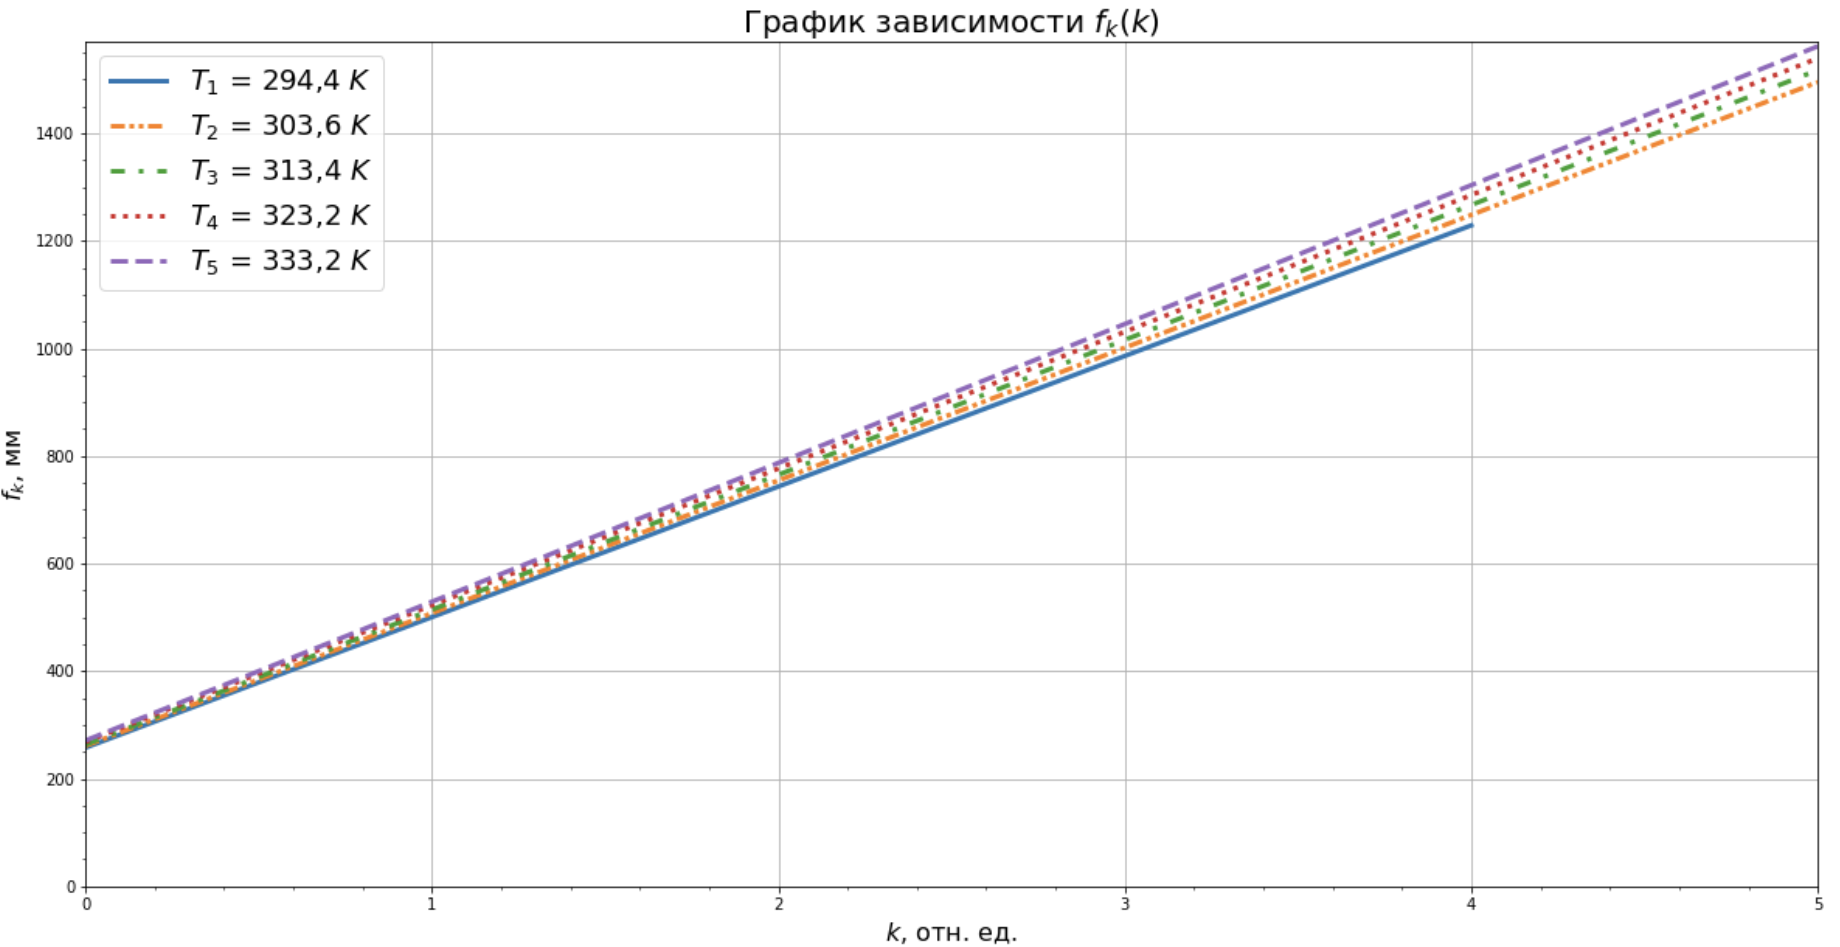
\includegraphics[scale=0.542]{graph2}
		\caption{Зависимость $ f_k $ от $ k $}
		\label{graph}
	\end{figure}

	Аппроксимируем полученные зависимости прямыми $ y=ax $ используя метод наименьших квадратов. Коэффициент $ a $ и погрешности его определения находим согласно формулам \eqref{mnk:a}, \eqref{mnk:sigma_a} и \eqref{mnk:full_sigma}. Результаты вычислений для каждой температуры заносим в таблицу \ref{tab:resConstL}.
	
	\begin{table}[H]
		\centering
		\begin{tabular}{|c|c|c|c|c|c|c|}
			\hline
			$ T $, К & $ a $, с$ ^{-1} $ & $ \sigma_a $, с$ ^{-1} $ & $ c $, м/с & $ \sigma_c $, м/с & $ \gamma $ & $ \sigma_\gamma $ \\ \hline
			294,4 & 242,8 & 1,3 & 339,9 & 1,8 & 1,369 & 0,007 \\ \hline
			303,6 & 246,9 & 0,9 & 345,7 & 1,3 & 1,373 & 0,005 \\ \hline
			313,4 & 250,8 & 1,0 & 351,1 & 1,4 & 1,372 & 0,005 \\ \hline
			323,2 & 254,3 & 0,9 & 356,0 & 1,3 & 1,368 & 0,005 \\ \hline
			333,2 & 258,2 & 0,8 & 361,5 & 01,2 & 1,368 & 0,005 \\ \hline
		\end{tabular}
		\caption{Результаты вычислений при различных температурах}
		\label{tab:resConstL}
	\end{table}
	
	Также, согласно формуле \eqref{5}, коэффициент наклона $ \displaystyle a = \frac{c}{2L}$. Тогда вычислим скорость звука $ c $ при фиксированной температуре и её погрешность, результаты вычислений занесём в таблицу \ref{tab:resConstL}.
	
	Кроме того, по формуле \eqref{gamma} вычислим $ \gamma $ при фиксированной температуре и погрешность этого вычисления. Результаты занесём в таблицу $ \ref{tab:resConstL} $. 
	
	Согласно полученным данным, можно утверждать, что $ \gamma $ остаётся постоянной в исследуемом диапазоне температур. Поэтому усредним результаты, полученные при различных значениях температуры и получим для воздуха:
	
	\[ \gamma = 1,37 \pm 0,01 \ (\varepsilon=0,4\%) \]
	
	\section{Выводы}
	
	В ходе выполнения работы мы:
	
	\begin{itemize}
		\item измерили частоту колебаний и длину волны при резонансе звуковых колебаний в газе, заполняющем экспериментальную установку;
		\item определили разными методами показатель адиабаты с помощью уравнения состояния идеального газа.
	\end{itemize}
	
	В ходе работы показатель адиабаты для воздуха был измерен двумя разными способами. Сначала измерения проводились при фиксированной частоте звукового сигнала, а мы изменяли длину трубы. В ходе таких измерения было получено:
	
	\[ \gamma_f = 1,41 \pm 0,01 \ (\varepsilon=0,6\%) \]
	
	Затем измерения проводились на другой установке, на которой длина трубы оставалась постоянной на протяжении всего опыта, а резонанса мы добивались при помощи изменения частоты звукового сигнала. В ходе этих измерений также исследовалась зависимость коэффициента адиабаты $ \gamma $ от температуры газа. Было получено, что показатель адиабаты не зависит от температуры в диапазоне температур $ 20-60 $ $ ^\circ C $ и равняется:
	
	\[ \gamma_L = 1,37 \pm 0,01 \ (\varepsilon=0,6\%) \]
	
	Сравним полученные данные с табличными. Согласно справочнику, показатель адиабаты для воздуха при нормальных условиях равен $ \gamma = 1,4 $. Таким образом, можно утверждать, что результат измерения $ \gamma $ на первой установке в пределах погрешности совпадает с табличными данными. Результаты измерения на второй установке незначительно отличаются от табличных. Это может быть связано с большой неточностью определения резонансных частот на второй установке. Чтобы этого избежать, необходимо использовать генератор частоты с возможностью более точной настройки для возможности четкого отслеживания резонансов.
	
	Также в ходе работы был измерен показатель адиабаты для углекислого газа. Измерения проводились на первой установке. В итоге мы получили \[ {\gamma_{CO_2} = 1,27 \pm 0,02}\ (\varepsilon=1,4\%) \]
	
	Сравним эти данные с табличными. Согласно справочнику, показатель адиабаты для углекислого газа при нормальных условиях $ \gamma = 1,3 $. Таким образом, полученные данные незначительно отличаются от табличных. Это может быть связано с тем, что при измерениях в трубе находился углекислый газ с примесями (в основном, азот и кислород), которые могли исказить результаты измерений. Для повышения точности, эксперимент стоит проводить в атмосфере углекислого газа, чтобы исключить попадание различных примесей в трубу.
	
	
	
	
	
	
\end{document}
